\makesavenoteenv{tabular}
\makesavenoteenv{table}


\lstset{%
basicstyle=\ttfamily\small,
breaklines = true,
tabsize=1
}
% \makeatletter
% \patchcmd{\maketitle}
% 	{\@maketitle}
% 	{\vspace{0em}\@maketitle\vspace{0em}}% change the value as needed
% 	{}
% 	{}
% \makeatother


% Watermarking
% \usepackage{draftwatermark}
% \SetWatermarkText{Draft: do not distribute}
% \SetWatermarkScale{0.4}
\setminted[python]{breaklines, fontsize=\footnotesize}
%\renewcommand{\listingscaption}{Policy}



\def\name{ESCHER}
\def\resadjective{Ephemeral}
\def\ray{Ray}
\def\createresapi{\textit{create\_resource}}

\newif\ifcomments
%%%KILL SWITCH for comments
%\commentstrue
\commentsfalse
\ifcomments
\newcommand{\rliaw}[1]{\textbf{\textcolor{red}{Richard: #1}}}
\newcommand{\alexey}[1]{\textbf{\textcolor{purple}{AT: #1}}}
\newcommand{\romil}[1]{\textbf{\textcolor{orange}{Romil: #1}}}
\newcommand{\romilc}[1]{\textbf{\textcolor{orange}{#1}}}
\newcommand{\swang}[1]{\textbf{\textcolor{blue}{Stephanie: #1}}}
% \newcommand{\ion}[1]{\textcolor{green}{Ion: #1}}
\newcommand{\camready}[1]{{\textcolor{blue}{#1}}}
%\newcommand{\suggest}[1]{\textcolor{violet}{#1}}Question 1 (Security):

\else
\newcommand{\rliaw}[1]{\textcolor{black}{}}
\newcommand{\alexey}[1]{\textcolor{black}{}}
% \newcommand{\romil}[1]{\textcolor{black}{}}
\newcommand{\swang}[1]{\textcolor{black}{}}
% \newcommand{\ion}[1]{\textcolor{black}{}}
\newcommand{\suggest}[1]{\textcolor{black}{}}
\newcommand{\nsdi}[1]{\textcolor{black}{}}
\newcommand{\camready}[1]{{{#1}}}
\fi


%\title[\name{}: Expressive Scheduling with \resadjective{} Resources]{\huge{\name{}: Expressive Scheduling with \resadjective{} Resources}}

\chapter[\name{}]{{\name{}: Expressive Scheduling with \resadjective{} Resources}} % Use short name ESCHER for headers
\label{ch_escher}

% Disable hyperlinks if you get errors in compilation
% \hypersetup{draft}

In this chapter, we take a close look at the top layer of the stack - the orchestration layer. As distributed applications become increasingly complex, maintaining high resource efficiency requires strict scheduling requirements. This development calls for cluster schedulers that are not only general, but also evolvable. Unfortunately, most existing cluster schedulers are not evolvable: when confronted with new requirements, they need major rewrites to support these requirements. Examples include gang-scheduling support in Kubernetes~\cite{spark-ganscheduling, kubernetes} or task-affinity in Spark~\cite{spark-ganscheduling}. Some cluster schedulers~\cite{omega,mesos} expose physical resources to applications to address this. While these approaches are evolvable, they push the burden of implementing scheduling mechanisms in addition to the policies entirely to the application.

\name{} is a cluster scheduler design that achieves both evolvability and application-level simplicity. \name{} uses an abstraction exposed by several recent frameworks (which we call \textit{ephemeral resources}) that lets the application express scheduling constraints as resource requirements. These requirements are then satisfied by a simple mechanism matching resource demands to available resources. We implement \name{} on Kubernetes and Ray, and show that this abstraction can be used to express common policies offered by monolithic schedulers while allowing applications to easily create new custom policies hitherto unsupported.

% \renewcommand{\shortauthors}{R. Bhardwaj et al.}

\section{Introduction}
\label{sec:intro}

With the end of Moore’s law and Dennard scaling, developers are forced to distribute their applications to process an ever growing amount of data. As a result, the past decade has seen a proliferation of new distributed frameworks~\cite{kubernetes, ray-osdi, mesos} to handle a variety of workloads from big data (e.g., batch jobs, interactive query processing) to AI applications (e.g., model training and serving).


% https://docs.google.com/drawings/d/1jXbZJhnhrtNHtrjuyGhHoiT4LbjzwVerwn02Tnw-Kv0/edit
\begin{figure*}[ht]
\centering
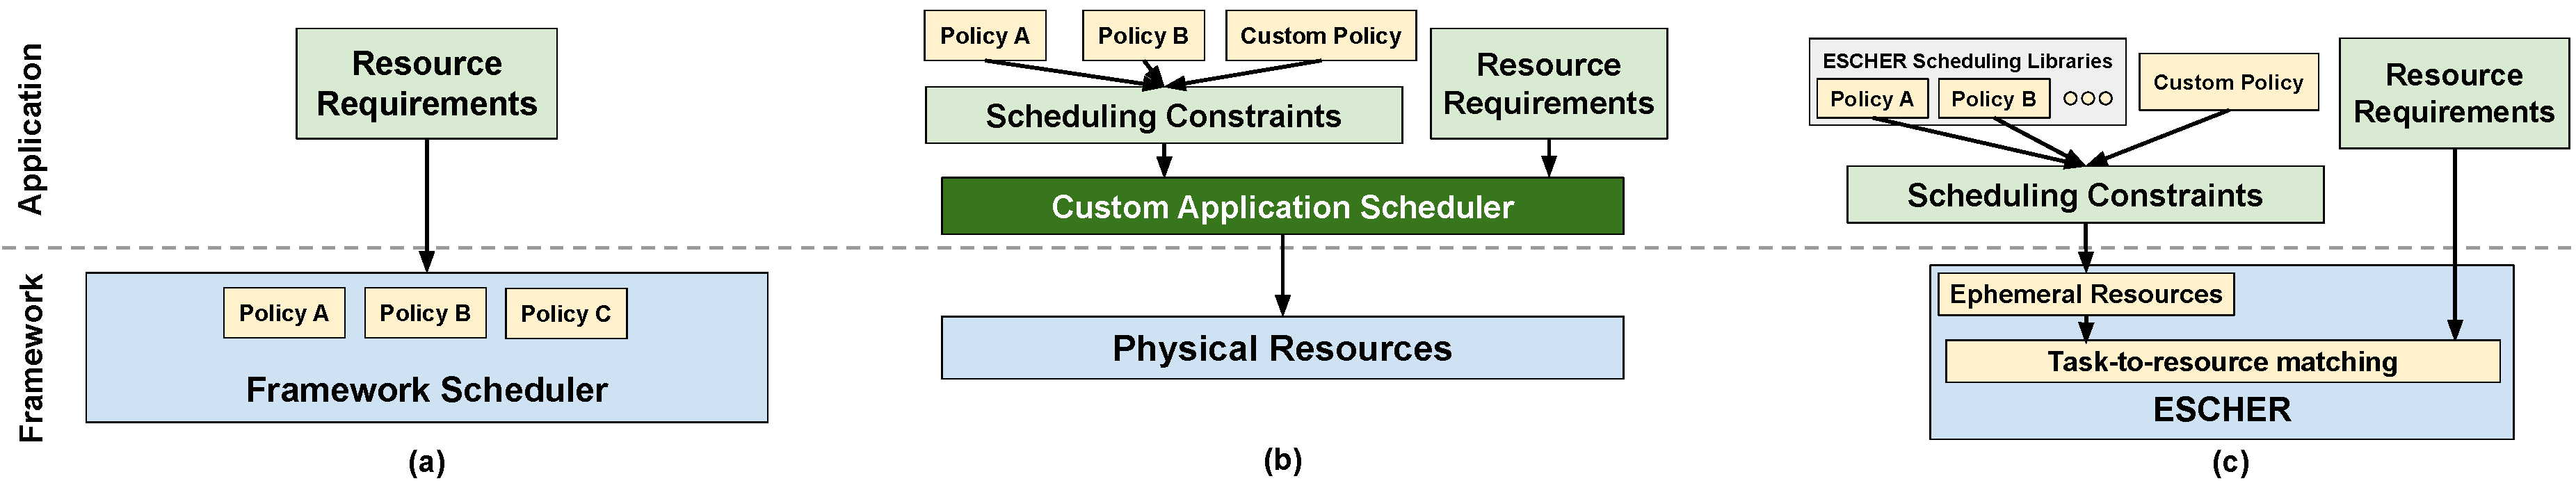
\includegraphics[width=0.92\linewidth]{escher/figures/escher-compare-arch.pdf}
\caption{\small
\textbf{(a)} A monolithic scheduler implements both scheduling and resource constraint matching~\cite{ghodsi2011dominant,isardquincy,mpi,kubernetes}. Some schedulers allow applications to express and compose certain policies~\cite{condor,tetrisched,kubernetes}, but custom application policies may require modifying the scheduler itself.
% Though this API abstracts away scheduling logic from the application, it is not expressive enough to allow applications to express compositions of scheduling policies.
\textbf{(b)} To maximize flexibility, some frameworks expose physical resources \cite{mesos, omega}, but require applications to write custom schedulers that manage both policy and resource coordination~\cite{gandiva,DevinMasters,mapreduce}.
%This burdens the application developer with explicitly handling resource allocation.
\textbf{(c)} \name{}. With ephemeral resources, applications can express custom policies through ephemeral resources, while the cluster scheduler provides just one service - satisfying per-task resource constraints.
}
\label{fig:scheduler-architectures-new}
\vspace{-2mm}
\end{figure*}

% Introduce evolving policy requirements
As the number of data and AI applications grows, so do their scheduling requirements. 
%Different applications demand different scheduling policies from these frameworks. 
Some examples of scheduling policies are \emph{affinity} (i.e., co-locate computation with data to avoid costly data transfers), \emph{anti-affinity}  (i.e., schedule tasks on different machines to avoid interference), 
%\emph{load balancing} (e.g., distribute requests round-robin across multiple servers), 
and \emph{gang scheduling} (i.e., schedule a group of interdependent tasks simultaneously). For example, a hyperparameter search application~\cite{hypersched,gandiva} consists of multiple distributed training jobs, each consisting of multiple parallel tasks. This requires anti-affinity between jobs for high throughput, affinity within a job to avoid unnecessary data transfers, and gang scheduling to ensure multi-node jobs are not starved. 
%Worse yet, some of these application policy demands emerge after the scheduling framework has been released.

% Current scheduling landscape
This diversity of policy requirements makes designing schedulers for distributed frameworks challenging. There is an inherent trade-off between \emph{simplicity} and \emph{flexibility} in exposing different policies to applications. Different cluster managers occupy different points in this trade-off space. 

At one end of the spectrum (Figure \ref{fig:scheduler-architectures-new}a), monolithic cluster managers like YARN~\cite{yarn} and Kubernetes~\cite{kubernetes} provide several out-of-the-box policies for the application to chose from. This simplifies the application's task, but it compromises the flexibility, as adding a new policy requires changes to the scheduler and the cluster manager itself. Implementing a new policy requires the developer to understand and modify the source code of the cluster manager, not always an easy task given their inherent complexity. And, once the new policy is implemented, the developer is on the horns of a dilemma: either fork the project and pay the cost of maintaining it up-to-date as the project evolves, or wait many months for the change to be merged in the main branch. Worse yet, if the cluster manager is closed source, the application developer has no choice but to wait and hope that the company behind the cluster manager will implement the desired policy.

At the other end of the spectrum (Figure \ref{fig:scheduler-architectures-new}b), are schedulers like Omega~\cite{omega} and Mesos~\cite{mesos} that enable an application to directly allocate resources and implement its own scheduling logic. This makes these cluster managers very flexible, but dramatically increases the complexity of the application. Implementing a scheduling policy in a distributed system can be a daunting task, as it requires not only allocating resources, but tracking the resource availability in the presence of various failures and new nodes joining the system.

%Moreover, keeping the fork of the source code up-to date with the upstream master branch can be tedious and requires constant maintenance.
% Explain why this landscape is not sufficient
%The cluster managers in the first category simplify the applications by implementing the entire scheduling logic, but compromise the flexibility, as adding a new policy requires changes to the scheduler and to the cluster manager itself. 

%Implementing a new policy requires the application developer to understand and modify the source code of the cluster manager. This requires in-depth knowledge of the cluster manager which the developer might not be familiar with. Moreover, keeping the fork of the source code up-to date with the upstream master branch can be tedious and requires constant maintenance. Cluster managers in the second category are highly evolvable, as the applications can implement any scheduling policy they want. This comes at the cost of complexity, as implementing a scheduler in a distributed system requires not just allocating resources to tasks, but also tracking resource availability in a distributed, fault-prone environment.


% Introduce virtual resources
In this work, we present another point in the design space that allows application developers to easily implement a range of new scheduling policies. This design point is enabled by a mechanism recently introduced by cluster managers like Kubernetes and Ray which provides an interface for applications to dynamically create, modify, and destroy logical resources. We call these resources \emph{ephemeral resources}.  Like regular resources, ephemeral resources are pairs of labels and count values which can be allocated to tasks. The scheduler treats ephemeral resources in the same way as physical resources, subjecting them to admission control to ensure they are not oversubscribed. This frees the applications from performing admission control and tracking availability.

%Interestingly, in addition to these mechanisms, some cluster schedulers provide an interface for users to dynamically create and modify \emph{virtual} resources on physical nodes in the cluster. Like regular resources, \emph{virtual} resources are pairs of labels and count values which can be allocated to tasks. For instance, in Kubernetes and Ray, users can create resources on nodes to identify specialized accelerators (e.g. {Nvidia V100 GPU: 4}). These virtual resources can then be requested by tasks, and the cluster scheduler ensures that tasks are placed on nodes where resources are available. The cluster scheduler treats virtual resources the same as physical resources, subjecting them to admission control to ensure they are not oversubscribed. 

% Give example of scheduling with ephemeral resources
We find that a surprisingly large number of scheduling policies can be expressed by dynamically creating, updating and destroying ephemeral resources. Consider a simple scheduling constraint to colocate two tasks T1 and T2. To express this constraint, an application would submit T1, which creates an ephemeral resource R1 during execution, and then submit T2 with R1 as a resource requirement. The scheduler is then forced to place T2 on the same node as T1, since no other node has resource R1. While this is a very simple example, it illustrates the underutilized power of ephemeral resources for satisfying application-level scheduling constraints. In contrast, a monolithic cluster manager would have to expose a primitive designed specifically for task-task affinity, and a two-level scheduler application would have to implement the entire policy themselves, choosing where \emph{both} T1 and T2 execute.

% Raise the thesis of this paper
%This raises a natural question - by dynamically creating ephemeral resources and requesting them in task resource requirements, can applications express and satisfy their scheduling constraints? In this paper evaluate this question through the lens of generality (can ephemeral resources satisfy a wide range of scheduling constraints?), performance (is scheduling with ephemeral resources as performant as modifying the core scheduler?) and simplicity (how easy is it for applications to use ephemeral resources?).

%\ion{This is the key paragraph that must state super clearly why emphemeral resources are useful and what are the questions we want to answer in this paper.} 
The key promise of ephemeral resources is that they enable an application to implement new scheduling policies \emph{not} supported by the underlying cluster manager. This increases the velocity of deploying and iterating on new application functionality. % and thus reduces the time to value for new products and features.
However, there are two natural questions that follow. First, how general are the scheduling policies enabled by ephemeral resources? Second, what are the costs in terms of implementation complexity and overhead compared to natively implementing the same policy in the cluster manager?
After all, if these overheads dominate, then an application developer is better off building their own scheduler.

To answer these questions, we propose a scheduling architecture for distributed applications called ESCHER \footnote{\name{} stands for Expressive SCHeduling with Ephemeral Resources.}.
In ESCHER, the application uses ephemeral resources to implement its scheduling policy instead of relying on the cluster manager's baked-in policies.
The key insight of ESCHER is that a broad class of heterogeneous scheduling constraints can be cast as \emph{ephemeral resource requirements}. The underlying scheduler simply enforces these requirements. ESCHER enables applications to implement a large number of scheduling policies by (1) dynamically creating new ephemeral resources, and (2) specifying task resource requirements on these ephemeral resources. We find that by using these two simple primitives, we are able to satisfy a large set of scheduling constraints, without requiring any changes to the core scheduler or significantly affecting application performance. For instance, gang-scheduling in ESCHER can be written in 10x fewer lines of code with less than 2x overhead in scheduling latency compared to implementing the policy natively in the core scheduler (\cref{sec:eval:gangscheduling}).

%\romilc{The reason \name{} simplifies implementing new policies at the application level is because the core scheduler fulfills a singular responsibility - satisfying a task's resource demands (ephemeral and physical).
%This responsibility implies that only resource tracking and coordination (resource acquisition and release) be implemented by the core scheduler.
%The application satisfies its scheduling constraints by specifying per-task ephemeral resource requirements and manipulating these ephemeral resources over the lifespan of the application.}
%Effectively, \name{} enables a broad class of \textit{heterogeneous scheduling constraints to be cast as ephemeral resource requirements}. 

% Tradeoffs with ephemeral resources.
However, the flexibility of ephemeral resources does not come for free. First, it increases the application complexity compared to monolithic schedulers in which applications just need to select one of the available policies. Implementing certain policies, such as gang scheduling, requires the application to implement additional mechanisms using ephemeral resources such as ghost tasks, i.e., tasks whose sole purpose is to signal when all required resources have been allocated. Second, because ephemeral resources are created dynamically, an application must handle infeasible requests explicitly. For example, if a task's resource request cannot be satisfied, the task will hang and it must be explicitly terminated.% the application must explicitly terminate it. 
%Second, ephemeral resources need to be \emph{handled with care}. In cases when an application makes a request of ephemeral resources that is not feasible, the application might have to roll back and free the ephemeral resources it has allocated.  This is akin to the way memory management (malloc, free) is handled in many low-level programming languages. 
% Finally, debugging is challenging as it requires logging and replaying the ephemeral resource creations and deletions.
%Finally, since ephemeral resources are declarative in nature, debugging them requires replay of resource creation/deletion logs, which can be challenging.

% Second, because the ESCHER architecture provides no visibility into the global cluster state, tasks in multi-tenant environments have slightly reduced performance due to the back-off based collision avoidance in ESCHER.

% Tradeoff mitigation
%which reduce implementation burden of applications for common policies.
To alleviate the challenge of application complexity and provide protection against invalid resource specifications, ESCHER supports  simple libraries to support common policies. We call these libraries \name{} Scheduling Libraries (ESLs). ESLs aim to provide the best of both worlds: the simplicity of monolithic schedulers, and the flexibility of adding new scheduling policies at the application level by either extending an existing ESL or creating a new one. ESLs decouple application logic and policy by abstracting ephemeral resource management for common high-level scheduling policies, thus dramatically reducing development cost via code reuse and enabling composition of simple policies into more complex ones. % ESLs compose with other ESLs as well as custom policies. %Thus, ESLs offer the benefits of modularity, such as policy composition and reuse, while still allowing applications to implement custom policies. 
%As the name suggests, ESLs are akin to libraries in today's programming languages which implement the most common functionality and expose it to developers through simple APIs, thus dramatically reducing development cost via code reuse and enabling composition of simple policies into more complex ones.

%To evaluate \name{}, w
To evaluate \name{}'s performance, we implement it on both Kubernetes~\cite{kubernetes} and Ray~\cite{ray-osdi} by leveraging their existing implementations 
%\swang{was it existing for Ray? I thought that we implemented it for this paper}
% of ephemeral resources.
for label-based scheduling, which were originally intended to represent custom physical resources rather than logical scheduling constraints.
We run \name{} on a range of applications and policies, including  WordCount MapReduce with max-min fair sharing on Kubernetes as well as
AlphaZero~\cite{silver2016alphago} and distributed model training on Ray~\cite{ray-osdi}. We show that \name{} does not impact the end-to-end performance of most applications when compared to a system that implements the same policies in the core scheduler. Meanwhile, the application can use \name{} to express additional policies not supported by the underlying core scheduler, e.g., composing gang scheduling with affinity~(\Cref{sec:eval:tune}). %increase the completion times of some applications, e.g., applications consisting of sub-millisecond level tasks. 
%\ion{I find the point that we can use ESCHER to implement the policy in the core scheduler confusing. I'd just say that in some cases there is overhead and give one or two examples of such cases.}
%\romilc{While the performance of \name{} is largely comparable to policies hard-coded in a monolithic scheduler, the application-level mechanisms used to implement policies can add to the scheduling latency for some workloads. However, if performance is a priority, ESCHER can also be used to implement policies at the system level by modifying the core scheduler. In \Cref{sec:eval}, we evaluate the tradeoffs involved in moving policies to the system level.}
%In the process, we show that \name{}~is able to match the performance of comparable policies hard-coded in a monolithic scheduler.

Thus, \name{} shows that one can take advantage of the ephemeral resource abstraction, whose implementation is already partially provided by some cluster managers, to express a surprisingly diverse set of scheduling policies at the application level without having to touch the core scheduler. This allows users to quickly implement new policies, as needed, to improve support for their applications.

% To reiterate, the main point of this paper is not to claim that implementing a scheduling policy using ephemeral resources is better than implementing it in the cluster's core scheduler, or that it is the best mechanism to implement an extensible scheduling architecture. Rather, our goal is to show that one can take advantage of the ephemeral resource abstraction already provided by existing cluster managers to implement a surprisingly diverse set of scheduling policies at the application level, without having to touch the core scheduler. This allows users to quickly implement new policies, as needed, to improve support for their applications.

%Effectively, \name{} trades a small loss in performance in favor of significant increase in the flexibility of the scheduler to support new policies.
In summary, we make the following contributions: 

\begin{compactitem}
    \item \name{}, a scheduling architecture that uses ephemeral resources to express scheduling policies without modification to the core scheduler.
    % \item An evolvable scheduler design that uses a simple resource-matching scheduler, allowing applications to express policies with ephemeral resources.
    % \item We show that ephemeral resources can support existing policies with little performance degradation completely in the application space.
    \item Design and implementation of a wide class of scheduling policies (\S\ref{policies}) using the ephemeral resources API.
    % \item Support for new policies through \emph{dynamic} creation and destruction of ephemeral resources.
    % \item We show that it is possible to implement a general scheduler and to express policies in the application space, including dynamic and composed policies, with one simple abstraction, ephemeral resources, and one simple mechanism, task-to-resource matching.
    \item ESLs: application-level scheduling libraries that enable applications to easily compose and re-use policies.
    % \item We show that policies implemented by the applications with ESCHER can match the performance of equivalent policies implemented natively by the framework. % The resource management is still handled by the framework 
\end{compactitem}





% 1. Put the sentence at the start of the - despite these tradeoff, ephemeral resources are the only method that provides the user ability to implement besides modifying the core scheduler for dominant monolithic schedulers. .

% 2. "We find that a surpsingly" comes too late. Maybe add that before you introduce the mechanism. Another point in the design space. 

% Ephemeral resources. 
% Virtual -> Logical
% Epheemeral resources are dynamic short-term resources. Can be programatically created and destroyed.

% Debugging is challenging because you don't know when resources are created and deleted. 

% ESLs - If I have a ESL, why not in core scheduler?

\section{Motivation}
\label{sec:escher_motivation}


% \begin{table*}[]
% \begin{tabular}{|l|l|l|}
% \hline
%                                          & \textbf{ESCHER}                          & \textbf{Omega}                                   \\ \hline
% \textbf{Scheduler implementation by}     & Framework (constraints specified by application) & Application                                      \\ \hline
% \textbf{Best suited for}                      & Short lived tasks                        & Long running tasks (fewer OCC conflicts)          \\ \hline
% \textbf{Concurrency model}               & Resource ownership granted by parent ESL & Optimistic concurrency control with shared state \\ \hline
% \textbf{Cluster-wide policy enforcement} & Managed by parent ESL                    & Free-for-all, hard to enforce cluster policies   \\ \hline
% \textbf{Conflict resolution} & Done by framework                    & Done by application   \\ \hline
% \end{tabular}
% \caption{ESCHER vs Omega}

% \end{table*}

%\name{} is motivated by the need of many modern distributed applications for fine-grained scheduling control.
\Cref{tab:sched-pols} lists some common scheduling policies required by modern distributed applications and their off-the-shelf support across different frameworks and specialized schedulers. 
None of the schedulers support all policies, and many were built as a one-off solution to achieve a composition of these policies. 
New applications which require a new policy must find alternate methods of executing it - either by using some mechanism provided by the scheduler, such as labels, or writing their own scheduler from scratch. %\romil{Move the labels to after distributed training?}
We now give a motivating example that is insufficiently served by existing schedulers and describe how \name{} fills this gap.
%As a result, researchers and practitioners have developed specialized frameworks to support these workloads. Unfortunately, building such one-off solutions is expensive and does not scale. 

% https://docs.google.com/spreadsheets/d/16M7Ia2e4X7hofFKPAhwRx6LiYlhBFzlqwzldHgewwCQ/edit?usp=sharing
%\newcommand{\centered}[1]{\begin{tabular}{l} #1 \end{tabular}}
\newcommand\colw{0.8}

\newcommand{\xmark}{\ding{55}}

\begin{table}[!t]
  \small
  \centering
  \begin{xtabular}{|p{0.45\linewidth}|
  p{\colw em}|p{1.6em}|p{\colw em}||p{\colw em}|p{\colw em}|p{\colw em}|}
  \cline{2-7}
  \multicolumn{1}{c|}{}  &  \multicolumn{3}{c||}{\textbf{Framework}} & \multicolumn{3}{c|}{\textbf{Scheduler}}\\
  \hline
    \textbf{Policy} 
  \vspace{13mm} & 
  \textbf{\rotatebox[origin=c]{90}{YARN CS~\cite{yarn}}} &
  \textbf{\rotatebox[origin=c]{90}{\parbox{2.2cm}{Kubernetes~\cite{kubernetes} Core / Labels}}} &
  \textbf{\rotatebox[origin=c]{90}{Spark~\cite{spark}}} &
  \textbf{\rotatebox[origin=c]{90}{Sparrow~\cite{sparrow}}} &
  \textbf{\rotatebox[origin=c]{90}{Gandiva~\cite{gandiva}}} &
  \textbf{\rotatebox[origin=c]{90}{Gorila~\cite{gorila}}}
  \\
  \hline
  
  % Begin info
  
  \textbf{Task co-location}\newline
  Place $n$ tasks on the same physical machine.
  %\vspace{1mm}
    % \begin{minted}[autogobble]{python}
    % coloc_tasks = [...]
    % res_constraint = sum([t.resources for t in coloc_tasks])
    % set_resource("coloc-group", len(coloc_tasks), res_constraint)
    % for task in coloc_tasks:
    %     task.launch(resources={"coloc-group": 1})
    % \end{minted}
  &
  $\checkmark$& % YARN CS
  $\checkmark\text{/\checkmark}$& % Kubernetes
  $\text{\xmark}$& % Spark
  $\checkmark$& % Sparrow
  $\checkmark$& % Gandiva
  $\checkmark$% Gorila
  \\
  \hline
  
  \textbf{Data locality}\newline
  Place tasks with operands.
  \vspace{0.01em}
    % \begin{minted}[autogobble]{python}
    % data_addr = nodeid  # Node id where the data is
    % set_resource("data-loc", 1, data_addr)
    % task.launch(resources={"data-loc": 1})
    % \end{minted}
  &
  $\checkmark$& % YARN CS
  $\checkmark\text{/\checkmark}$& % Kubernetes
  $\checkmark$& % Spark
  $\checkmark$& % Sparrow
  $\text{\xmark}$& % Gandiva
  $\text{\xmark}$ % Gorila
  \\
  \hline
  
%   \textbf{Static Load Balancing}\newline
%   Given $n$ tasks, evenly spread them out across $m$ workers.
%   %\vspace{1mm} 
% %     \begin{minted}[autogobble]{python}
% %   resource_capacity = ceiling(num_tasks/num_nodes)
% %   for node in nodes:
% %     set_resource("load_bal", resource_capacity, node)
% %   for task in tasks:
% %     task.launch(resources = {"load_bal": 1})
% %     \end{minted}
%   &
%   $\checkmark$& % YARN CS
%   $\checkmark\text{/\checkmark}$& % Kubernetes
%   $\checkmark$& % Spark
%   $\checkmark$& % Sparrow
%   $\checkmark$& % Gandiva
%   $\checkmark$% Gorila
%   \\
%   \hline
  
  \textbf{Elastic Load Balancing}\newline
  Given an unknown number of tasks, evenly spread them out across $m$ workers. 
  \vspace{-4mm}
%   \begin{minted}[autogobble]{python}
%     def load_monitor():
%       while True:
%         avail_res = get_cluster_status()
%         if avail_res["load_bal"] == 0 on all nodes:
%             set_resource("load_bal", increment 1, all_nodes)
%         if avail_res["load_bal"] >= 1 on all nodes:
%             set_resource("load_bal", decrement 1, all_nodes)

%     def dynamic_load_balancing():
%       load_monitor.launch()
%       for task in tasks:
%         task.resources = {"load_bal": 1}
%         task.launch()
%     \end{minted}
  &
  $\checkmark$& % YARN CS
  $\checkmark$\text{{/\xmark}}& % Kubernetes
  $\text{\xmark}$& % Spark
  $\checkmark$& % Sparrow
  $\checkmark$& % Gandiva
  $\checkmark$% Gorila
  \\
  \hline
  
  \textbf{Bin-packing}\newline 
  Given an unknown number of incoming tasks, minimize the number of workers used to complete the tasks.
  %\vspace{1mm}
  &
  $\checkmark$& % YARN CS
  $\checkmark$\text{{/\xmark}}& % Kubernetes
  $\text{\xmark}$& % Spark
  $\text{\xmark}$& % Sparrow
  $\checkmark$& % Gandiva
  $\text{\xmark}$% Gorila
  \\
  \hline
  
  \textbf{Anti-affinity}\newline 
  Given two tasks, place them on distinct nodes.
  &
  $\checkmark$& % YARN CS
  $\checkmark$\text{{/\checkmark}}& % Kubernetes
  $\text{\xmark}$& % Spark
  $\text{\xmark}$& % Sparrow
  $\checkmark$& % Gandiva
  $\text{\xmark}$% Gorila
  \\
  \hline
  
  \textbf{Gang scheduling}\newline 
  Given a set of tasks, enforce all-or-none run semantics.
  \vspace{1mm}
  &
  $\text{\xmark}$& % YARN CS
  $\text{\xmark}\text{{/\xmark}}$& % Kubernetes
  $\checkmark$& % Spark
  $\text{\xmark}$& % Sparrow
  $\text{\xmark}$& % Gandiva
  $\checkmark$% Gorila
  \\
  \hline
  
  \textbf{Weighted Fair Queuing\cite{wfq}}\newline 
  Given a set of tasks, enforce priority ordering. 
  &
  $\checkmark$& % YARN CS
  $\checkmark\text{{/\xmark}}$& % Kubernetes
  $\checkmark$& % Spark
  $\checkmark$& % Sparrow
  $\text{\xmark}$& % Gandiva
  $\text{\xmark}$% Gorila
  \\
  \hline

  \textbf{Soft-constraints}\newline  
  For a priority ordering of resource constraints, schedule a task with the highest possible resource satisfiability.
  &
  $\text{\xmark}$& % YARN CS
  $\checkmark\text{{/\xmark}}$& % Kubernetes
  $\text{\xmark}$& % Spark
  $\text{\xmark}$& % Sparrow
  $\text{\xmark}$& % Gandiva
  $\text{\xmark}$% Gorila
  \\
  \hline
  
  \end{xtabular}
  \vspace{2mm}
  \caption{\small Common scheduling policies and off-the-shelf support from existing schedulers. Kubernetes comparision includes both modes of operation, using just the core scheduling functionality and using labels. In addition to these policies, ephemeral resources allow applications to specify and compose custom policies.
  %\romil{Once format is approved, reorder columns to fit the category. Frameworks: YARN, Kubernetes, Spark}
  %\swang{Make the vertical line between "Frameworks" and "Schedulers" bold}
  }
  \label{tab:sched-pols}
\end{table}

\subsection{Existing systems are hard to evolve}
\label{sec:escher_motivation:example}

% As model size increases, 
As applications become increasingly diverse, cluster schedulers must evolve to support novel scheduling policies required by these applications. Consider distributed training, a dominant ML workload today. 
Multiple training jobs are often scheduled simultaneously due to multi-tenancy and individual users submitting multiple training runs in parallel to evaluate different model architectures.
This requires several distinct scheduling policies: % \rliaw{we can say something stronger here right? it's not simply an issue of supporting, there's also a hierarchical relationship}
\begin{compactitem}
\item \emph{Anti-affinity:} Evenly spread training jobs across the cluster to ensure high throughput.
\item \emph{Affinity:} Co-locate all tasks of the same training job on the same machine to avoid unnecessary data transfers.
\item \emph{Gang scheduling:} For multi-node jobs, schedule all tasks of the job simultaneously to avoid starvation.
\item \emph{Bin packing (dynamic):} Monitor job utilization and consolidate jobs to reduce resource fragmentation. % TODO: And reduce network transfers.
\end{compactitem}

Many popular schedulers implement at least one of these policies, but it is rare for them to support all four~(\Cref{tab:sched-pols}), never mind a composition of the policies.
% Monolithic schedulers tightly couple the scheduling policy and mechanism~(\Cref{fig:scheduler-architectures}a).
There are two fundamental challenges that make it difficult or infeasible to extend monolithic schedulers~(\Cref{fig:scheduler-architectures-new}a) in this way.
We use Kubernetes~\cite{kubernetes} to illustrate these challenges. %, but we stress that the following limitations are in fact \textit{fundamental} to monolithic schedulers.
% 

First, the application must \emph{express} its policy using the API chosen by the framework scheduler.
%Each scheduler exposes a different interface for policy specification.
While some schedulers support composition, it is difficult in general to design a scheduler API that can capture all possible use cases.
For example, in Kubernetes, applications specify scheduling policies with \emph{static weights} to resolve conflicts.
This can be used to express a composition of two policies that, for instance, weights affinity over anti-affinity.
However, the complexity of composition is not linear in the number of policies.
E.g., to add bin packing and prioritize it, the application would have to ensure that the weight of bin packing is always greater than the sum of weights for affinity and anti-affinity.
% Furthermore, dynamic policies like bin packing in this case cannot be expressed using only static weights.

Second, the scheduler \emph{implementation} must extend to new policies.
This is difficult because the scheduler must ensure that each new policy interfaces correctly with all other existing policies.
% This is difficult because of the tight coupling between scheduling policy and mechanism in monolithic schedulers.
% For example, while Kubernetes supports a range of policies, including affinity and anti-affinity, this list is not exhaustive.
Adding another policy requires modifying Kubernetes itself, which takes significant time and effort. Dynamic policies are even more difficult to support if the scheduler was not initially designed for it. For instance, adding gang scheduling support in Kubernetes took months of discussions and the eventual feature was not mainlined and instead implemented in an add-on scheduler ~\cite{kubernetes-gang-scheduling, kubernetes-gang-scheduling-first-comment, kubernetes-gang-scheduling-kubebatch-pr}.
Similarly, Machine Learning pipelines involve multiple interdependent tasks (e.g., data pre-processing, training, serving) defined in a DAG. Scheduling DAGs is not natively supported in Kubernetes, leading to the emergence of specialized plugins such as Kubeflow~\cite{kubeflow}.

% For example, the ability to correct previous scheduling decisions requires an entirely separate system to evict tasks in Kubernetes~\cite{kubernetes-descheduler}.
% Furthermore, this system only handles changes in the \emph{cluster} environment and does not allow changes in the \emph{application} policy.

Due to these limitations, applications must write custom schedulers to maximize performance, as Gandiva~\cite{gandiva} did for distributed training.
% Gandiva uses feedback from the application to dynamically adjust task placement, composing affinity, anti-affinity, and dynamic bin-packing.
Unfortunately, this design requires the application to implement both the policy and the scheduler \emph{mechanism}, maintaining resource state and handlers for task and resource management, coordination, node addition and deletion, etc.~(\Cref{fig:scheduler-architectures-new}b).
This is both difficult to build and extend.
E.g., Gandiva (built on Kubernetes) supports affinity, anti-affinity, and dynamic bin-packing, but the addition of gang scheduling would greatly increase the complexity of the scheduler code.
%\alexey{can we quantify this, Romil?}
Thus, Gandiva remains limited to distributed training jobs that fit on a single multi-GPU node.

% https://docs.google.com/drawings/d/1x6561xEY_K5CEV12J6dLwa7TMJqwGX-idUDL-PlSrb0/edit
% \begin{figure}[ht]
%     \centering
%     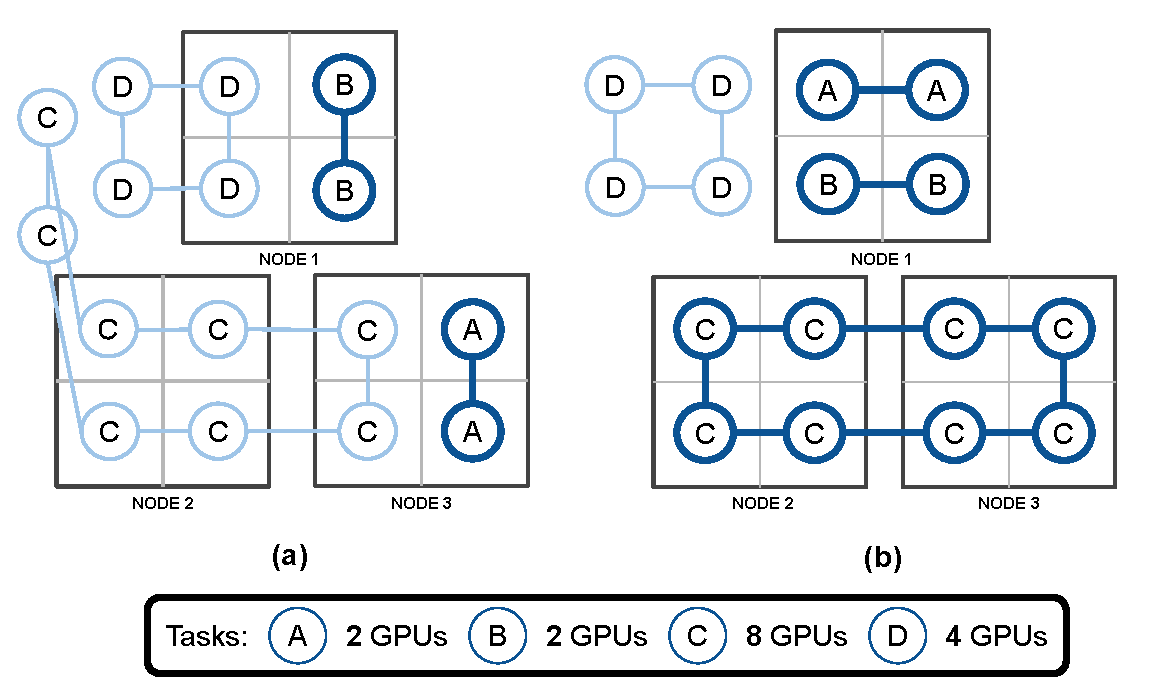
\includegraphics[width=0.95\linewidth]{escher/figures/ESCHER-training.pdf}
%     \caption{Task placement for 4 distributed training jobs on a cluster with 12 GPUs. Each training job comprises multiple tasks, and each task occupies 1 GPU. The jobs arrive in order from $A$-$D$, and all tasks can take a variable amount of time to start. Jobs can only make progress if all tasks are started (i.e., they require gang scheduling). \textbf{(a)} Task placement with affinity and anti-affinity, but no gang scheduling. $C$ has some tasks that are not placed before $D$ arrives, so neither $D$ nor $C$ can run. \textbf{(b)} Task placement with affinity, anti-affinity, and gang scheduling. $A$ is initially placed on Node 1 and $B$ on Node 2 (not shown). With gang scheduling, when $C$ arrives, $B$ can be migrated to Node 1 to allow $C$ to run. \romil{Candidate for cutting}}
%     \label{fig:distributed-training}
%     \vspace{-3mm}
% \end{figure}

\subsection{Static labels are insufficient}
\label{sec:escher_motivation:label}
Some frameworks~\cite{mesos,omega,yarn,kubernetes} already support \emph{static} label creation as string key-value pairs (e.g., "v100 GPU": 1) associated with cluster nodes.
This allows cluster operators to tag nodes with physical resource attributes (e.g., CPU/GPU architecture, rack affinity) at cluster launch time, which can be requested by applications at execution time.
%Then, at execution time, an application can request task placement on nodes with specific labels, using hard or soft constraints.

% Tasks can then request placement on nodes with specific labels.
% However, in today's cluster deployments, label creation is controlled by cluster operators, not applications. This enables applications to express constraints on desired properties (e.g., CPU/GPU architecture, rack affinity, availability zone). Soft constraints are also supported, but only relative to the resource attributes.

In \name{}, we propose repurposing this API to express \emph{custom application scheduling policies}, in addition to physical resource requirements.
Unlike physical resources, which can be statically determined at a node's launch time, logical scheduling constraints may depend on run-time information.
Therefore, it is natural to extend existing static label creation APIs to \emph{ephemeral resources} that are dynamically created.

For example, to express task-task affinity between tasks $T_1$ and $T_2$, we must first learn where $T_1$ was placed before deciding the placement constraint for $T_2$.
This can be easily done through ephemeral resources: $T_1$ dynamically creates a logical resource that is required by $T_2$.
With static labels, the only option is for the application to pin $T_1$ and $T_2$ to a predetermined node.

% To express \textit{inter-task }relationships, however, requires mapping them to existing statically created resource labels. E.g., task-task affinity can only be expressed by placing task $T_1$ first and then placing task $T_2$ second with a requirement for the node label where $T_1$ landed. With ability to \textit{dynamically} create labels, applications can express inter-task constraints in a single shot, without requiring for multiple scheduling round trips necessary in TetriSched~\cite{tetrisched} and Firmament~\cite{firmament}.

For the same reason, there are some inter-task constraints that are fundamentally impossible to implement with static labels, such as scheduling policies that depend on \emph{time}.
One example is a DAG scheduling policy.
At its core, this requires a primitive that guarantees that some task $T_2$ will not run until another task $T_1$ finishes.
This is impossible to express using static labels alone, which cannot reason about the temporal ordering between two tasks.

% with cyclical/iterative behavior~\cite{naiad-sosp13}. E.g., it is impossible to express the resource schedule for two tasks $T_1$ and $T_2$ that implement an iterative computational pattern (e.g., SGD gradient calculation and model update). Dynamic ephemeral resource creation in \name{} enables $T_i$ to create a label with a logical clock suffix, incremented to reflect the iteration epoch. Each task $T_i \in \{T_1,T_2\}$ then consumes a label from the previous iteration epoch, effectively unrolling the task graph cycle~\cite{naiad-sosp13}. Capturing such dynamic behavior requires a dynamic mechanism and cannot be expressed with state-of-the-art declarative frameworks~\cite{dcm-osdi20, tetrisched}.

% provide the ability to create labels, string key-value pairs (e.g. "partition: customerA") that can be associated with nodes. These labels can subsequently be specified as necessary qualifiers for a task to be scheduled (e.g. run task $T$ only where "partition" label is "customerA"). Granting applications the ability to create and remove labels can allow applications to express custom scheduling policies. For instance, co-location can be enforced by having two tasks request a unique label in their label requirements. However, exercising scheduling control with labels has two critical shortcomings which limits its generality.

% First, node labels are static. In today's deployments, the control of label creation and deletion is primarily owned by cluster operators, who create labels when a node is added to the cluster. This limits applications to using labels created by the operators. If applications are granted the ability to create node labels, they can implement a larger set of policies, such as data-locality by creating labels where the data is generated. 

% Second, labels do not have an associated numerical capacity. Unlike a resource, tasks cannot acquire or consume labels, which makes it difficult to express policies which rely on evaluating task counts or utilization on different nodes. For instance, performing load-balancing with key-value labels would require the application to create unique labels on each node and track the number of tasks requesting each label. This is equivalent to implementing the complete scheduling logic in the application space. % Kubernetes' extended resources \cite{kubernetesextres} improves on labels by adding a numerical capacity to labels, but it remains static in it's current usage.

% \subsection{An End-to-End Argument}
% \label{sec:escher_motivation:e2earg}

% \name{} applies the end-to-end principle~\cite{e2e-argument} to cluster scheduling by keeping the core scheduler mechanism simple yet scalable, while ephemeral resources provide applications with flexibility to express scheduling policies.
% Similar to Exokernel~\cite{exokernel}, \name{} focuses on enabling applications to implement custom scheduling policies in a heterogeneous distributed system. 
% The key design challenge is the choice of abstractions and the division of responsibilities between the system and the application.

% \name{} also follows the second core tenet of the end-to-end argument~\cite{e2e-argument}---the ability to \emph{lower} functionality into the system to enhance application performance.
% ESCHER allows the core scheduler to integrate specific policies to improve performance, as the system can itself manipulate ephemeral resources.
% For example, in \Cref{sec:eval:gangscheduling}, we show how a gang scheduling policy built on ephemeral resources can be lowered into the core scheduler.
% This maintains evolvability while enhancing performance in a layered approach.
% Framework developers can still choose which policies to support, while applications don't need to wait months for a new policy to be supported.







% The ephemeral resource API can be used to implement policies at the system level to maintain both evolvability and enhance performance in a layered approach.
% And even if the final implementation of the policy is eventually built as a separate scheduler (e.g., for performance reasons), ESCHER enables applications to use the new policy right away; the applications don't need to wait months for the new policy to be supported by the scheduler. %\romil{Move to 3.5?}
% To maintain evolvability, system-level policies must adhere to the ephemeral resources API, thus following a \emph{layered} approach.
%Still, we show that it is often possible to implement policies at the application level with sufficient performance~(\Cref{sec:eval:gangscheduling}).



% %Because modern applications require custom, composite and dynamic scheduling policies, we argue that cluster schedulers today should follow the end-to-end argument~\cite{e2e-argument}. Applications know their scheduling requirements the best and schedulers must yield policy control to them. %\romil{I think we need to justify this/claim this a bit differently}
% \name{} takes an end-to-end argument approach to cluster scheduling by implementing a simple yet flexible and scalable scheduler, while enabling applications to implement more complex scheduling policies on top.
% In particular, \name{} implements a basic resource-constrained scheduler, i.e., given a task’s resource requirements, \name{} schedules the task on a node that satisfies these requirements. For example, if a task requests 2 CPUs and 1 GPU, \name{} schedules the task on a node that has at least 2 CPUs and 1 GPU available. Besides satisfying the resources constraints, \name{} does not implement any scheduling policy. \name{} only promises that node’s resources are not overallocated; it makes no promise on which node a task is actually scheduled. Instead, it leaves to the applications to implement the scheduling policies through ephemeral resources.
% %Thus, the ESCHER scheduler design requires the framework scheduler to implement a minimalist yet flexible API, while pushing the task of specifying custom scheduling policies to the application layer~(\Cref{fig:scheduler-architectures-new}c).
% This is similar to the Exokernel~\cite{exokernel}, but the focus is on enabling the application to implement custom scheduling policies in heterogeneous distributed systems.
% % This model has several advantages:

% \romil{Bullets are candidates for cutting.}
% \begin{compactitem}
%     \item \textbf{Flexibility}. \name{} decouples application-level scheduling policies from the underlying mechanisms. This allows an application to implement a large variety of both common and custom scheduling policies.
    
%     \item \textbf{Simplicity}.
%     %To support different scheduling policies, previous solutions either end up with complex schedulers that offer a myriad of configuration knobs to the application~\cite{condor, kubernetes}, or push the complexity of implementing the scheduling policy to the application~\cite{mesos,yarn}.
%     \name{} keeps the core scheduler simple because the API that it implements is minimal.
%     Meanwhile, with the addition of modular application-level schedulers~(\Cref{sec:esl}), applications can reuse, compose, and extend common policies without complicating application-level logic.
%     %At the same time, due to their ability to express a variety of scheduling constraints (e.g., affinity, anti-affinity, gang scheduling) the interface provided to the application remains simple: just provide support for dynamically creating ephemeral resources and updating their capacities. 
%     % ESCHER creates a separation between scheduling policies and scheduling mechanisms by equipping applications to implement a variety of policies (e.g., affinity, anti-affinity, gang scheduling) with just a few lines of code (Section \ref{policies}).
    
%     \item \textbf{Performance}. Since the core scheduler API is minimal and does not incorporates application-specific logic, we can keep the scheduler design simple. This makes it much easier to scale its throughput and provide low latency.% In addition, ephemeral resources are used to specify only scheduling constraints, so they add little to no overhead on the critical path of scheduling a task.
% \end{compactitem}

% The remaining challenges are then to: 
% (1) define a common \name{} API under which frameworks can implement some common mechanism, 
% while applications can implement the policy (\Cref{sec:arch}),
% (2) generalize this API to common policies, as well as new policies not expressible in monolithic systems today (\Cref{policies}), and (3) reduce burden for those applications that require standard policies or compositions thereof, while maintaining compatibility with more complex policies ~(\Cref{sec:esl}).


% The remaining challenges are then to: 
% (1) define a common \name{} interface which frameworks can implement to provide support for a common resource matching mechanism,
% while applications can implement the policy (\Cref{sec:arch}),
% (2) use this API to implement common as well as new policies not expressible in monolithic systems today (\Cref{policies}), and 
% (3) alleviate the burden for applications that simply need standard policies or their compositions without
% giving up the generality that affords more complex policies~(\Cref{sec:esl}).

% reduce burden for those applications that require standard policies or compositions thereof, while maintaining compatibility with more complex policies ~(\Cref{sec:esl}).

% The first challenge in \name{} is then to define the core scheduler API.
% To do this, \name{} leverages a common functionality provided by cluster schedulers today: matching the application-specified resource requirements with the cluster's resource availability.
% For instance, if an application task requires two GPUs, the scheduler will schedule that task on a node that has at least two available GPUs. 

% \begin{figure}
%     \centering
%     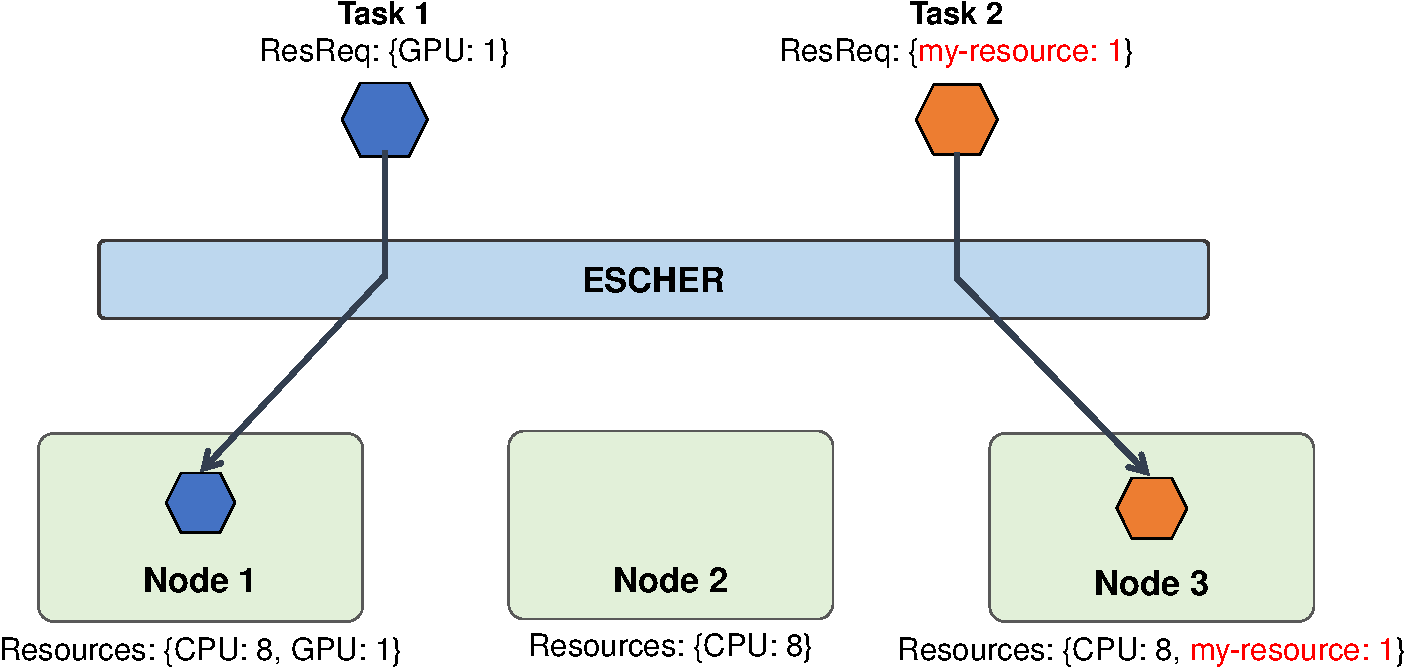
\includegraphics[width=\linewidth]{escher/figures/logicalres_demo.pdf}
%     \caption{An example demonstrating the use of ephemeral resources for targeted task placement. Applications can create custom resources, such as \emph{my-resource}, on the nodes where they wish to place a task, and then launch a task requesting \emph{my-resource} to ensure the task is placed on the desired node.}
%     %  Assuming a minimalist framework scheduler that matches task resource requests to node resource availabilities,
%     \label{fig:er-example}
% \end{figure}


% The key idea behind \name{} is then to leverage this scheduler functionality for a new type of resource: an \emph{ephemeral resource}. An ephemeral resource is a logical (i.e., non-physical) resource attribute that the application can dynamically associate with a node. The scheduler treats an ephemeral resource like any other physical resource, and aims to satisfy its capacity constraints. By associating an ephemeral resource with a particular physical node, the application can make targeted  placement decisions. As illustrated in Figure~\ref{fig:er-example}, creating a resource \lstinline{my-resource} on a node and then submitting a task requiring the resource \lstinline{my-resource} would result in the scheduler placing the task on 
% the node with enough capacity for \lstinline{my-resource}, assuming all other resource requirements are satisfied.
% Ephemeral resources follow the end-to-end argument, separating scheduling into two components: the application implements the policy, while the scheduler implements resource management.\swang{do we need this sentence? in general, a lot of this paragraph feels repetitive}
% % Surprisingly, many popular scheduling policies can be expressed in just a few lines of code using this simple mechanism, as demonstrated in Section \ref{policies}. 

% The remaining challenges in using ephemeral resources are then to: (1) generalize ephemeral resources to common policies, as well as new policies not expressible in monolithic systems today (\Cref{policies}), and (2) reduce burden for those applications that require standard policies or compositions thereof, while maintaining compatibility with more complex policies with fine-grained, dynamic scheduling decisions~(\Cref{sec:esl}).

% Why do this
% Using ephemeral resources to express scheduling constraints has several advantages. 




% Implementing the above policy is challenging because of two reasons. First, affinity and anti-affinity are conflicting requirements and therefore require an explicit specification of conflict resolution policies. Second, while the above policy can be naturally expressed as an hierarchical composition of simple policies (e.g., load-balance jobs across nodes, and co-locate all tasks of a job on the same node), very few cluster schedulers\cite{kubernetes} support such a composition. Worse, this support has limited flexibility and is restricted to a fixed set of policies. For instance, Kubernetes provides a scoring mechanism to assign weights between 13 policies, including affinity and anti-affinity policies. Moreover, these 13 policies do not constitute an exhaustive set of policies required by applications, such as gang scheduling.  %However, these policies cannot be modified by applications and custom policies cannot be integrated in the scoring computation without modifying the Kubernetes core. 
%there is no easy way to express this policy in existing cluster schedulers - they lack the primitives to adequately describe the policy. % For instance, Kubernetes \cite{kubernetes} provides a scoring mechanism to assign weights between affinity and anti-affinity policies, but does not allow a dynamic adjustment of  % \rliaw{the fundamental limitation of policy expression is not clear from the intro.}. 

% As a result, a new specialized scheduler, Gandiva~\cite{gandiva}, has been recently proposed to implement this policy. In addition to providing support for affinity and anti-affinity, Gandiva also implements job migration to help with resource de-fragmentation, i.e., consolidate small jobs on a subset of nodes to leave full nodes available to larger jobs.

% Not only sharing a cluster across multiple training jobs requires building a new scheduler, such as Gandiva, but once built, such a scheduler is not easy to extend. Currently, Gandiva is limited to distributed training jobs that fit on a single multi-GPU node. Thus, one natural extension is supporting distributed training on multiple nodes through gang scheduling. However, this is fundamentally challenging as the existing scheduler already maintains multiple state variables and checks for affinity, anti-affinity and job migration. Adding a gang-scheduling policy would require careful manipulation of this state and adding multiple constraints to satisfy all scheduling requirements. This greatly increases the complexity of the scheduler code and the functionality still remains to be added in the Gandiva scheduler. 

%This requires Gandiva to add support for gang scheduling, that is, run all tasks of the same job across multiple nodes simultaneously. Unfortunately, extending the existing Gandiva scheduler to support gang scheduling has proven  difficult~\cite{personal-communications}, and this functionality still remains to be added. 
%This illustrates the point that even trying to extend a scheduler to support a slightly more general workload is far from trivial.

% \subsection{Reinforcement Learning}

% \rliaw{could use figure here}
% Recently, reinforcement learning (RL) has led to breakthroughs in developing agents that exceed the human capabilities in playing computer games~\cite{dqn}, chess, and go~\cite{silver2016alphago}. As discussed in~\cite{ray}, implementing RL requires a system that support not only training, but model serving, and large scale simulations. Like in the case of Gandiva, this requires supporting a variety of policies: gang scheduling for multi-node distributed training and serving, anti-affinity (load balancing) to evenly distribute the simulations across the cluster, and affinity to run the tasks belonging to the same simulation on the same node. 

% Again, in the absence of cluster schedulers to support these policies simultaneously, researchers were left with no option but to implement specialized systems to support RL applications~\cite{gorila,evolution-strategy,ray}.


\section{ESCHER Design and Workflow}
\label{sec:arch}


% Express in three variables - Resource time and spatial.
A scheduling policy is defined by a set of temporal and spatial dependencies between tasks and nodes. We call these dependencies \emph{scheduling constraints}. 
%More precisely, scheduling constraints specify "when" and "where" (i.e., on which node) should a set of tasks be executed. Given the set of all tasks $W$, a scheduler must provide a schedule in the form of a one-to-many mapping of $S_t$ from $W$ to resources $R$ over all instants of time $T$.
%\[S_t: W \rightarrow R \quad \forall t \in T \]
The key idea in \name{} is to map these scheduling constraints to resource requirements by introducing a new resource type, \emph{ephemeral resources}.

 An ephemeral resource is a logical (i.e., non-physical) resource attribute that the application can dynamically associate with a node. Like physical resources, ephemeral resources have an associated capacity and can be acquired and released by tasks. 
We call these resources \emph{ephemeral} because the application can create, modify, and destroy them at runtime.
% This is in contrast to most existing frameworks, in which logical resources can only be created by framework operators~\cite{mesos,omega,yarn} and had been traditionally used to identify specialized hardware (e.g. TPUs). 

\name{} uses ephemeral resources for implementing scheduling constraints by leveraging a common functionality provided by cluster schedulers: matching the application-specified resource requirements with the cluster's resource availability. For instance, if an application task requires two GPUs, the scheduler should schedule that task on a node that has at least two available GPUs. With this resource-matching capability, the scheduler treats an ephemeral resource like a physical resource and aims to satisfy its capacity constraints.

The implementation of scheduling policies in \name{} follows a two-step pattern. First, the application creates ephemeral resources or updates capacities of existing ephemeral resources. This is done programmatically at runtime through the ephemeral resource API. Second, the application associates ephemeral resource requirements with tasks.
Note that these steps can happen in any order.
This allows the application to make targeted placement decisions (Figure~\ref{fig:er-example}) to satisfy the policy's scheduling constraints.

\begin{figure}[t]
    \centering
    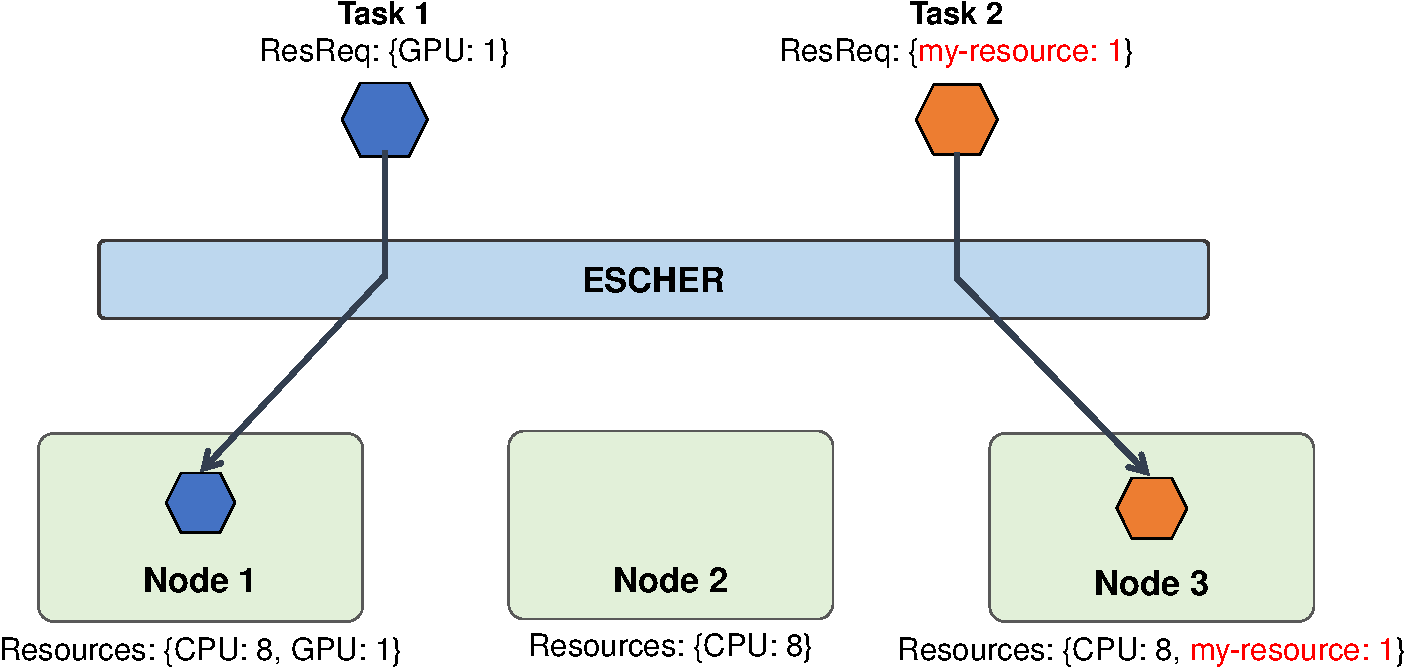
\includegraphics[width=0.92\linewidth]{escher/figures/logicalres_demo.pdf}
    \caption{\small Example using ephemeral resources for task placement. Applications create ephemeral resources (\emph{my-resource}) on the nodes where they wish to place a task and then launch a task requesting \emph{my-resource}. The resource-matching scheduler ensures the task is placed on the desired node.}
    %  Assuming a minimalist framework scheduler that matches task resource requests to node resource availabilities,
    \label{fig:er-example}
    \vspace{-4mm}
\end{figure}

\subsection{ESCHER Workflow}
\label{sec:arch:design}

Figure~\ref{fig:esl-arch} describes the workings of an ESCHER scheduler. %, the main components of the scheduler design, and the workflow between them. 
\name{} functionality, by design, is split between the application and the resource management framework.
The application can specify scheduling policies through the ephemeral resource API (\Cref{sec:arch:api}), while the framework performs resource matching and accounting over a set of underlying physical resources.
%The framework also exposes the two ESCHER API calls, \lstinline{set_resource} and \lstinline{get_cluster_state}, to allow ephemeral resource manipulation.
We envision that most applications would specify and compose policies through the higher-level \name{} Scheduling Library~(ESL) interface, which uses the ephemeral resource API to encapsulate common policies.

%% describe a typical workflow pattern
When using ESLs, an interaction with the system typically starts with an application requesting a scheduling policy from the ESL (\cref{fig:esl-arch}).
%The ESL implements the policy by creating the appropriate ephemeral resources in the resource manager.
The ESL may interact with the resource manager, e.g., by reading cluster state, and implements the policy by creating the appropriate ephemeral resources.
The application then receives a resource specification $R$ from the ESL.
The application attaches $R$ to a task and submits it to the resource manager for placement.

\subsection{Ephemeral Resource API}
\label{sec:arch:api}

\begin{sloppypar}
In \name{}, the resource management framework exposes two simple API calls to manage ephemeral resources: \lstinline{set_resource} and \lstinline{get_cluster_status} (Listing~\ref{list:er-api}). Once created, an ephemeral resource behaves as any regular physical resource and can be acquired and released by tasks.
\end{sloppypar}

In addition to the required parameters resource label and capacity, the \lstinline{set_resource} call also allows the specification of constraints \lstinline{node_spec} where the resource must be created. If \lstinline{node_spec} is a resource vector, the resource is updated on all nodes where the constraint resource vector is a subset of the node's available resource vector.
Optionally, a \lstinline{num_nodes} field in the \lstinline{node_spec} can specify how many nodes to execute \lstinline{set_resource} on if multiple nodes satisfy the \lstinline{node_spec} constraints.
To make targeted \lstinline{set_resource} calls, the \lstinline{node_spec} can contain a unique node identifier (e.g., IP address).

The \lstinline{get_cluster_status} call returns a mapping of node to local resource capacity and availability.
These are not required for all policies, but can be useful to handle node additions and removals~(\Cref{sec:esl-faulttol}).

% \textbf{Scheduler responsibilities.}
The ESCHER scheduler's responsibility is to provide the minimal guarantees provided by any resource-matching scheduler: (1) A task whose resource requirements can be met by a node in the cluster will eventually be scheduled, and (2) A node is never allocated past its capacity.
Together, these imply that the scheduler implements: (1) task queuing and dispatch, (2) node selection for each task, and (3) resource allocation for each task.
Note that the scheduler does not need to satisfy any other constraints, such as a promise regarding the node where a task is actually scheduled.

% \swang{cut} The key difference between \name{}'s API and the APIs of existing schedulers is giving applications the ability to create and manage (ephemeral) resources at runtime. With most existing frameworks \cite{mesos,omega,yarn}, resources can be only created by operators. Also, these resources are typically created before the framework is instantiated and do not change over the lifetime of the framework. 


\begin{figure}[t]
    \centering
     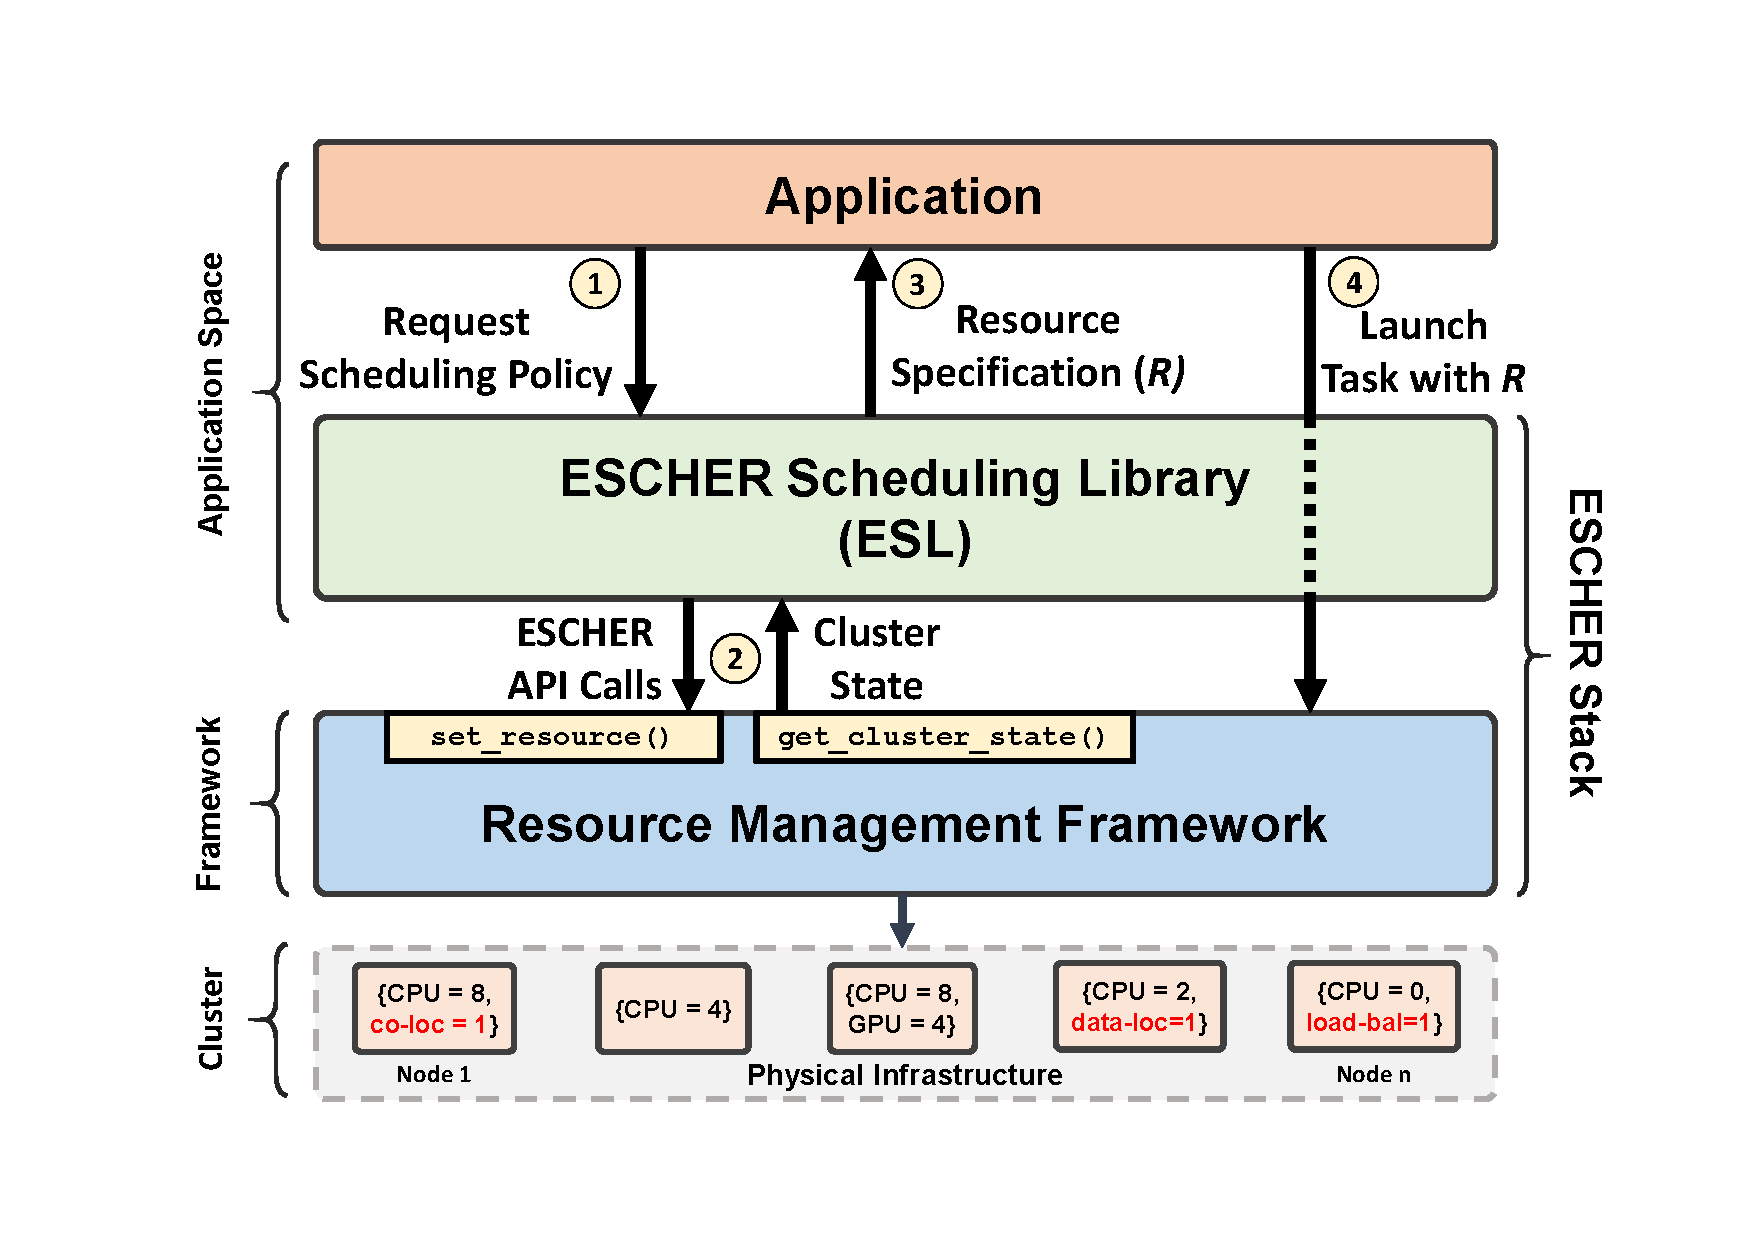
\includegraphics[width=0.95\linewidth]{escher/figures/idea_esl_arch.pdf}
    \caption{
        \small ESCHER task submission workflow with an ESL mediating the implementation. A task requests a supported scheduling policy from the ESL, which invokes the ESCHER API if necessary and returns the resource specification which would satisfy the policy. The task is launched with the returned resource specification.
    }
    \label{fig:esl-arch}
    \vspace{-2mm}
\end{figure}


\subsection{ESLs - \name{} Scheduling Libraries}   % Pronounced "Easel"
\label{sec:esl}

Controlling task placement through direct manipulation of ephemeral resources can be burdensome for applications with conventional scheduling requirements. 
%While the ESCHER API grants flexibility to applications to compose arbitrary scheduling policies, it requires applications to maintain ephemeral resource state and handle resource specification for tasks.
To reduce the application complexity and delineate scheduling policies from the mechanisms to implement them, we propose ESCHER Scheduling Libraries (ESLs).

The role of an ESL is simple - given a set of tasks, generate and apply a set of ephemeral resource requirements on the tasks which satisfy the desired scheduling policy.
ESLs achieve this by encapsulating the state management for ephemeral resources and providing a unified API for implementing domain-specific scheduling policies.
An application requests a scheduling policy supported by an ESL, which then makes the appropriate ESCHER API calls and returns the resource specification the application must use to realize its desired policy. In our implementations, ESLs are designed as a daemon that can service scheduling requests made from a single or multiple applications. 

ESLs are similar in spirit to Library Operating Systems (LibOS~\cite{Kaashoek:1997:APF:268998.266644}) in the Exokernel~\cite{exokernel} design.
% Just like a Library OS acts as a simplifying layer encapsulating the complexity of direct resource management exposed by an Exokernel, ESLs promote clean design and enable scheduling policies to be shared across different applications on an ESCHER scheduler.
In the same way that a LibOS encapsulates the complexity of direct resource management exposed by an Exokernel, an ESL abstracts the policy implementation and enables sharing across different applications.
% ESLs promote clean design and code re-use by abstracting all ESCHER related resource state into a unified layer that can be shared with other applications.
Moreover, this design makes applications portable across different cluster frameworks, e.g., Ray vs. Kubernetes~(\Cref{sec:impl}), since ESLs separate the application policy from the application code.
Finally, ESLs can protect applications from invalid specification of ephemeral resources by validating resource requests before launching tasks.

Since distributed applications can have widely varying scheduling requirements, we anticipate the development of domain-specific ESLs which can strike a balance between generality and preserving domain-specific optimizations. As an example, we describe and implement an ESL for hierarchical max-min fair sharing in \Cref{policies:hfs} and \Cref{eval:hfs}. % For instance, an ESL for dataframe processing applications could support data locality and task co-location, while adding implicit data replication at the ESL layer to improve data locality. As an example, we describe and implement an ESL for hierarchical max-min fair sharing in \cref{policies:hfs} and \cref{eval:hfs}.

% \subsubsection{\romilc{Example ESL - Ray Placement Groups}}
% % How can I use ESLs? You can do affinity plus gangn scheduling with ESLs. Show how they can compose. 
% \romilc{Ray\cite{ray-osdi} utilizes ephemeral resources to implement a ESL called the placement groups API. Placement groups allow users to atomically reserve groups of resources across multiple nodes (i.e., gang scheduling). They can be then used to schedule Ray tasks and actors to be packed as close as possible for locality (PACK qualifier), or spread apart (SPREAD qualifier).}

% \romilc{Ray placement groups operate by creating bundles of resources which can be atomically reserved by tasks. These bundles are reserved by creating ephemeral resources which replace the physical resources with unique virtual instances which are unique to a specific task. In other words, once a placement group is created, the original physical resources are consumed by the placement group, and ephemeral resources are then consumed by the task. The ESL manages the lifecycle of these ephemeral resources by creating them when tasks request a placement group and releasing them when the task ends.}

% \romilc{\romil{Fault tolerance?}If nodes that contain some bundles of a placement group die, all the bundles will be rescheduled on different nodes by Ray using the ephemeral resource API. This means that the initial creation of placement group is “atomic”, but once it is created, there could be partial placement groups.}


\begin{listing}
\begin{minted}{python}
# Create resource with name and capacity on a node 
# where the 'node_spec' constraints are satisfied.
# node_spec can be a resource vector or node id.
# If node_spec = None, resource is set locally
def set_resource(name, capacity, node_spec)

# Returns cluster resource state as a list of 
# node-wise map of local resource availability.
def get_cluster_status()
\end{minted}
\caption{Ephemeral resource API}
\vspace{-1em}
\label{list:er-api}
\end{listing}

\subsection{Fault tolerance}
\label{sec:esl-faulttol}
In the event of a node failure, ESCHER works in tandem with the fault-tolerance scheme of the underlying framework. Most frameworks~\cite{ray-osdi,kubernetes} simply re-execute the tasks with the same resource requirement. However, since these resource requests include ephemeral resources which no longer exist, these re-executed tasks cannot be scheduled.

At the bare minimum, an ESL must ensure that ephemeral resources are restored at some other eligible node. To do this, ESCHER relies on the cluster framework to report failed nodes through the \lstinline{get_cluster_status} API. Once failed nodes are detected, an ESL can recreate the ephemeral resources on suitable nodes by replaying the \lstinline{set_resource} calls for the failed resources. If a candidate node is found, the resource is recreated, else the tasks must wait for the failed node to recover before they can be rescheduled. When a node is restored, its resources are also reinitialized, allowing any waiting tasks to get rescheduled. % In addition to this basic policy, ESLs can define application-specific recovery routines.% after the ephemeral resources are restored.

\subsection{Evolvability and complexity in \name{}}
\label{sec:arch:evolve}
The ability to create ephemeral resources on targeted nodes makes scheduling with ESCHER as flexible as letting the application directly
control task placement on cluster nodes. %schedule its tasks on any node in the cluster. 
Indeed, scheduling a task $T$ on node $N$ is equivalent to assigning a uniquely-named ephemeral resource $R_N$ with capacity 1 to node $N$, and having $T$ request one unit of resource $R_N$. 


% Should this go in related work
While this targeted placement makes ESCHER highly evolvable, what are its benefits over simply
yielding placement control over resources to the application directly?
% giving the application direct access to the cluster's resources? 
After all, if the goal is to schedule a task on a particular node, ESCHER makes this operation arguably more complex as it requires creating an ephemeral resource on the node.% to place the task there.

The primary benefit of ESCHER is that policy and ESL implementations do not need to reason about \emph{tasks}.
In a framework with fully application-level scheduling, such as Mesos or Omega \cite{mesos, omega}, the application scheduler has to maintain possibly distributed state about the current set of tasks.
When a task is submitted and can't yet be scheduled, the scheduler queues the task.
When a task starts, the scheduler must update the current resource availability to ensure that resources do not become oversubscribed.
On task completion, the scheduler must again update the current resource availability and select a new task to run from the queue.

Of course, none of these functionalities are unique to ESCHER.
Task to resource matching is a necessity to every scheduler system, which is why it is the core responsibility that we assign to the ESCHER scheduler.
Thus, in ESCHER, \emph{an application that has no specific policy requirements can use an ESCHER scheduler directly without implementing any scheduling code}.
This is not possible in systems that expose resources directly to the application, such as Mesos~\cite{mesos} or Omega~\cite{omega}, as it is expected that the application will also implement all mechanisms related to task scheduling.

For applications that do require a custom policy or an ESL, this division of responsibilities still reduces the effort required from the application developer, compared to implementing a complete scheduler.
For example, most of the policies that we present in \Cref{tab:escher-constraints-policies} do not require examining the current cluster state; it is enough for a task to create a resource on its local node or create resources on all nodes that match a given resource spec.
The exceptions are gang scheduling, which requires reading the cluster state to roll back a group of tasks in case of a failure, and load-balancing, which computes the current load from the cluster state.
In contrast, a fully application-level scheduler must continually update and reason about the current cluster state in order to find a suitable node for each task.
In the ESCHER design, this responsibility is given to the system rather than the application.
%\camready{ESLs don’t concern themselves with physical resource allocation, only consumption and creation of ephemeral resources.}

% ESCHER provides three key benefits over exposing the cluster’s resources to the application.
% %and letting the application implement scheduling policies from scratch. 
% \textbf{[R1]} First, it offers a single source of the global resource availability truth. %of the nodes across the cluster. 
% In the absence of this mechanism, it's up to each individual application to do so. This is problematic for many reasons.
% Local application's view of resources must be maintained on start/completion of each resource consuming task and each resource-bearing node arrival/departure. This requires each application to be fault-aware.
% % If we just expose the cluster’s resources to the application, the application needs to keep track of the cluster’s resource availability itself. In particular, when a task starts or finishes, the application needs to update the node’s resource availability. Furthermore, the application needs to update this availability as nodes fail, which means it needs to detect failures. 

% \textbf{[R2]} Second, distributed application resource state tracking/management can easily lead to resource coordination failures  potentially causing deadlocks. When multiple applications maintain their local view of the same shared resource availability state, maintaining consistency of this state in a distributed system is a complex problem, especially in the presence of node and task failures. This requires implementation of expensive distributed consensus protocols or optimistic concurrency mechanisms (e.g., Omega~\cite{omega}). Surprisingly, even with proper distributed resource state management, applications may still enter livelock situations when they incrementally request resources to satisfy complex constraints, such as gang scheduling constraints (e.g., Mesos~\cite{mesos}).
% % Finally, if there are multiple applications sharing the same cluster they have to somehow share the availability state. This is a complex problem as it reduces to maintaining the consistency of the state (i.e., node resource availability) in a distributed system in the presence of failures. 

% \textbf{[R3]} Third, ephemeral resources enable applications to naturally express an exhaustive family of scheduling constraints. 
% We consider scheduling constraints of three types: 
% (a) \textbf{spatial}: a \textit{where} constraint on resource properties required for task placement (e.g., GPUs, CPU architecture, memory, availability of executable binaries~\cite{bikash-google-socc11});
% (b) \textbf{temporal}: a \textit{when} constraint on the relative ordering of tasks with respect to each other. Examples include gang scheduling (temporally simultaneous). 
% (c) \textbf{task-task}: constraints irrespective of the physical properties of underlying resources or time. These include constraints or preferences on the virtual task topology, e.g., Scheduling a directed acyclic graph (DAG) of tasks.
% %with clusters of tasks exhibiting structural coupling within tasks in each cluster and loose coupling across the clusters. Scheduling a directed acyclic graph (DAG) of tasks is another distinct class of task-task constraints. 
% The ``happens-before'' relationship between tasks is notoriously difficult to express declaratively (e.g., not supported by state-of-the-art DCM~\cite{dcm-osdi20} and TetriSched~\cite{tetrisched}) and requires specialized imperative heuristics, sacrificing both evolvability and generality (e.g., Spark DAG Scheduler~\cite{spark-dagscheduler}).
% Fundamentally, ESCHER's dynamic ephemeral resources serve as a \textit{reduction mechanism}, reducing both, task-task constraints to spatial or temporal, and temporal constraints to spatial. We exemplify this novel reduction mechanism in Table~\ref{tab:escher-constraints-policies}.

% define \textit{a scheduling constraint} as a constraint on resource properties required for task placement (spatial) or a constraint on the ordering of tasks relative to each other (temporal). Examples incl
% By \textit{scheduling constraints} we mean any constraint imposed on scheduling two or more tasks, such as running two tasks at the same time (i.e., gang scheduling), co-locating two tasks (i.e., affinity) and co-locating data with computation (i.e., locality-aware scheduling). In particular, \name{} enables applications to cast scheduling constraints as ephemeral resource constraints, and then lets its resource-constrained scheduler enforce these constraints. For example, to implement locality-aware scheduling, an application can assign to each data item a uniquely-named ephemeral resource and then add the ephemeral resource associated with a task’s input to its resource requirements. \name{} does the rest. If a data item is replicated on multiple nodes, this solution works without any changes; just assign the same ephemeral resource to every node storing a replica of the data item. In contrast, if we just expose the cluster resources to the application, the application will need to keep track of the mapping between data items and nodes storing these data items, which again reduces to maintaining the state consistent in a distributed system.
\section{Scheduling with \name{}}
\label{policies}

%\input{policy-table-v2.tex}

% In this section, we first describe a taxonomy of scheduling policies (\cref{policies:taxonomy}) then show examples of how an application can use ephemeral resources to implement a variety of policies~(\Cref{policies:example1,policies:example2}, \Cref{fig:policycode}), including composite policies~(\Cref{policies:composition}) and policies with soft constraints~(\Cref{softconstr}).


% \subsection{Casting policies as resource requirements}
% \label{policies:taxonomy}

%In this section, we describe how applications can use \name{} to implement scheduling policies.
A scheduling policy is a mapping of tasks to resources which satisfies any spatial ("where") and temporal ("when") constraints.
%These constraints can be spatial (\textit{where} a task must run) or temporal (\textit{when} a task must run). Spatial constraints specify the exact node where a task must run and temporal constraints specify a time dependency between tasks.
We now describe how these constraints can be cast as resource requirements with \name{}. % Since \lstinline{set_resource} allows the creation of ephemeral resources on any node, even the most complex spatial constraint can be expressed by explicitly creating ephemeral resources on a targeted node. Since ephemeral resources are dynamic, temporal constraints can be expressed by modifying ephemeral resources at runtime.
%For instance, creating a simple temporal dependency between two tasks $T_1$ and $T_2$ can be expressed by having task $T_1$ create an ephemeral resource $X$ when it completes, and requesting resource $X$ in task $T_2$'s resource requirements.

%Given the set of all tasks $W$, a scheduler must provide a schedule in the form of a one-to-many mapping of $S_t$ from $W$ to resources $R$ over all instants of time $T$.
%\[S_t: W \rightarrow R \quad \forall t \in T \]

\begin{table*}[t]
\small
\begin{threeparttable}
\begin{tabular}{|p{3.75cm}|p{2.5cm}|p{10.25cm}|}
\hline
\textbf{Policy Example}                            & \textbf{Primitive used}                  & \textbf{Implementation with ESCHER}                                 \\ \hline
\textbf{Sequential}: Run $T_2$ after $T_1$.         & Signaling                         & $T_2$ requests ephemeral resource $E$ created by $T_1$ on completion. %creates an ephemeral resource $E$ when it finishes. $T_2$ requests $E$. 
\\ \hline
\textbf{Gang Scheduling}: Run $T_1$ and $T_2$ simultaneously.      & Locking, Signaling                         & Two ghost tasks $T_1^g$ and $T_2^g$ request 1 CPU each, and each creates an ephemeral resource $E_{CPU}$ of capacity one. When both $T_1^g$ and $T_2^g$ run, schedule $T_1$ and $T_2$, each requesting one unit of $E_{CPU}$. \\ \hline
\textbf{Affinity}: Run $T_1$ and $T_2$ on the same node.           & Locality                         & A ghost task $T^g$ requests 2 CPUs, and creates an ephemeral resource $E$ with capacity 2. $T_1$ and $T_2$ request one unit of $E$ each. \\ \hline
\textbf{Anti-affinity}: Run $T_1$ and $T_2$ on different nodes.    & Queues                         &  Every node in the cluster creates anti-affinity resource $E$ with capacity 1.  $T_1$ and $T_2$ request one unit of $E$ each.\tnote{1} \\ \hline
\textbf{Load-balancing}: Evenly spread tasks across nodes.           & Queues                         & Create load-balancing resource $L$ with capacity 1 on each node. Each task requests one unit of $L$ each. When all $L$ resources are exhausted, increase capacity by 1. \\ \hline
\textbf{Data-locality}: Run $T$ where its input $D$ is stored. & Locality                         & When storing $D$, create ephemeral resource $E_D$ on the same node. $T$ requests $E_D$. \\ \hline
\end{tabular}
\begin{tablenotes}\footnotesize
\item [1] If $T_1$ and $T_2$ are long-running, the application cannot use the nodes they are running on for other anti-affinity placements. To avoid this, we have two short-lived ghost tasks $T_1^g$ and $T_2^g$ request 1 unit of $E$ each, create ephemeral resources $E_1$ and $E_2$, and then terminate. $T_1$ requests $E_1$ and $T_2$ requests $E_2$.
\end{tablenotes}
\caption{Expressing scheduling constraints with ephemeral resources}
\vspace{-1em}
\label{tab:escher-constraints-policies}
\end{threeparttable}
\end{table*}

\subsection{Scheduling primitives in ESCHER}
\label{sec:sched:primitive}
We present four scheduling primitives implemented using ephemeral resources which can be used to express both spatial and temporal constraints. We note that this is not an exhaustive set of primitives possible with ephemeral resources. Applications have the flexibility to define their own primitives through ephemeral resource manipulation.

\textbf{[P1] Locality.} 
Tasks must often be co-scheduled on the same physical node as another task or must be co-located with data. These spatial constraints can be easily expressed in ESCHER. The target task for co-location creates a local ephemeral resource $E_r$ with unbounded capacity when the task starts or the data to be co-located with is created. The constrained task then requests 1 unit of $E_r$ and, thus, automatically gets scheduled on the same node.

\textbf{[P2] Task Signaling.}
Distributed applications rely on expensive RPCs to coordinate the execution of interdependent tasks. This is prevalent in directed acyclic graph~(DAG) task schedulers, where the ordering of tasks is critical for correctness. These temporal constraints can be expressed with ESCHER by creating ephemeral resources dynamically, effectively using them as signals. E.g., if task T2 has \textit{any} ``happens-before'' dependency on task T1, T1 can create a resource $E_{T2}$ when it completes. T2 \textit{a priori} requests $E_{T2}$ as a part of its resource requirements when launched, and thus is scheduled as soon as $E_{T2}$ is created by T1.  Note that signals in ESCHER are single-shot---all task requests are declaratively placed at the start, and tasks begin execution only when their ephemeral resource demands are met by newly created resources. 
% It is notable that T1 can create $E_{T2}$ at any point of its execution, making ephemeral resources expressive enough to initiate logically dependent task T2 before T1 completes, but no sooner than is deemed safe by T1.
More generally, barrier synchronization is naturally supported. Given $\left\{ T^{i-1}_j \right\} \rightarrow T^i$ for $j>1$, $T^i$ could simply request a single unit of resource created by each of $T^{i-1}_j$ upon their respective completion. Thus, semaphores (and therefore, mutual exclusion) can also be implemented. % with ephemeral resources.

\textbf{[P3] Queues.}
Many policies \cite{wfq, sfs} use one or more task queues as a fundamental construct in their implementation. 
The core ESCHER scheduler queues tasks until their resource requirements (ephemeral and physical) can be satisfied. ESCHER allows the application to decide when to dequeue tasks by increasing the capacity of an ephemeral resource. 
% orts task queues by design, since tasks whose resource requirements (ephemeral and physical) are not satisfied are queued in the scheduler till they are feasible. Thus, 
Creating a queue is simply creating a unique ephemeral resource $E_q$ with initial capacity 0 on any node. A task is enqueued by launching it in a wrapper task requesting 1 unit of $E_q$ resource. The queue drain rate can be set by changing the capacity of $E_q$. On acquiring the $E_q$ resource, the wrapper task submits the contained task to the scheduler with its physical resource requirement (e.g., 2 CPUs) and exits. Note that it's possible to implement batched scheduling %with dynamically adjustable mini-batch size
 by incrementing the capacity of $E_q$ by the desired batch size.

\textbf{[P4] Resource Locking.}
ESCHER enables a new scheduling construct where an ephemeral resource can be used to acquire and lock one or more physical resources ("bundle"). This reservation of resources is achieved with \emph{ghost tasks} - long-running tasks which acquire the bundle like a regular task and create a local ephemeral resource to accommodate new tasks. Ghost tasks create a pattern of indirection where tasks request ephemeral resources instead of physical resources to get scheduled. We note that ghost tasks achieve the same outcome as incremental locking presented in Omega~\cite{omega}. This is useful when applications require atomic transactions on a \emph{group} of resources, such as in gang scheduling.


% \subsection{Application Policy: Load Balancing}
% \label{policies:example1}
% Consider a simple policy such as elastic load balancing. In some applications, such as web servers, it is desirable to evenly spread out tasks to minimize the average load per node and eliminate single points of failure. Moreover, the bursty nature of these workloads, where the exact number of requests to be served is not known, adds dynamicity to the scheduling requirement.

% \begin{sloppypar}
% To implement this spatial constraint, ephemeral resources can provide load balancing by creating a resource \lstinline{load_balancer} on each node and having each incoming task request 1 unit of this \lstinline{load_balancer} resource. To make this policy scale with incoming tasks, a separate \lstinline{load_monitor} process continually monitors the state of the \lstinline{load_balancer} resource on all nodes and increments it all nodes are equally occupied or decrements it if all nodes have more than one available \lstinline{load_balancer} resource. By performing these two functions, the \lstinline{load_monitor} task ensures that the resource availability remains elastic, and thus every task requesting the \lstinline{load_balancer} resource gets scheduled evenly across all nodes.
% \end{sloppypar}

\subsection{Scheduling policies with ESCHER}
\label{policies:gangsched}
\label{sec:sched:policies}
To illustrate the use of these scheduling primitive constructs, we now describe the implementation of an example application-level policy and a cluster-level policy with ESCHER. \Cref{tab:escher-constraints-policies} lists more policies and their implementation with \name{}.

\subsubsection{Application Policy: Gang Scheduling}
Distributed training \cite{gandiva} and reinforcement learning workloads~\cite{gorila} require gang scheduling, where all tasks should start and run concurrently. This implies all-or-none scheduling semantics, where either all resources requested by all tasks are granted simultaneously, or no resources are granted.

In implementing all-or-none constraints, a common requirement is to check whether sufficient resources are available to satisfy the policy and reserving them, if necessary.
%For instance, gang-scheduling requires a fixed size pool of resources to be available to tasks.
To achieve this, \name{} uses \textit{ghost tasks} from the resource locking primitive. 
For instance, gang-scheduling a pool of 8 tasks (each of which requires 1 CPU) can be done by launching a ghost task which requires 8 CPUs and creates 8 units of \lstinline{gang-sched} resource. If all ghost tasks are successful, each task in the pool can then request 1 \lstinline{gang-sched} resource and 0 CPUs to get scheduled. If any ghost task is unsuccessful, a timeout in other ghost tasks executes a rollback and removes the \lstinline{gang-sched} resource. To avoid live-locks, either the applications can execute an exponential back-off \cite{expbackoff} before retrying, or an ESL can serialize all gang scheduling requests through a common shared library. We discuss this design space in \Cref{sec:eval:gangscheduling}.

%Gang scheduling can be implemented with ephemeral resources by creating reservation tasks that are submitted with the same resource requirements as the actual tasks, as demonstrated in Figure \ref{fig:policycode:gangsched}. On instantiation, all reservation tasks create a \lstinline{reservation} resource of capacity 1 on their host node and send a heartbeat to the application. The receipt of heartbeats from all reservation tasks indicates a successful resource acquisition and the application can then launch the gang of tasks by having each task request one unit of the \lstinline{reservation} resource each. If the opportunistic scheduling of reservation task fails (identified by a timeout), the reservation tasks remove the \lstinline{reservation} resource and terminate.

\begin{figure}[t]
\centering
%% Fig A
% \begin{subfigure}[b]{0.33\linewidth}
%   \centering
%   \begin{subfigure}{\textwidth}
% \begin{minted}[fontsize=\scriptsize]{python}
% esl = HFS(domain=cluster.nodes())
% res_user_a = esl.create_user("a", 1)
% res_user_b = esl.create_user("b", 2)

% # User A's code
% task.launch(resources={res_user_a: 1})

% # User B's code
% task.launch(resources={res_user_b: 1})
% \end{minted}
% \end{subfigure}
%   \caption{}
%   \label{listing:eslexample}
% \end{subfigure}
%% Fig b

\begin{subfigure}[b]{0.45\linewidth}
  \centering
  \begin{subfigure}{\textwidth}
\begin{minted}[fontsize=\tiny]{python}
def soft_constraint_scheduler(task, ordinal_resource_preferences):
  for res_pref in ordinal_resource_preferences:
    if recv_heartbeat(task.task_id):
      break
    task.resources = res_pref
    task.launch()
    sleep(timeout)

def main():
  res_prefs = [{gpu: 1}, {cpu: 1}]
  soft_constraint_scheduler(task, res_prefs)
\end{minted}
\end{subfigure}
  \caption{}
  \label{listing:softconstr}
\end{subfigure}
%% Fig c
\begin{subfigure}[b]{0.45\linewidth}
  \centering
  \begin{subfigure}{\textwidth}
\begin{minted}[fontsize=\tiny]{python}
def task1(id):
  set_resource(label=id, capacity=1)
  ...
def composite_scheduling():
  # Create load-balancing resources
  for node in cluster:
    set_resource("load_balancing", 1, node)
  for i in range(0, task_count):
    # Load balance task 1
    task1.launch(id=i, resources = {'load_balancing': 1})
    # Co-locate task 1 & 2
    task2.launch(resources = {i: 1})
\end{minted}
\end{subfigure}
  \caption{}
  \label{listing:compositionpolicy}
\end{subfigure}

\caption{\small Scheduling with \name{}. \textbf{(a)} Soft constraints with \name{}. \textbf{(b)} Composition of load-balancing and co-location policies with ephemeral resources in \name{}.}
\label{fig:schedpseudo2}
\vspace{-5mm}
\end{figure}

\subsubsection{Cluster Policy: Hierarchical Fair Sharing}
\label{policies:hfs}
From a cluster operator's perspective, using ESCHER allows enforcement of cluster-level scheduling goals, such as multi-tenancy, while still supporting application-level scheduling policies described above. For example, consider large organizations, which typically have a cluster of resources shared among teams. This sharing has three requirements. First, the scheduler must allow assigning resource sharing weights to users. Second, to maximize resource utilization, the scheduler must implement max-min fairness~\cite{ghodsi2011dominant}, i.e., temporarily re-allocate idle resources to oversubscribed users. Finally, teams  need to further partition their share of resources among sub-teams. % The scheduler must support creating hierarchies of max-min fair sharing.

Hierarchical max-min fair sharing (HFS) can be implemented as an ESL using a variant of the Queue primitive. The HFS ESL is instantiated to operate on a specified domain of nodes and provides a single call - \lstinline{create_user(id, weight)} - which returns a resource name unique to the user id. On invoking this routine, the ESL executes a \lstinline{set_resource} call to create a unique resource (e.g., \lstinline{res_user1}) with infinite capacity for the user on each allocated node. When a user submits a task, they must request a capacity of 1 their unique resource label (e.g., \lstinline{res_user1}) which ensures their task is run only on the resources provisioned for them.  Since ephemeral resources can be updated at runtime, the ESL dynamically resizes user allocations by adding and removing their ephemeral resources. Hierarchies in this setup can be created by launching multiple instances of the ESL  and restricting their operating domain to the nodes granted by the parent ESL.

%To achieve max-min fairness, the HFS ESL implements a lending scheme which runs a daemon to monitor the users' resource utilization through the \lstinline{get_cluster_status} call. If any user's available resource capacity is zero (i.e., the user is oversubscribed), the ESL first tries to reclaim any resources this user may have lent to other users. If no borrowers are found, the user borrows resources from other users who have available resource capacity (i.e., are undersubscribed).

\subsubsection{Soft constraints with ESCHER}
\label{sec:softconstraints}
The core scheduler enforces task resource requirements as a hard constraint, keeping the core scheduling logic simple. %a strict matching of task resource requirements to cluster resource availability.
% If any resource in the set of requirements is unavailable, scheduling will fail even if other resources are available.
However, some applications may demand relaxed scheduling semantics, where some resource requirements can be specified as \textit{soft constraints}.
% If the soft constraints are not satisfied, they can be discarded and the task is rescheduled with only the remaining resource requirements.
Ephemeral resources can be used to implement soft constraints even when the scheduler only supports strict matching of resource requirements.
First, the application specifies the soft constraints as an ordinal set of resource set preferences $R = [r_1, r_2, ..., r_n]$, where $r_i$ is the $i^{th}$ preferred resource requirement set.
% The ordering of this set indicates the resource preference order.
For instance, an application which prefers a GPU but will work without one would specify its resource requirements as $R = [\{gpu: 1\}, \{\} ]$.

The soft-constraints ESL then instruments the application's tasks with a lightweight heartbeat sent to the ESL to notify it of successful scheduling when the task launches (Listing \ref{listing:softconstr}).
The ESL then sequentially attempts to launch a task, starting with resource requirement $r_1$. If the ESL does not receive the callback from the task within a certain timeout $t$, it implies the resource requirement was not matched.
The ESL then cancels and resubmits the task, now with a resource requirement $r_2$. This best-effort scheduling is attempted for all resource preferences $r \in R$ until the scheduling succeeds or all preferences have been evaluated.

% This mechanism also prevents any duplicate execution of tasks. The response to a task heartbeat is a signal which indicates if the task should continue execution or terminate immediately. When a task successfully launches for the first time, the application sends a continue execution signal, but any subsequent successful task heartbeats are sent the termination signal. This ensures that any duplicate launches, either due to resources becoming available over time or a short wait timeout, are suppressed.

%NOTE(romilb):Ephermerality of resources isn't really used for soft-constraints..

% \begin{listing}
% \begin{minted}[fontsize=\tiny]{python}
% def task():
%   is_valid_run = send_heartbeat()
%   if is_valid_run:
%     ...

% def soft_constraint_scheduler(task, ordinal_resource_preferences):
%   for resource_preference in ordinal_resource_preferences:
%     if heartbeat_already_received(task.task_id):
%       break
%     task.resources = resource_preference
%     task.launch()
%     sleep(timeout)

% def main():
%   ordinal_resource_preferences = [{gpu: 1}, {cpu: 1}]
%   soft_constraint_scheduler(task, ordinal_resource_preferences)
% \end{minted}
% \caption{Soft constraints with \name{}}
% \label{listing:softconstr}
% \end{listing}

% % Code figure
\newcommand\colmult{0.23}
\begin{figure*}[t]
~
% Task co-location
~
\begin{subfigure}[b]{\colmult \textwidth}
  \centering
  \begin{minted}[fontsize=\tiny,breaksymbolleft=\tiny\ensuremath{},breakautoindent=true]{python}
def task_colocation():
 constraint = sum([t.resources for t in coloc_tasks])
 set_resource("co-grp", len(coloc_tasks), constraint)
 for task in coloc_tasks:
  task.launch(res={"co-grp": 1})
  \end{minted}
  \caption{Task Co-location}
  \label{fig:policycode:taskcoloc}
\end{subfigure}
~
% Data locality TODO: Consider showing task based data locality too.
~
\begin{subfigure}[b]{\colmult\textwidth}
  \centering
  \begin{minted}[fontsize=\tiny,breaksymbolleft=\tiny\ensuremath{},stripnl=false]{python}
def data_locality():
  data_addr = get_location(data)  # Node id
  set_resource("data-loc", 1, data_addr)
  task.launch(res={"data-loc": 1})
  
  
  \end{minted}
  \caption{Data locality}
  \label{fig:policycode:datalocality}
\end{subfigure}
~
% Policy: Anti Affinity
~
\begin{subfigure}[b]{\colmult\textwidth}
  \centering
  \begin{minted}[fontsize=\tiny,breaksymbolleft=\tiny\ensuremath{},stripnl=false]{python}
def anti_affinity():
  for node in nodes:
    set_resource("anti_aff", 1, node)
  for task in anti_affinity_tasks:
    task.launch(res={"anti_aff": 1})

  \end{minted}
  \caption{Anti-affinity}
  \label{fig:policycode:antiaff}
\end{subfigure}
~
% Static Load Balancing
~
\begin{subfigure}[b]{\colmult\textwidth}
  \centering
  \begin{minted}[fontsize=\tiny,breaksymbolleft=\tiny\ensuremath{}]{python}
def static_load_bal():
 cap = ceiling(num_tasks/num_nodes)
 for node in nodes:
  set_resource("load_bal", cap, node)
 for task in tasks:
  task.launch(res={"load_bal": 1})
  \end{minted}
  \caption{Static Load Balancing}
  \label{fig:policycode:staticloadbal}
\end{subfigure}

\newline
\vspace{2.0mm}

~
% Dynamic Load Balancing
~
\begin{subfigure}[b]{\colmult\textwidth}
  \centering
  \begin{minted}[fontsize=\tiny,breaksymbolleft=\tiny\ensuremath{}]{python}
def load_monitor():
 while True:
  res = get_cluster_status()
  if res["load_bal"] == 0 on all nodes:
   set_resource("load_bal", increment 1, all_nodes)
  if res["load_bal"] >= 1 on all nodes:
   set_resource("load_bal", decrement 1, all_nodes)
def dynamic_load_bal():
  task.launch(res={"load_bal": 1})
  \end{minted}
% for task in tasks:
%   task.resources = {"load_bal": 1}
%   task.launch()
  \caption{Dynamic Load Balancing}
  \label{fig:policycode:dynloadbal}
\end{subfigure}
~
% Policy: Binpacking
~
\begin{subfigure}[b]{\colmult\textwidth}
  \centering
  \begin{minted}[fontsize=\tiny,breaksymbolleft=\tiny\ensuremath{},stripnl=false,escapeinside=||,mathescape=true]{python}
def expand_binpack_nodes(res):
 find node where node.resources > res:
  set_resource("binpack", |$\infty$|, node)


def binpacking():
  cluster_res = get_cluster_status()
  if task_res is not subset(binpack_nodes):
    expand_binpack_nodes(task_res)
  task.launch(res={"binpack": 1})
  
  
  \end{minted}
  \caption{Bin-packing}
  \label{fig:policycode:binpacking}
\end{subfigure}
~
% Policy: Gang sched
~
\begin{subfigure}[b]{\colmult\textwidth}
  \centering
  \begin{minted}[fontsize=\tiny,breaksymbolleft=\tiny\ensuremath{}]{python}
def ghost_task(child_tasks, timeout):
  set_resource("reserved", len(child_tasks))
  wait(child_tasks, timeout)
  set_resource("reserved", 0)

def gang_scheduling():
 ghost_task(gang_tasks).launch(res = sum(task_resreqs))
 for t in gang_tasks: 
   t.launch(res={"reserved": 1})
  \end{minted}
  \caption{Gang Scheduling}
  \label{fig:policycode:gangsched}
\end{subfigure}

\caption{Implementation of popular scheduling policies with ephemeral resources. \name{} can allow locality based policies by creating ephemeral resources on nodes which can satisfy the said locality. \name{} can also be used to implement dynamic policies such as load-balancing and bin-packing by implementing lightweight processes which can adjust ephemeral resource capacities on the fly.}
\label{fig:policycode}
\end{figure*}

\label{policies:objective}
\textbf{Objective functions.}
Soft constraints can be used to approximate policies that optimize a combined objective function.
% In addition to spatial and temporal scheduling policies, ephemeral resources can also be used to approximate policies which aim to optimize on a combined objective function.
For instance, consider a policy which aims to balance both CPU and memory utilization in a cluster.
% load balance tasks on a weighted function of CPU and memory availability.
Formally, given weights for memory and CPU utilization $\alpha$ and $\beta$, the objective is to maximize the minimum of $\gamma_n=\alpha M_n + \beta C_n$ across all nodes, where $M_n$ and $C_n$ are the memory and CPU utilization on node $n$ (ranging between 0 and 1).

% Mathematically, given the set of all nodes in the cluster $N$ and weights for memory and CPU availability $\alpha$ and $\beta$, the objective is to:
% {\small
% %\vspace{-12pt}
% \begin{equation}
% \max\min_{\forall n \in N} (\alpha\text{$MEM_n$} + \beta\text{$CPU_n$})
% \end{equation}
% }
% where $MEM_n$ and $CPU_n$ are CPU availability values (ranging between 0 to 1) on node $n$. It is possible to approximate such maxmin optimization policies with ESCHER.
To express this policy in ESCHER, the scheduler first creates the resource \textit{obj} on each node with a capacity of $\alpha+\beta$.
A task with memory and CPU requirements $m$ and $n$ then specifies the soft constraint $R = [\{obj: \gamma\}, \{obj: \frac{\gamma}{2}\}, \{obj: \frac{\gamma}{4}\},... \{obj: \frac{\gamma}{2^k}\}]$, where $\gamma = \alpha m + \beta n$.
The task also includes the hard constraints $\{MEM: m, CPU: n\}$.
This preference places each task on the least utilized node, correct up to a factor of 2, while guaranteeing that no node is overallocated.

% To run tasks, each task uses soft constraints to specify a resource set preference of $R = [\{obj: \gamma\}, \{obj: \frac{\gamma}{2}\}, \{obj: \frac{\gamma}{4}\},... \{obj: \frac{\gamma}{2^k}\}]$. Such a resource set preference allows each task to be placed on the least utilized node, correct upto a factor of 2. On successful scheduling, the task calls \lstinline{set_resource} on the local \textit{obj} resource to signal its consumption and reduce its quantity.

% Note that this approach may incur significant overheads from repeated retries when the resources are oversubscribed. As an alternative, this policy can also be implemented by observing the cluster state, computing the objective function locally and using targeted placement with \lstinline{set_resource} to directly place the task on the desired node. \romil{TODO: We need to politely admit that this solution is a bit too complex/has overheads.}


\subsubsection{Policy Composition}
%\label{policies:composition}
%TODO(romilb): Add graphic to explain this better?
% Some applications may have scheduling requirements that may be expressed as a hierarchical composition of the basic scheduling policies discussed above. For instance, an application might want to enforce co-location among a set of tasks, while evenly spreading out these groups of co-located tasks to load balance across the cluster. Implementing this policy on existing frameworks is challenging due to the highly specific needs of this application. Even if the application developer was to modify the core framework scheduler, the implementation of this policy is still complex, requiring significant developer effort to develop and maintain.
Applications like hyperparameter search require a hierarchical composition of other policies~(\Cref{sec:motivation:example}).
% With ephemeral resources a hierarchical policy can be easily expressed as a composition of other policies.
Scheduling policy compositions can be logically expressed either as an AND conjunction or an OR conjunction. AND constraints are expressed by concatenating the ephemeral resource vectors for two policies. OR constraints are supported using soft constraints. % An OR composition of two policies P1 and P2 can be specified as the ordinal set [\{P1, P2\}, \{P1\}, \{P2\}].}
For instance, if an application wants to co-locate $task1$ and $task2$ while load balancing their groups across the cluster, it can simply apply co-location on $task1$ and $task2$ and load balancing only on $task1$ as shown in \cref{listing:compositionpolicy}. Similarly, cluster-level policies can be composed with application-level policies (Section \ref{eval:hfs}). 

Conflicting compositions of policies may render a task impossible to schedule. E.g., composing a cluster-level fair sharing policy and an anti-affinity policy may result in a infeasible task if the fair share  of resources is insufficient. In such situations, one can specify conflict resolutions by using soft-constraints to relax scheduling policies. For instance, a soft constraint vector [\{\text{fair\_a: 1}, \text{anti\_aff: 1}\}, \{\text{fair\_a: 1}\}] would try scheduling a task with fairness and anti-affinity, and relax the anti-affinity constraint if a conflict arises. 

% \begin{listing}
% \begin{minted}[fontsize=\tiny]{python}
% def task1(id):
%   set_resource(label=id, capacity=1)
%   ...
% def task2():
%   ...
% def composite_scheduling():
%   # Create load-balancing resources
%   for node in cluster:
%     set_resource("load_balancing", 1, node)
%   # Launch tasks
%   for i in range(0, task_count):
%     # Load balance task 1
%     task1.launch(id=i, resources = {'load_balancing': 1})
%     # Co-locate task 1 & 2
%     task2.launch(resources = {i: 1})
% \end{minted}
% \caption{Composition of load-balancing and co-location policies with ephemeral resources in \name{}.}
% \label{compositionpolicy}
% \end{listing}

% \subsection{Custom application policies}
% \romil{Candidate for cutting}
% The ephemeral resource abstraction also enables expression of custom application policies.
% For instance, consider a data-locality sensitive application~\cite{clipper} serving multiple replicas of a periodically retrained machine learning model. Such models can be hundreds of megabytes in size, so instantiating new model actor replicas for inference is best done on the node where a cached copy of the model can be found. However, the application also requires continuous updates to the model, which can result in stale caches of the model across the cluster. \name{} allows easy invalidation of caches when the base model is retrained by simply setting the capacity of the \lstinline{data-locality} (Figure \ref{fig:policycode:datalocality}) resource to zero on nodes where the model is stale, and resetting it to one when the cache is updated.

% Similarly, the use of ephemeral resources enables single-shot task-to-task affinity scheduling. While task-to-node affinity can be achieved in other schedulers as well~\cite{tetrisched,firmament}, task-to-task affinity is more difficult to express in such schedulers because it is relative to other units of compute, not relative to physical nodes. \name{} makes it possible to submit all affine tasks at once, e.g., without waiting for the first task to complete before submitting other tasks. Tasks stay pending internally until \textit{co\_location} ephemeral resource creation succeeds, after which all affine tasks get scheduled. 
%\section{ESLs - \name{} Scheduling Libraries}   % Pronounced "Easel"
\label{sec:esl}

%Describe the problem - application code and programmer must deal with cumbersome resource management
% Controlling task placement through direct manipulation of ephemeral resources can be burdensome for applications with conventional scheduling requirements. While ESCHER grants flexibility to applications to compose arbitrary scheduling policies through combinations of resource constraints, it requires applications to maintain resource state and handle low-level resource specification for tasks. This resource specification can become particularly intricate when multiple scheduling policies must be composed. Moreover, many applications, such as MapReduce\cite{mapreduce} and dataframe\cite{DevinMasters} processing, share common scheduling objectives and can have a shared policy implementation.
Controlling task placement through direct manipulation of ephemeral resources can be burdensome for applications with conventional scheduling requirements. While the ESCHER API grants flexibility to applications to compose arbitrary scheduling policies
%through combinations of resource constraints
, it requires applications to maintain ephemeral resource state and handle resource specification for tasks. % This resource specification can become particularly intricate when multiple scheduling policies must be composed. Moreover, many applications, such as MapReduce\cite{mapreduce} and dataframe\cite{DevinMasters} processing, share common scheduling objectives and can have a shared policy implementation.
To reduce the application complexity and delineate scheduling policies from the mechanisms to implement them, we propose ESCHER Scheduling Libraries (ESLs).

ESLs are similar in spirit to Library Operating Systems (LibOS,~\cite{Kaashoek:1997:APF:268998.266644}) in the Exokernel\cite{exokernel} design.
% Just like a Library OS acts as a simplifying layer encapsulating the complexity of direct resource management exposed by an Exokernel, ESLs promote clean design and enable scheduling policies to be shared across different applications on an ESCHER scheduler.
In the same way that a LibOS encapsulates the complexity of direct resource management exposed by an Exokernel, an ESL abstracts the policy implementation and enables sharing across different \name{} applications.
% ESLs promote clean design and code re-use by abstracting all ESCHER related resource state into a unified layer that can be shared with other applications.
Moreover, this design makes applications portable across different cluster frameworks, e.g., Ray vs. Kubernetes~(\Cref{sec:impl}), since ESLs separate the application policy from the application code.
Finally, ESLs can optionally protect applications from invalid specification of ephemeral resource requests by verifying the consistency of resource requests using the \lstinline{get_cluster_state} call before launching the task.

% \begin{figure}[ht]
%     \centering
%     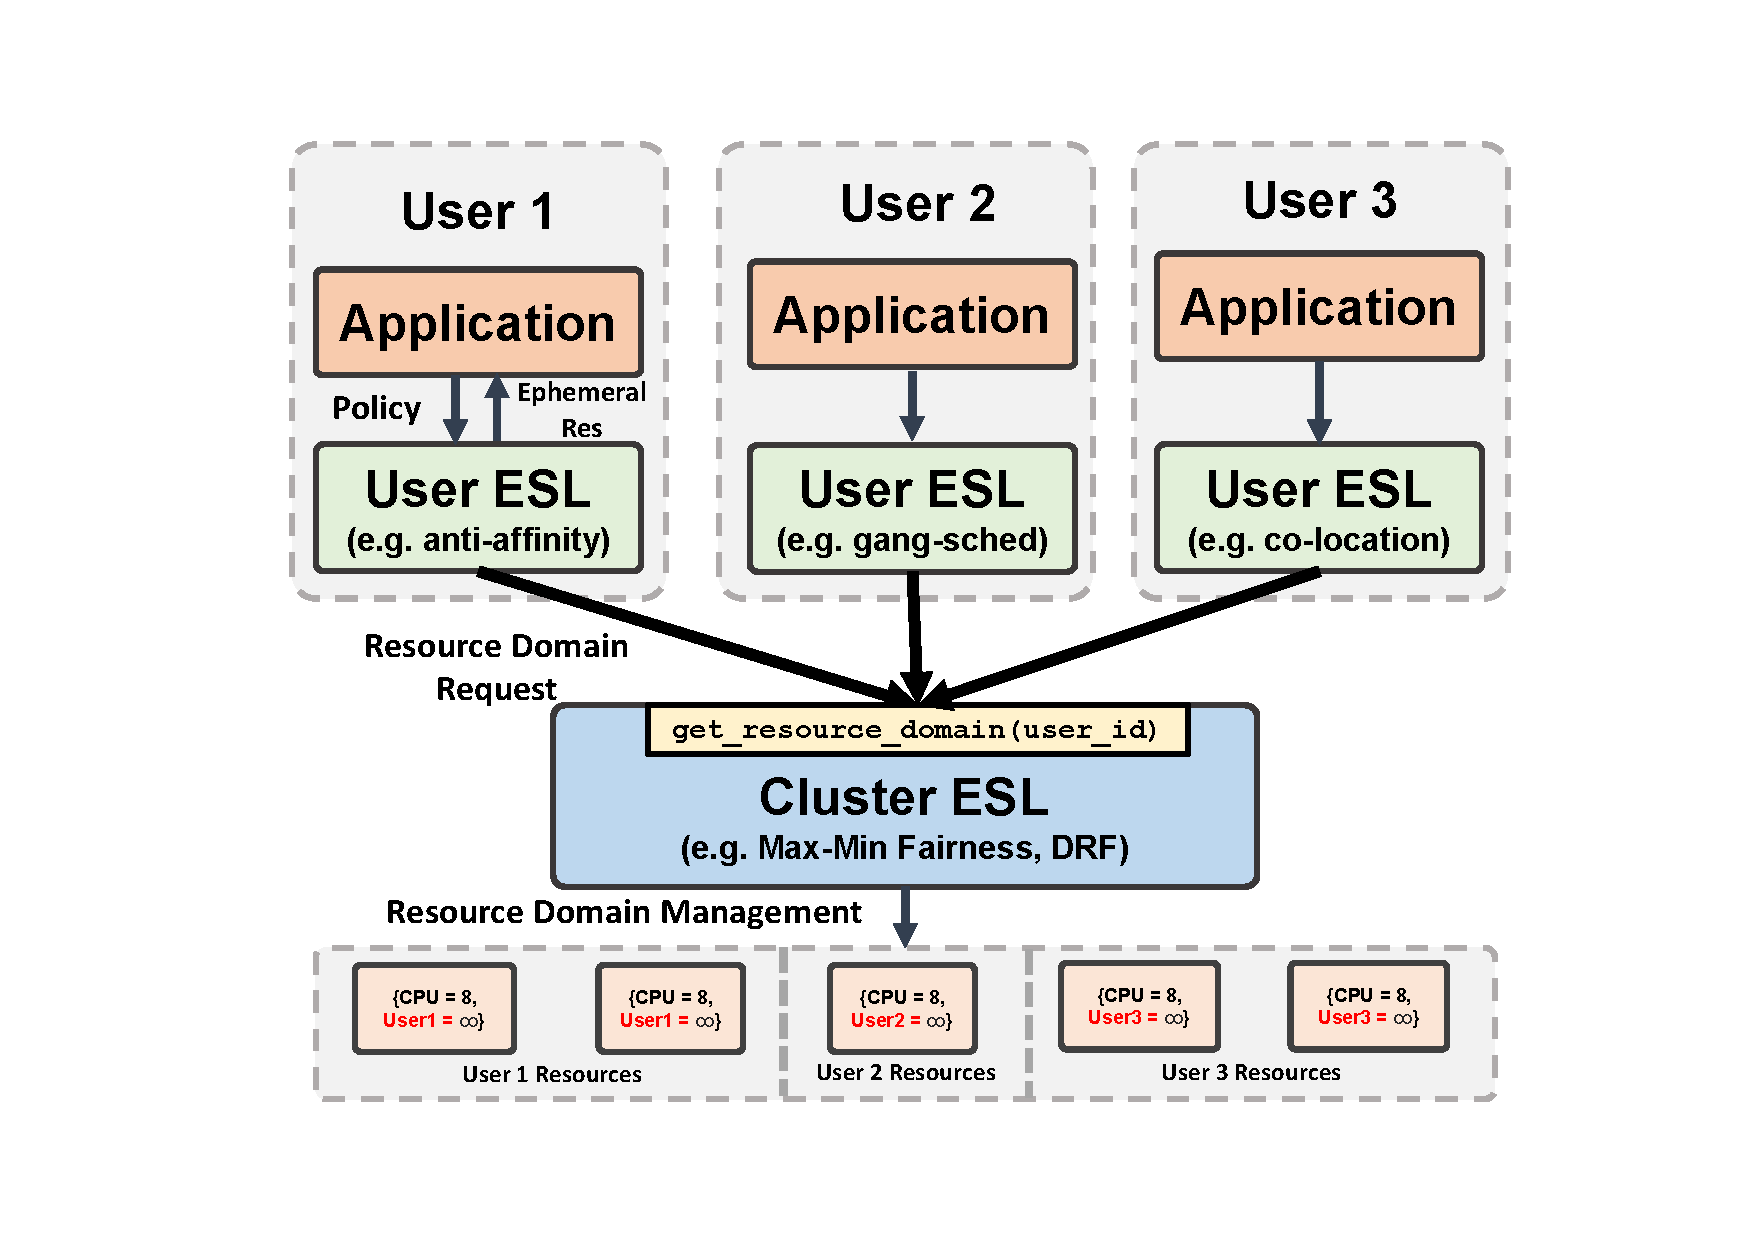
\includegraphics[width=\linewidth]{escher/figures/clusteresl_useresl.pdf}
%     \caption{
%         \small Isolation mechanisms in ESCHER. To avoid resource conflicts between ESLs, ESCHER uses a two-layer design to isolate applications. A cluster ESL provides a resource domain (a set of nodes) to each user's application-level ESLs. This resource domain is dynamically adjusted by the cluster ESL's policy. The resource domain restricts a user ESL from creating resources outside their authorized pool. 
%     }
%     \label{fig:esl-isolation}
%     %\vspace{-4mm}
% \end{figure}

\subsection{ESL Design}
An ESL encapsulates the state management for ephemeral resources and provides a unified API for implementing domain-specific scheduling policies. An application requests one of the many high level scheduling policies supported by an ESL, which then makes the appropriate ESCHER API calls and returns the exact resource specification the application should use to realize its desired policy. In our implementations, ESLs are designed as a daemon that can service scheduling requests made from a single or multiple applications.

 % Figure \ref{fig:esl-arch} describes the workflow to use an ESL. An application first initializes it or connects to a pre-existing ESL which implements the desired scheduling policy. It then makes a ESL specific call to select the policy and any related parameters (such as co-location group name, or minimum slots for gang scheduling). The ESL inspects the cluster state and invokes the \lstinline{set_resource()} API to update ephemeral resources if required. Finally, it returns the exact resource specification the task must use to satisfy the requested policy. This resource specification can be used as-is or further concatenated with with other resource specifications to compose custom policies.

Since distributed applications can have widely varying scheduling requirements, we anticipate the development of domain-specific ESLs which can strike a balance between generality and preserving low-level domain-specific optimizations. For instance, an ESL for dataframe processing applications could support data locality and task co-location, while adding implicit data-replication at the ESL layer to improve data locality. 

% Design - Explain the figure and how applications still have resource control if required. 2 Phase protocol for task submission.
\begin{sloppypar}
As an example, we illustrate a big-data ESL to encapsulate two popular policies --- data locality and task co-location. This ESL exposes two methods to applications: \lstinline[breaklines=true]{get_coloc_group(group_name, node_resources)} and \lstinline[breaklines=true]{get_dataloc_group(data_id)}. 
%\swang{no reference to get\_dataloc\_group in the listing?} fixed.
These methods allow an application to create logical locality groups in the ESL and get the resource specification which would place tasks in locality group. Internally, ESL maintains the state related to locality groups and implements the policies as described in Section \ref{policies}. Listing \ref{listing:eslexample} illustrates how an application interacts with the big-data ESL.
\end{sloppypar}

\begin{listing}
\begin{minted}{python}
esl = BigDataESL()
coloc_res = esl.get_colocation_group("mygroup", node_resources={gpu: 8})
dataloc_res = esl.get_dataloc_group(data_handle)

# Use ESL resource specification to co-locate tasks t1 and t2
# and enforce data locality for t3
t1.launch(resources+=coloc_res)
t2.launch(resources+=coloc_res)
t3.launch(resources+=dataloc_res)
\end{minted}
\caption{\small Using the big-data ESL to enforce task co-location. The ESL methods return a resource specification which is used to launch the co-located tasks.}
\label{listing:eslexample}
\end{listing}

% Comments - we anticipate domain specific scheduling libraries. ESLs are optional. 

% Benefits - Simplified application code, code resuse across applications, portability of applications, domain specific optimizations
% Moreover, using ESLs has four key benefits.
% \begin{itemize}
%     \item\textbf{Simplified Code:} The use of ESLs greatly simplifies application-level code since all ESCHER related resource state management is abstracted into a unified layer. 
%     \item\textbf{Code Re-use:} Applications performing similar tasks often have overlapping scheduling requirements. For instance, it is common for dataframe processing applications to require data locality. Instead of individually implementing data locality, all these applications could use instances a single ESL.
%     \item\textbf{Portability:} Exporting the policy implementation to the ESL makes applications portable across different cluster frameworks (such as Ray, Kubernetes) and updates to policy implementation can be pushed without affecting the application code.
%     \item\textbf{Resource specification safety:} Invalid specification of ephemeral resources due to stale resource state can render tasks unschedulable. ESLs can integrate resource safety checks which verify the consistency of resource requests using the \lstinline{get_cluster_state} call before launching the task.
%     %\item\textbf{Domain Specific Optimizations:} The use of ESLs allows domain specific optimizations like replication for datalocality
% \end{itemize}


\subsection{Fault tolerance}
\label{sec:esl-faulttol}
In the event of a node failure, ESCHER works in tandem with the fault-tolerance scheme of the underlying framework but also allows the application developers to specify custom fault-tolerance routines through an ESL. Most frameworks, including Ray\cite{ray-osdi} and Kubernetes\cite{kubernetes}, simply re-execute the tasks with the same resource requirement. However, since these resource requests include ephemeral resources which no longer exist, these re-executed tasks cannot be scheduled.

At the bare minimum, an ESL must ensure that ephemeral resources are restored at some other eligible node. To do this, ESCHER relies on the cluster framework to report failed nodes through the \lstinline{get_cluster_state} API. Once failed nodes are detected, an ESL can recreate the ephemeral resources on suitable nodes by replaying the \lstinline{set_resource} calls for the failed resources. If a candidate node is found, the resource is recreated, else the tasks must wait for the failed node to recover before they can be rescheduled. When a node is restored, it's resources are also reinitialized allowing any waiting tasks to get rescheduled. In addition to this basic policy, ESLs can define custom routines such as error reporting and logging after the ephemeral resources are restored.
\section{Implementation}
\label{sec:impl}
\name{} is a design that can be applied to both centralized and decentralized schedulers.
We built two prototypes of \name{}, on Kubernetes~\cite{kubernetes}, a container orchestration framework with a centralized scheduler, and Ray~\cite{ray}, a distributed execution framework with a decentralized scheduler.
% Similarly, ESCHER on Ray inherits Ray's sequential scheduling of queued tasks, but batch scheduling can be performed using the queuing primitive from Section \ref{sec:sched:primitive}.}

ESCHER inherits the scheduling properties of the parent cluster framework. For instance, it can utilize fractional and heterogeneous resources on Ray and Kubernetes. Since Ray and Kubernetes have a task-by-task scheduler, our current implementation also schedules in a greedy, task-by-task manner. However, ESCHER's queuing primitive can be used to extend a task-by-task scheduler to do batch scheduling.

Each framework handles isolation differently, which affects how ghost tasks are implemented. Ray does not enforce CPU affinity, so a ghost task can block the logical resource for the actual task without blocking the physical CPU. Kubernetes enforces isolation through cgroups. In this case, the ghost task reserves the CPU for its cgroup and when the actual task is scheduled, it is added to the same cgroup by running cgclassify in the task's preamble.
The source code is available at \href{https://github.com/romilbhardwaj/escher}{https://github.com/romilbhardwaj/escher}.
% \swang{strengthen the takeaway here: show that we can do it for existing schedulers, both centralized and decentralized}

\noindent\textbf{Kubernetes Implementation.}
% Describe the Kuberenetes scheduler's features and policies supported off-the-shelf
%Kubernetes is a cluster orchestration system designed for managing and deploying containers across machines.
%A task in Kubernetes comprises one or multiple containers grouped in a logical scheduling unit called a Pod.
A Kubernetes task (pod) specifies its constraints in the form of two sets: a set of filtering policies, such as resource demands, to enforce hard constraints and a set of weights for these built-in policies to add soft constraints.
%The filtering policies include resource capacity and node label checks which must necessarily be satisfied by the node where the Pod will be scheduled. The scoring policies specify good-to-have conditions such as inter-pod affinity and load balancing to achieve an priority ordering among multiple policies. 
The scheduler first finds a set of candidate nodes, then computes a policy-weighted score for each node to find the best fit.

Kubernetes also allows the definition of arbitrary string and integer pairs associated with nodes known as \textit{extended resources}. Extended resources are identical to regular resources in that they can be acquired and released by Pods, except they can be defined as arbitrary key value pairs.
The extended resources API has conventionally been used by cluster operators for marking specialized hardware as a one-time operation when the cluster is initialized. In fact, application pods are not granted access to this API by default.  

To implement the ESCHER \textit{set\_resource} API, we change the Kubernetes role-based access control to allow applications to directly invoke the extended resources API in Kubernetes. This grants applications the ability to create and update \textit{extended resources} using the \textit{patch\_node\_status} call.
From a security perspective, ESCHER applications require access only to create and remove extended resources. The Kubernetes API should deny write access to physical resources. Additionally, we employ namespacing of resources to enforce isolation and prevent malicious applications from overriding other applications.

To force the Kubernetes scheduler to act as a simple resource-matching scheduler, the scheduler is invoked with only hard resource constraints set in the filtering policy. Weights for all other policies are set to zero. Thus, the combination of \textit{extended resources} API with hard resource constraints makes it possible to implement ESCHER policies on Kubernetes \emph{without making any changes to the core Kubernetes scheduler}.
% Instead, we can repurpose existing APIs and scheduler modes in Kubernetes.
%It invokes the \textit{patch\_node\_status} method with an ADD operation on the node's resource set. If the resource does not exist, the ADD operation creates a resource, else updates the resource with the new capacity..

% Note that this implementation requires no changes to the core Kubernetes source. ESCHER's generality allows it to re-purpose existing APIs and scheduler modes in Kubernetes.

\noindent\textbf{Ray Implementation.}
Ray runs a scheduler per node, which collectively implement a bottom-up decentralized resource matching mechanism~\cite{ray}. Each node in the cluster has a set of key-value pairs signifying resource labels and their quantity, e.g., \texttt{\{"cpu": 8, "gpu": 1\}}.
Each task specifies its hard resource requirements with the same data structure.
% A task can only be executed on a node whose available resources are a superset of the task's resource requirement.

Ray nodes share a centralized log of the total resource capacity at each node, where each entry represents the capacity at a node.
% In addition, each node emits periodic heartbeats containing the node's current resource availability.
The Ray scheduler matches a task to resources by storing resource availabilities from other nodes in a map and allocating the first node which can satisfy the task's resource request.
Since a scheduler's view of the global state is only eventually consistent, it can correct previous decisions by running the same logic to find another eligible node. To support ESCHER, we extend the Ray core to permit updates to each node's resource capacity at runtime.
We restructure Ray's centralized log so that each entry stores only a \emph{delta}, instead of the absolute capacity at that node.
This guarantees no race conditions occur between resource updates, while avoiding expensive coordination, e.g., via a distributed lock.

% Ray runs one scheduler per node, which collectively implement a bottom-up distributed resource matching mechanism. Once a task enters this distributed scheduler, it is queued in the scheduler on some particular node. If the node's available resources exceed the task's resource requirements, the scheduler begins executing the task on that node. Otherwise, if a different node in the cluster has sufficient available resources to run the task, the task is forwarded to that node and the recipient node repeats the scheduling logic. If no node in the cluster has sufficient available resources to run the task, the task is queued at some node in the cluster until the required resources become available somewhere in the cluster.


%Each node in the Ray cluster is configured at startup with a set of resources. 
%Each resource is described with a name and capacity. The name, an arbitrary string, typically refers to specific hardware resources (e.g., ``cpu'', ``gpu''). Resource quantity is a positive scalar. Node resources are configured on startup and advertised when the node joins the cluster.
%Similarly, each Ray task specifies its hard resource requirements. These requirements are a set of resource names and the corresponding required quantities. A given task can only be executed on a node whose configured resources are a superset of the task's resource requirement. Furthermore, the sum of the resource requirements of % all tasks executing concurrently on any given node must be a subset of the node's configured resource capacity.

% Ray runs one scheduler per node, which collectively implement a bottom-up distributed resource matching mechanism. Once a task enters this distributed scheduler, it is queued in the scheduler on some particular node. If the node's available resources exceed the task's resource requirements, the scheduler begins executing the task on that node. Otherwise, if a different node in the cluster has sufficient available resources to run the task, the task is forwarded to that node and the recipient node repeats the scheduling logic (because each node has a stale view of each other node's available resources, it is possible that the relevant resources will no longer be available once the task arrives). If no node in the cluster has sufficient available resources to run the task, the task is queued at some node in the cluster until the required resources become available somewhere in the cluster.

%is responsible for scheduling tasks on that node. When a task is created by an application, it is queued in one of the schedulers. That scheduler may then forward the task to another scheduler, may assign it for execution on that scheduler's node, or may leave it queued. If at least one node in the cluster has sufficient available resource capacity to execute the given task, then the task will be forwarded to a node with sufficient capacity and executed.

%A task specification in Ray includes a resource vector, indicating the resources and their quantities required for the execution of the task. This resource vector is treated as a hard requirement and must be satisfied on the node where the task is scheduled. When a task is launched, it acquires the resources requested by it and releases them when the task is completed.

%The scheduler design in Ray builds on distributed resource matching scheme where each node runs a local scheduler with a simple logic - match tasks to nodes where the resources requested are available. If the local node has sufficient resources for the task, it runs on the local node, else gets forwarded to a remote node which can satisfy the task's resource requirement. The remote node then repeats the scheduling logic. Infeasible tasks which cannot be scheduled due to insufficient resources wait in a queue till all requested resources are available in the cluster. 

%\subsubsection{Dynamic resource state manipulation}
% While the Ray scheduler design satisfies the scheduling requirements in \Cref{sec:arch:ephres}, resource management in Ray does not permit resource modification and updates at runtime. We now discuss the Ray resource tracking mechanisms and the challenges in adding dynamic resource update support to the Ray resource management subsystem.

% For fault-tolerance and resource discovery, Ray maintains a centralized log of the total resource capacity available on each node. However, to make correct scheduling decisions, each per-node scheduler must have a real-time global view of the cluster resource utilization state. This is constructed by emitting periodic heartbeats from each node containing the node's real time resource state, which are consumed by other nodes to update their local view of the cluster state. Though this creates a loose but eventually consistent view, it does not adversely impact scheduler performance, since the heartbeat period is much smaller than an average task's lifespan. Even if a scheduler makes an incorrect decision, it gets corrected when the remote node re-runs the scheduling logic on the forwarded task.

% In such a distributed resource management paradigm, manipulating resources at runtime can be challenging. The complexity arises from propagating resource updates and maintaining consistency of the global state across schedulers. While heartbeats would update resource state on every node, state stored in the central log would also need to be updated. This gets challenging when multiple resources on the same node are updated concurrently, since out-of-order updates may violate the consistency of the log.

% A naive solution would be to enforce locks on the log, but that would negatively impact the resource update latency. Instead, we restructure the log to store only the diff of resource updates, called resource deltas. Since they are composed only of changes in resource capacities, resource deltas are commutative and their ordering in a log is inconsequential. This enables resource updates to be carried out without adding locks on the log. 

%Creating resources at runtime can be challenging for frameworks that utilize distributed schedulers. The complexity arises from propagating resource updates and maintaining consistency of the global state across schedulers without compromising on the scheduling latency. In our implementation, resource state is stored in a central log which grants a unified view of the cluster and provides desirable fault tolerance properties. To avoid head-of-line blocking and maintain a low scheduling latency, all schedulers maintain a local replica of this state and update it whenever a resource update occurs. However, instead of just storing the entire resource vector for every entry in the log, the framework must store only resource updates (deltas). This is to avoid dropping resource updates at the scheduler level because of out-of-order messages that update the node's entire resource vector may overwrite other updates. % Todo: Need to explain better/ remove this para.

\begin{figure*}[t]
\begin{subfigure}[b]{0.30\textwidth}
\centering
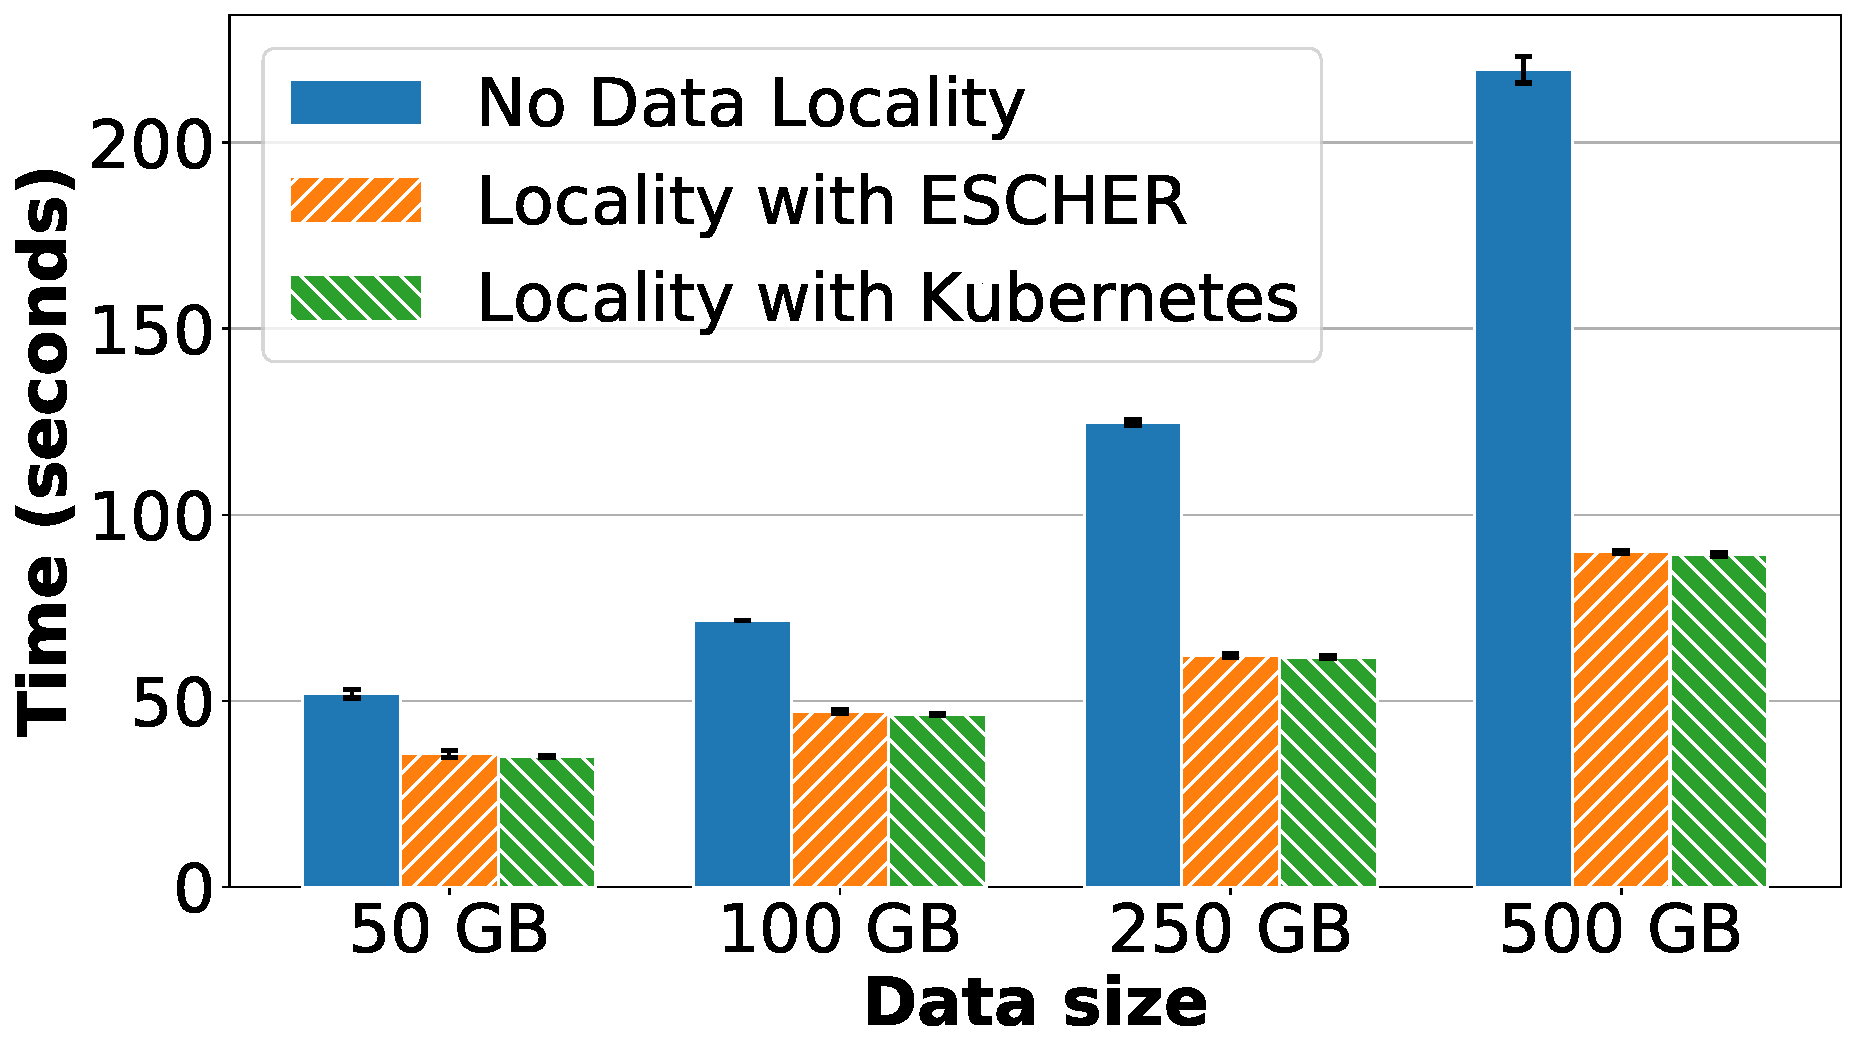
\includegraphics[width=\textwidth]{escher/plots/mapreduce_makespan.pdf}
\caption{
%A random placement policy has high network overheads due to poor data-locality. ESCHER implementation on Kubernetes performs comparably with the off-the-shelf core Kubernetes data locality policy.
}
\label{fig:mapreduce-makespan}
\end{subfigure}
\begin{subfigure}[b]{0.39\textwidth}
\hspace{2mm}
\footnotesize
% \begin{table}[ht]
% \begin{center}
\raisebox{15mm}{
\begin{tabular}{cccc}
% {\tiny
\toprule
& \multicolumn{3}{c}{\textbf{Scheduler}}\\
\textbf{Nodes}     & Generic & Kubernetes & ESCHER \\
\midrule
10 & $183.32 \pm 0.51$ & $54.69 \pm 0.46$ & $55.24 \pm 0.39$ \\\hline
50 & $113.71 \pm 0.49$ & $44.02 \pm 0.27$ & $44.71 \pm 0.44$  \\\hline
100 & $51.90 \pm 0.31$ & $35.08 \pm 0.31$ & $35.76 \pm 0.49$  \\
\bottomrule
% }
\end{tabular}
}
\caption{
% As the cluster size increases, ESCHER scales similarly to core kubernetes scheduler, while outperforming the generic data-locality unaware scheduler.
}
\label{tab:mapreduce-xnode}
%\vspace{-8mm}
% \end{table}
\end{subfigure}
\begin{subfigure}[b]{0.30\textwidth}
 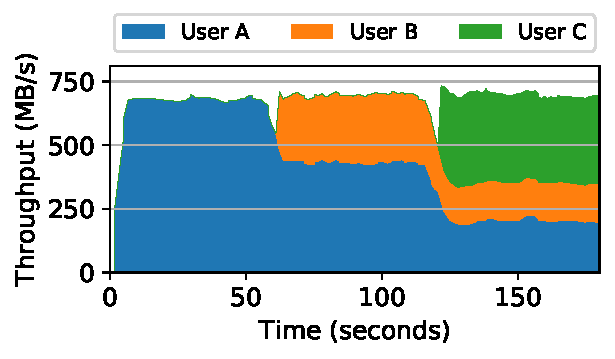
\includegraphics[width=\textwidth]{escher/plots/hfs/3user_hfs_sharing_mapreduce_50nodes_area_short.pdf}
 \caption{}
 \label{fig:hfs-3user-result}
\end{subfigure}
\vspace{-2em}
\caption{\small 
Data locality and hierarchical max-min fair sharing for WordCount.
\textbf{(a)} Makespan of WordCount running on a 100-node Kubernetes cluster, comparing a random placement policy, ESCHER on Kubernetes with data locality, and Kubernetes' native data locality.
\textbf{(b)} Makespan of WordCount MapReduce jobs in seconds across varying cluster sizes.
\textbf{(c)} Hierarchical max-min fair sharing with ESCHER.
A and B are in Sub-Org1 with weights 2:3; C is in Sub-Org2.
A, B, and C begin submitting tasks at $t=$0, 60, and 120, respectively.
}
\vspace{-3mm}
\end{figure*}


\section{Evaluation}
\label{sec:eval}

In this section, we evaluate the following questions:
\begin{compactitem}
    \item Can existing distributed applications be ported to use ESCHER and what are its implications?
    \item What are the tradeoffs with implementing scheduling policies in the application space vs in the framework?
    \item What are the overheads of scheduling with ephemeral resources?
\end{compactitem}

All evaluations use Amazon EC2 m5.12xlarge, m5.4xlarge or p3.8xlarge instances. Kubernetes clusters are provisioned using Amazon EKS running version 1.19.

\subsection{End-to-end Evaluation}
\label{sec:eval:e2e}
% Logical resources act as a thin layer of scheduling indirection for applications without sacrificing framework flexibility.
%In this section, we study four applications and their scheduling requirements. We then demonstrate how \name{} can accelerate these applications by allowing them to express complex scheduling policies with minimal developer effort.

\subsubsection{WordCount with MapReduce}
\label{eval:wordcount}
% What is mapreduce, what is word count
%These chunks are then individually processed by multiple mapper tasks in a distributed fashion. The results of mapper tasks are consumed by reduce tasks which key-wise consolidate the results.
WordCount counts the number of words in large text datasets and is often implemented with MapReduce~\cite{mapreduce}. To avoid expensive data transfers, data locality is essential.
% A data locality policy is essential to performance in this model, since map tasks must be colocated with their assigned inputs (which are usually on disk at a particular node) to avoid expensive data transfers.
% WordCount is a program implemented on the MapReduce~\cite{mapreduce} model to count the number of words in large text datasets. WordCount works by splitting the text file into smaller chunks, distributing them over the network and then running distributed mappers to count word frequency in these chunks.
% How data locality plays in. Implementation, HDFS Spark etc.
% The map tasks in WordCount are highly dependent on their locality with the data chunk they are assigned to process. If the data chunk is not present on the node where the map task is scheduled, it is forced to perform an expensive fetch over the network before starting processing. This dependence makes WordCount a benchmark to stress data-locality.
% Describe setup 100 nodes.
We implement the map and reduce tasks as independent operators running in containers.
The input files are chunks of a file with random words, each hosted by one of 100 nodes. The total input size is varied from 50 GB to 500 GB.
% and use Kubernetes to distribute these tasks over a 100-node cluster.
% The inputs are chunks of a file with random words, each  hosted by one of 100 nodes. 
% The total input size is varied from 50 GB to 500 GB.
%In this setup, the scheduler must place the mapper tasks on the nodes which host their chunk to minimize delays from network transfers.
We implement \name{} on Kubernetes, using an ESL for data locality (\Cref{policies}), and compare against Kubernetes's built-in data-locality policy~\cite{kubernetes-doc} and a locality-unaware random policy.
% For \name{} on Kubernetes, we use an ESL that implements data locality (\Cref{policies}).

% How do it in k8s, ESCHER.
% To achieve this data locality with the default Kubernetes scheduler, we use the \lstinline{NodeAffinityPriority} specifier in the scheduler to place mappers on nodes where their assigned chunk exists. This serves as a baseline to compares against ESCHER. In ESCHER, we create a resource \lstinline{chunk-n} on each node, where $n$ is the id of chunk hosted by the node. The mappers then request this resource to get co-located with their chunk. This policy is wrapped in an ESL which is invoked by WordCount.

Unsurprisingly, \Cref{fig:mapreduce-makespan} shows that as the input size increases, 
%the overhead of data transfer dominates execution if locality is not considered.
the overhead of transferring chunks over the network dominates the mapper computation time for the no-locality policy, taking up to 58.3\% of the total job time when the input size is 500 GB.
Meanwhile, \name{} on Kubernetes provides the same performance as Kubernetes itself, but without modifying the core scheduler framework.
Furthermore, \Cref{tab:mapreduce-xnode} shows that \name{} can also scale with the cluster size. 
%As the cluster size increases, the scheduling sub-system is stressed to distribute more map and reduce tasks.
Throughout different scales, ESCHER performs comparably with the core Kubernetes scheduler, with its makespan staying within $1.9\%$ of the baseline Kubernetes scheduler.. Implementing data locality with ESCHER required adding only two lines:  a \lstinline{set_resource} call during data generation to create a local \lstinline{data-<id>} resource and a line to specify a \lstinline{data-<id>} resource requirement for the mapper tasks.

% Compares against k8s
% Figure \ref{fig:mapreduce-makespan} and \Cref{tab:mapreduce-xnode} compare the makespan across different input and cluster sizes. % for a scheduling policy implemented in ESCHER, the off-the-shelf data-locality scheduler in Kubernetes and a policy which randomly places mappers without any data-locality.
% As the input size increases, the overhead of transferring chunks over the network dominates the mapper computation time for the no-locality policy, taking up to 58.3\% of the total job time when the input size is 500 GB.
% \Cref{fig:mapreduce-makespan} shows that ESCHER on Kubernetes can provide the same application-level benefits as Kubernetes itself, but without modifying the core scheduler framework.
% Furthermore, \Cref{tab:mapreduce-xnode} shows that as the cluster size increases, ESCHER can also scale with the increased number of map and reduce tasks (within $1.9\%$ of the core Kubernetes scheduler).

% As the cluster size increases, the scheduling sub-system is stressed to distribute more map and reduce tasks. Throughout different settings, ESCHER performs comparably with the core Kubernetes scheduler, with its makespan staying within $1.9\%$ of the baseline Kubernetes scheduler. 



% \begin{figure}
% \centering
% 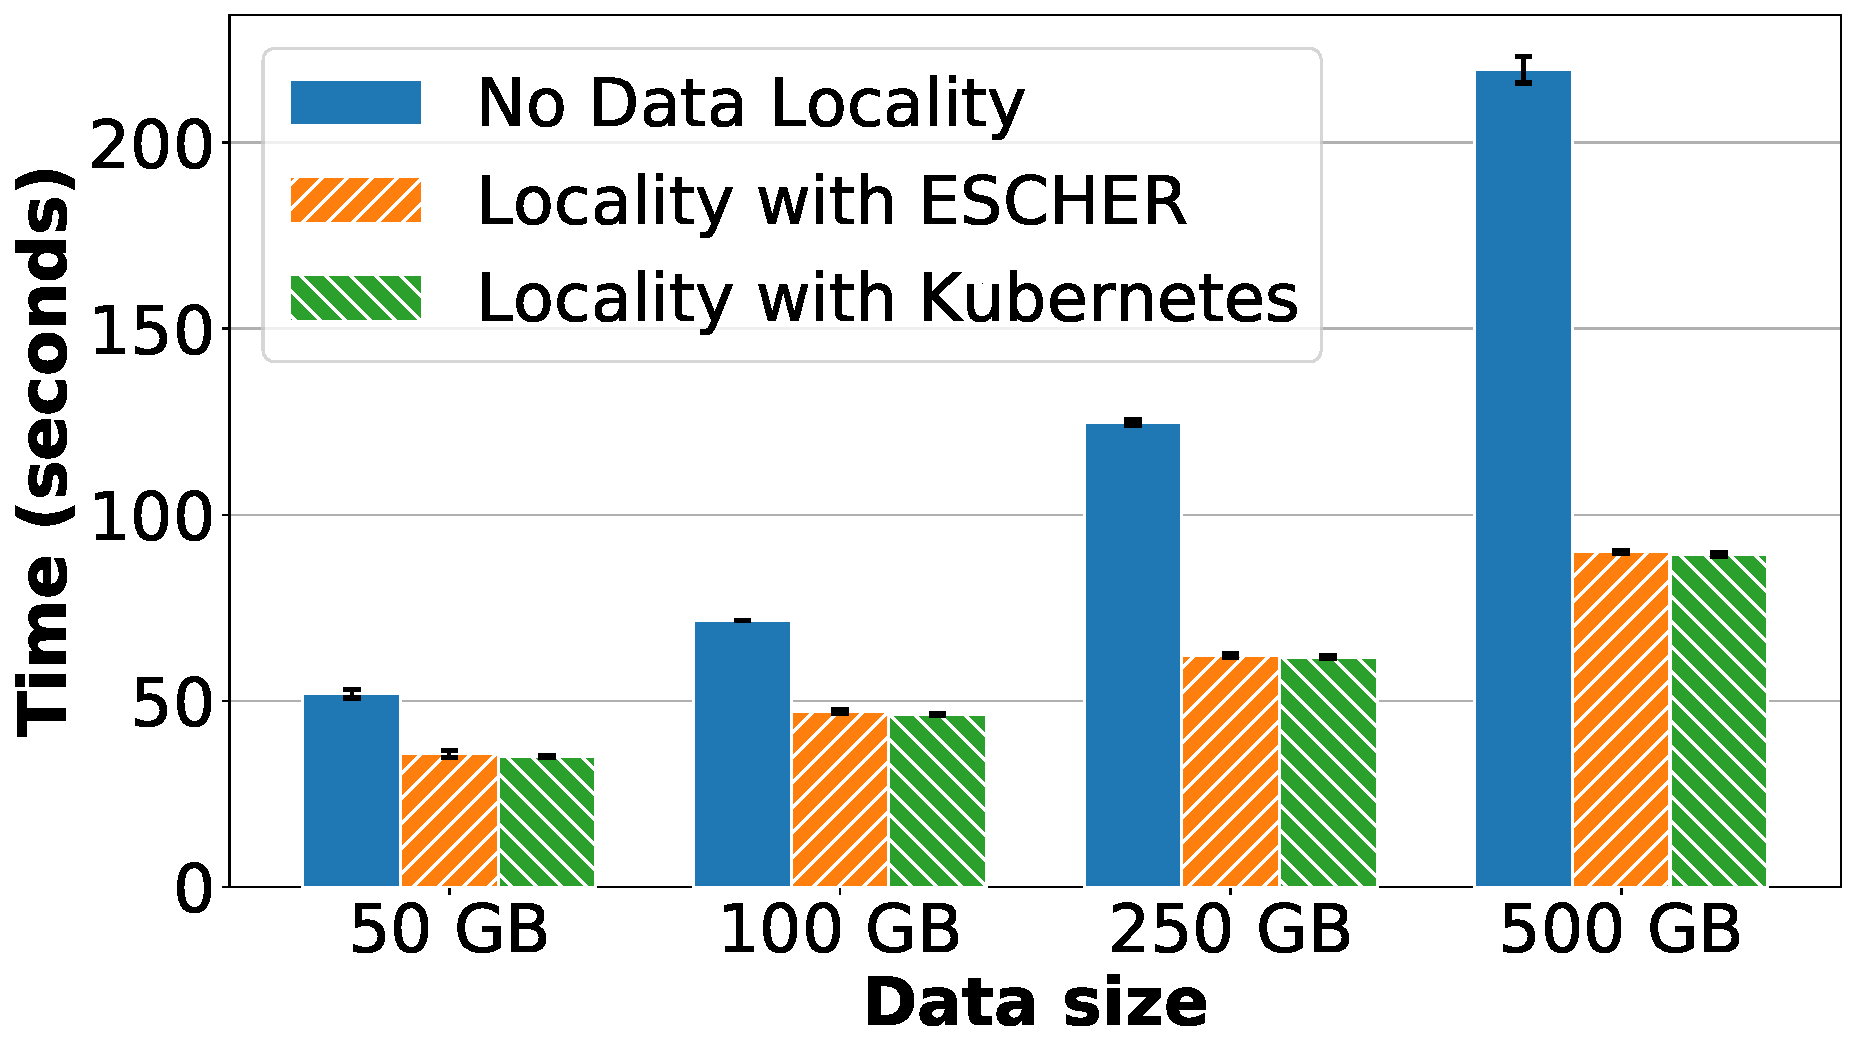
\includegraphics[width=0.8\columnwidth]{escher/plots/mapreduce_makespan.pdf}
% \caption{\small Makespan of WordCount running on a 100-node Kubernetes cluster, comparing a random placement policy, ESCHER on Kubernetes with data locality, and Kubernetes' native data locality.
% %A random placement policy has high network overheads due to poor data-locality. ESCHER implementation on Kubernetes performs comparably with the off-the-shelf core Kubernetes data locality policy.
% }
% \label{fig:mapreduce-makespan}
% \end{figure}

% \begin{table}[ht]
% \begin{center}
% \begin{tabular}{cccc}
% \toprule
% & \multicolumn{3}{c}{\textbf{Scheduler}}\\
% \textbf{Nodes}     & Generic & Kubernetes & ESCHER \\
% \midrule
% 10 & $183.32 \pm 0.51$ & $54.69 \pm 0.46$ & $55.24 \pm 0.39$ \\\hline
% 50 & $113.71 \pm 0.49$ & $44.02 \pm 0.27$ & $44.71 \pm 0.44$  \\\hline
% 100 & $51.90 \pm 0.31$ & $35.08 \pm 0.31$ & $35.76 \pm 0.49$  \\
% \bottomrule
% \end{tabular}
% \end{center}
% \caption{\small Makespan of WordCount MapReduce jobs in seconds, compared across varying cluster sizes.
% % As the cluster size increases, ESCHER scales similarly to core kubernetes scheduler, while outperforming the generic data-locality unaware scheduler.
% }
% \label{tab:mapreduce-xnode}
% %\vspace{-8mm}
% \end{table}


% \begin{figure}[ht]
% % \begin{subfigure}{1\linewidth}
% % \centering
% % 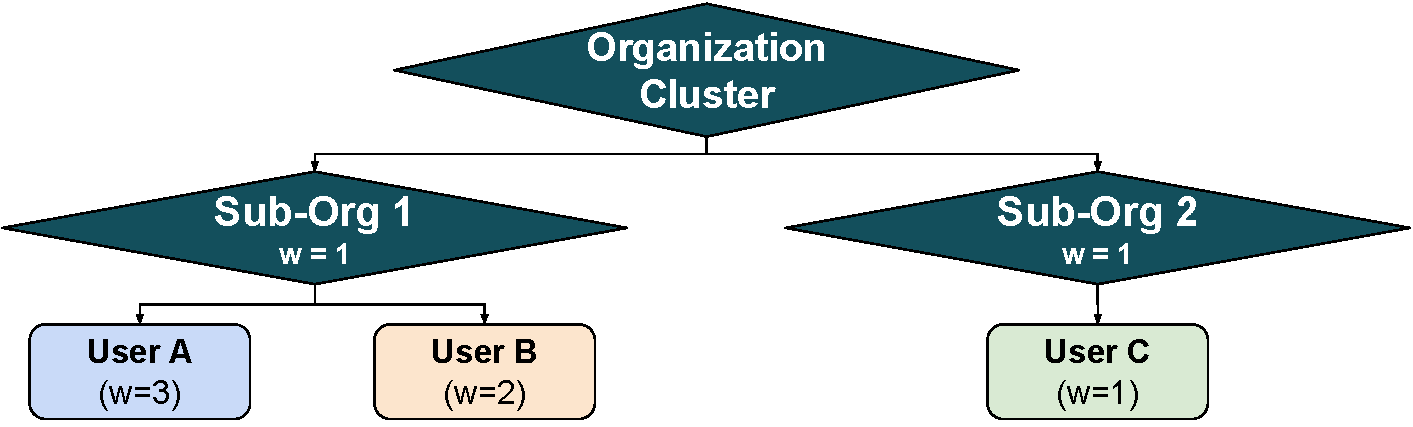
\includegraphics[width=1\columnwidth]{escher/plots/hfs/ESCHER_HFS_3User_OrgChart.pdf}
% % \caption{Organization Chart}
% % \label{fig:hfs-3user-orgchart}
% % \end{subfigure}
% % \begin{subfigure}{1\linewidth}
% \centering
% 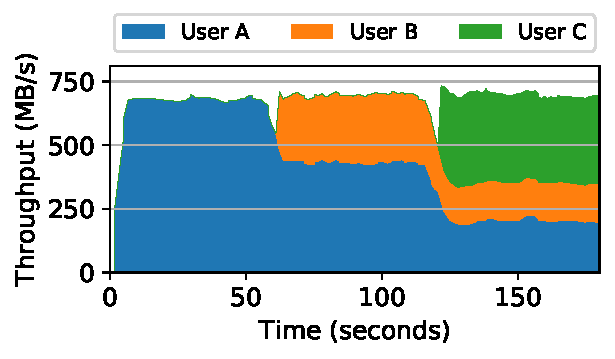
\includegraphics[width=0.93\columnwidth]{escher/plots/hfs/3user_hfs_sharing_mapreduce_50nodes_area_short.pdf}
% % \caption{User-wise throughput}
% % \end{subfigure}
% \caption{\small Per-user WordCount throughput with hierarchical max-min fair sharing.
% A and B are in Sub-Org1 with weights 2:3; C is in Sub-Org2.
% A, B, and C begin submitting tasks at $t=0,60,120$, respectively.
% %(a) shows the organization chart for resource sharing between sub-org 1 and sub-org 2. Weights (w) are relative to other users under the same parent.
% % (b) plots the throughput for users A, B and C on a cluster of 50 nodes.
% %At time t=0, only user A is submitting tasks so the HFS ESL allocates all resources to user A. At time t=60 and t=120, User B and User C start submitting tasks respectively.
% % The HFS ESLs adjust resource allocations based on utilization while maintaining organization level and sub-organization level weight proportional fairness.
% }
% \label{fig:hfs-3user-result}
% \end{figure}
% Two interfaces - infeasible and cancel tasks
% Throughput bug

% \begin{figure}
% \begin{subfigure}{1\linewidth}
% \centering
% 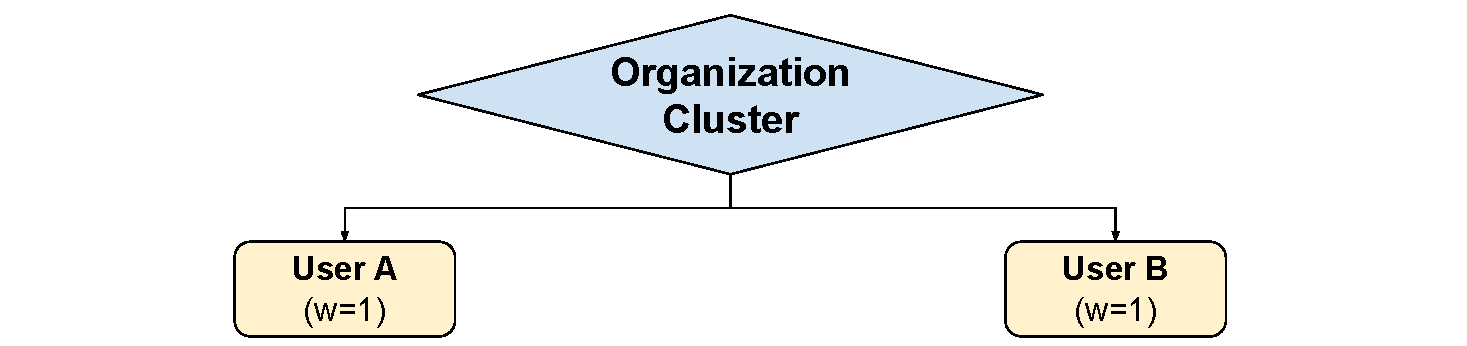
\includegraphics[width=1\columnwidth]{escher/plots/hfs/ESCHER_HFS_2User_OrgChart.pdf}
% \caption{Organization Chart}
% \label{fig:hfs-2user-orgchart}
% \end{subfigure}
% \begin{subfigure}{1\linewidth}
% \centering
% 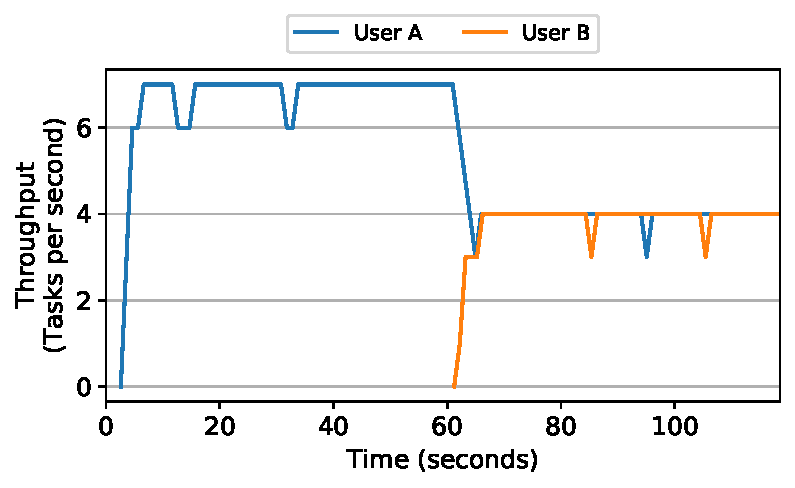
\includegraphics[width=0.9\columnwidth]{escher/plots/hfs/2user_hfs_sharing.pdf}
% \caption{User-wise throughput}
% \label{fig:hfs-2user-result}
% \end{subfigure}
% \caption{\small Min-Max Fair Sharing with ESCHER. Figure (a) shows the organization chart for resource sharing between User A and User B, each having equal weights (w=1). Figure (b) plots the throughput for users A and B. At time t=0, only user A is submitting tasks so the HFS ESL allocates all resources to user A. At time t=60 user B starts submitting tasks. The HFS ESL adjusts deallocates resources from user A and reassigns them to user B to maintain fairness.  
% }
% \label{fig:hfs-2user}
% \end{figure}

\subsubsection{Hierarchical max-min fair sharing}
\label{eval:hfs}
% Cool bits:
% \begin{itemize}
%     \item The resizing of the cluster is completely transparent to the users - they don't need to worry how many resources are allocated to them
%     \item Composition of data locality and fair sharing is as simple as adding resource requirements.
% \end{itemize}
Hierarchical Max-Min Fair Sharing (\Cref{policies}) allocates resources proportionate to a user's weight in a hierarchical organization.
% HFS maximizes resource utilization by reallocating idle resources.
Users submit jobs at different times, so their ideal absolute resource share is dynamic, making it impossible to maximize overall resource utilization with static labels.
% This makes it impossible to implement HFS with a static label-based scheduler since the resource share per user is dynamic.
For example, consider a two-team organization: Sub-Org1 with users A and B of weights 2:3, and Sub-Org2 with user C.
% with equal weights - Sub-Org1 and Sub-Org2. Sub-Org1 has two users, A and B with weights 2:3, while sub-org2 has one user C.
To ensure fairness with static labels, the only option is to allocate each user a fixed proportionate share, leading to under-utilization when only one user is submitting work.

% To achieve fairness, the only option with static labels would be to allocate each user a fixed share, leading to under-utilization in \Cref{fig:hfs-3user-result}. (i.e., A would only reach 200MB/s at $t$=0).

Because ephemeral resources can be \emph{dynamically} created and destroyed, an HFS policy ensures fairness while also maximizing overall utilization as users enter and leave the system~(\Cref{fig:hfs-3user-result}).
We deploy a HFS policy on a 100 node cluster running WordCount. We use a parent ESL for the teams and two children ESLs for Sub-Orgs 1 and 2 to create a hierarchy of ESLs.
An HFS ESL tracks idle resources and reallocates resources between teams or users.
% For example, at $t$=60 in \Cref{fig:hfs-3user-result}, B begins submitting tasks, causing the Sub-Org1 ESL to reclaim resources from A.
The workload in \Cref{fig:hfs-3user-result} starts with only user A submitting tasks to the scheduler. Since other users' resources are idle, the HFS ESLs re-allocate all idle resources to A to achieve max-min fairness. At time $t$=60, user B starts submitting tasks. This causes the Sub-Org 1 ESL to reclaim resources from A to re-allocate to B, in proportion to their weights. B's warmup time causes a small dip in net throughput at $t$=60. Finally at time $t$=120, user C starts submitting tasks and the parent ESL reallocates resources to Sub-Org2. Since Sub-Org 2 and Sub-Org 1 have equal weights, C's resource allocation is equal to the sum of A and B's allocation.
Ephemeral resources also enable composition: the application composes its custom policy (in this case, data locality for WordCount) with the two HFS ESLs by concatenating all the resource requirements.

% The workload in \Cref{fig:hfs-3user-result} starts with only user A submitting tasks to the scheduler. Since other users' resources are idle, the HFS ESLs re-allocate all idle resources to A to achieve max-min fairness. At time $t$=60, user B starts submitting tasks.
% This causes the Sub-Org 1 ESL to reclaim resources from A to re-allocate to B, in proportion to their weights. B's warmup time causes a small dip in net throughput at $t$=60. Finally at time $t$=120, user C starts submitting tasks and the parent ESL reallocates resources to Sub-Org2. Since Sub-Org 2 and Sub-Org 1 have equal weights, C's resource allocation is equal to the sum of A and B's allocation.

% Not only is ESCHER able to maintain the cluster's fair-sharing requirements, it also allows the each user to compose their application-level policies with cluster-level policies. This is achieved by simply concatenating the data-locality resources with the resource requirement vector from the fair-sharing ESL. This concatenation ensures that the scheduler places the tasks where both constraints - fairness and data-locality - can be satisfied.

% Using ephemeral resources also reduces implementation complexity by enabling transparent resizing of user shares when applying max-min fairness. Since the ESLs dynamically create and removes each user's ephemeral resources from underlying nodes, the users' applications are not required to keep a track of the resources allocated to them. This would not have been possible in a static label-based scheduler since the max-min shares for each user are dynamic. 



\subsubsection{AlphaZero}
AlphaZero \cite{silver2017mastering} is a reinforcement learning application for the board game Go.
%Unlike it's predecessor AlphaGo\cite{silver2016alphago}, AlphaZero does not require any human-generated training samples and can instead leverage reinforcement learning techniques to play and learn from games against itself.
%We base this experiment off an existing AlphaZero implementation \cite{anthony2017thinking}, which uses hard-coded process placement.
We demonstrate \name{}'s flexibility by porting an implementation~\cite{anthony2017thinking} onto Ray without compromising performance relative to the optimal hard-coded (but inflexible) placement.

AlphaZero executes a Monte Carlo Tree Search on the game state space in a CPU-intensive \textit{BoardAggregator} process. The search is guided by a \textit{PredictorAgent} running a neural network on a GPU which evaluates a board and predicts the associated reward.
%Based on this prediction, the \textit{BoardAggregator} generates new boards to explore and learn from.
% This pattern creates a tight feedback loop between the \textit{BoardAggregator} and the \textit{PredictorAgent}.
Co-locating \textit{BoardAggregator}s and their corresponding \textit{PredictorAgent}s on the same physical node is thus desirable to avoid network overheads from transferring board states. These pairings also require anti-affinity for load balancing and to avoid interference \cite{gandiva}.
%Many existing frameworks do not allow the expression of this composition of load-balancing and co-location policies, while others frameworks would require a tedious re-implementation of the scheduler. 
With ephemeral resources, this composed policy can be specified in 5 lines of code~(\cref{fig:alphazerocode}): we apply a load-balancing policy~(\Cref{tab:escher-constraints-policies}) to the \textit{PredictorAgent} and a co-location policy to the \textit{BoardAggregator} and \textit{PredictorAgent}.
%This composition takes only 5 lines of code (\cref{fig:alphazerocode}).

We ran 10k iterations of AlphaZero on a 32-node cluster (128 GPUs total). %board generation distributed across 16 machines with a total of 128 GPUs.
We compare three setups: 
(a) co-location with hard-coded placement,
(b) co-location with ephemeral resources, and 
(c) a baseline policy with no co-location. 
\Cref{fig:alphazerolatencycdf} plots the CDF for board exploration time. %, which includes generating the board on the \textit{BoardAggregator} and evaluating it on the \textit{PredictorAgent}. 
% Comparing the percentile distributions from this CDF in \cref{fig:alphazerolatencypxx}
Co-location is important for performance, outperforming no-colocation by 15.4\% in median latency and 20\% in P95 latency. %, demonstrating the benefits of co-location.
Additionally, co-location with ephemeral resources adds insignificant overheads of <1\%, while requiring less developer effort: the application code~(\Cref{fig:alphazerocode}) does not need to match \textit{PredictorAgent}-\textit{BoardAggregator} pairs to specific nodes.

% while providing a much simpler interface to express scheduling requirements.

%and by 714\% on P99.9 latency. P99.9 latency demonstrates the largest difference because the initial queries in the no-colocation case require setting up inter-machine communication sockets which may take time.

% Co-location with Logical Resources Stats - P999: 0.05949, P95: 0.02135, P50: 0.02083
% Static Co-location Stats - P999: 0.05863, P95: 0.02147, P50: 0.02079
% No Co-location Stats - P999: 0.06227, P95: 0.02578, P50: 0.02401


% \begin{figure}
% ~
% % Task co-location
% ~
% \begin{subfigure}{.22\textwidth}
%   \centering
%   \begin{minted}[fontsize=\tiny,breaksymbolleft=\tiny\ensuremath{},breakautoindent=true]{python}
% class PredictorAgent():
%   def __init__(id):
%     # Create resource for co-location
%     set_resource(label=id, capacity=1)
%     ...
%   \end{minted}
% \end{subfigure}
% ~
% % Task co-location
% ~
% \begin{subfigure}{.22\textwidth}
%   \centering
%   \begin{minted}[fontsize=\tiny,breaksymbolleft=\tiny\ensuremath{},breakautoindent=true]{python}
% class BoardAggregator():
%   def __init__(predictor):
%     # Assign predictor handle
%     self.predictor = predictor
%     ...
%   \end{minted}
% \end{subfigure}

% \newline

% \begin{subfigure}{.49\textwidth}
%   \centering
%   \begin{minted}[fontsize=\tiny,breaksymbolleft=\tiny\ensuremath{},breakautoindent=true]{python}
% def main():
%     # Create load-balancing resources
%     for node in cluster:
%         set_resource("load_bal", 1, node)
%     for i in range(0, num_agents):
%         p = PredictorAgent(resources = {"GPU": 1, "load_bal": 1}).launch(id=i)
%         # The predictor creates a resource with label i
%         # This resource is used by the BoardAggregator to co-locate.
%         b = BoardAggregator(resources = {i: 1}).launch(predictor=p)
%   \end{minted}
% \end{subfigure}
% \caption{AlphaZero placement preferences with \name{}}
% \label{figure:alphago}
% \end{figure}

\subsubsection{Distributed Training}
\label{sec:eval:tune}


% \begin{figure}
% 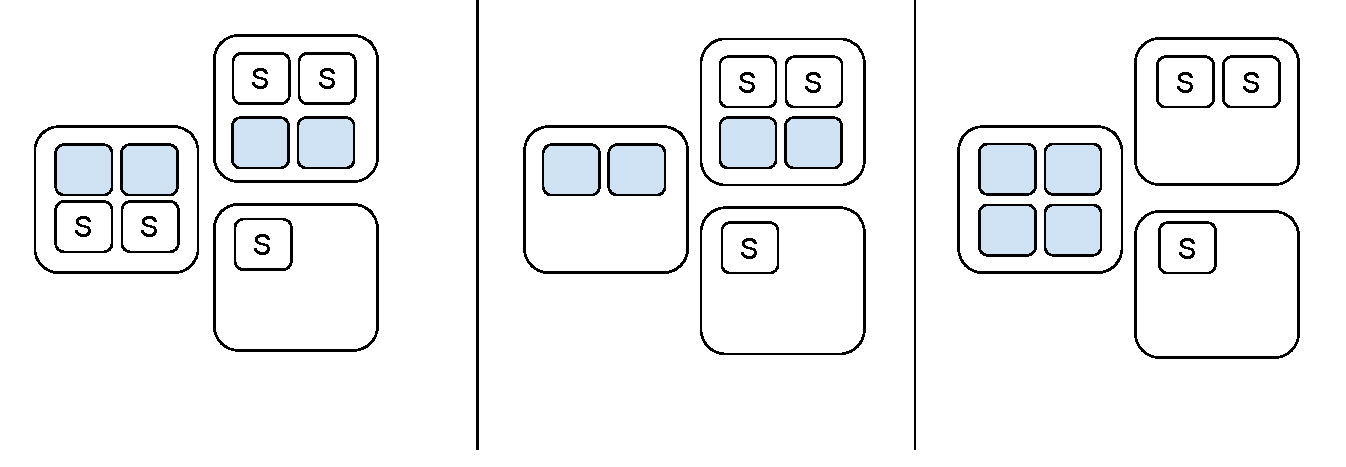
\includegraphics[width=0.9\columnwidth]{escher/figures/Eschertune.pdf}
% \caption{Migration after termination of the Short Job, signaling EscherTune to utilize a co-location mechanism and decrease communication overhead compared to Tune.
% }
% \label{fig:tune-results}
% \end{figure}



\def\longjob{\emph{long-job}}
\def\shortjobs{\emph{short-jobs}}
% Distributed training for a ML model typically consists of multiple workers that compute model updates in parallel and in lockstep.
For a distributed training job, worker placement is critical to performance, as co-locating workers reduces the cost of model synchronization at each step.
% The placement of these workers in a cluster is critical to the performance of the training process, as co-located workers avoid the network cost of model synchronization on each update operation.
%Typically, multiple jobs, each with different size and unpredictable completion time, will execute in parallel as part of a hyperparameter search~\cite{liaw2018tune}.
% Moreover, training jobs in a shared cluster can be of different sizes and with unpredictable completion times.
Gandiva \cite{gandiva} is a scheduler for deep learning jobs that aims to optimize training job performance. It composes a higher level \textit{load-balancing} policy and a lower-level \textit{co-location} policy to evenly spread jobs across machines while reducing intra-job communication overhead. 
To demonstrate \name{}'s flexibility, we augment Gandiva's \cite{gandiva} worker co-location and migration policy with Gang Scheduling to support distributed training jobs, and integrate the policy into Tune \cite{liaw2018tune}, an open source distributed training library built on Ray \cite{ray-osdi}, which we will refer to as \textit{EscherTune}.
We modified the Trial abstraction in Tune to be wrapped in a ghost task that ensures gang scheduling and applied co-location on tasks belonging to the same Trial.
%EscherTune records the current cluster placements during execution.
EscherTune triggers a migration whenever it detects sufficient available resources to place all workers of a job on the same node.
To execute a worker migration, EscherTune checkpoints the current job using application-specific checkpoint functionality and destroys all current workers. Then, EscherTune assigns ephemeral resources to the new target node, and relaunches all worker tasks of the training job without modifying their ephemeral resource requests.
 %To execute a worker migration, EscherTune will checkpoint the current training job using framework-dependent checkpoint functionality and destroy all current workers. Then, EscherTune assigns ephemeral resources to the target node and relaunches all worker processes of the training job with the specified ephemeral resource requests.
 
We compare EscherTune with Tune's open-source policy on a cluster of 12 GPUs. We launch 5 short-running training jobs (\shortjobs{}), each requiring 1 GPU, followed by 1 long-running training job requiring 4 GPUs (\longjob{}).
Each training job is training a ResNet-101 model on CIFAR-10 with a batch-size of 64 images per device.

Initially, the \shortjobs{} are load-balanced across the cluster, while the 4 workers of the \longjob{} are spread across the cluster depending on GPU availability. This is a sub-optimal placement, so EscherTune migrates the \longjob{} to colocate its tasks as soon as resources become available from a \emph{short-job} completion, resulting in 36.3\% higher throughput~(\Cref{fig:tune-results}).
Meanwhile, Tune uses a static placement, so the \longjob{}'s throughput remains the same.
% Figure \ref{fig:tune-results} compares throughput of \longjob{} in EscherTune and Tune, with all jobs launched at the same time. The throughput is low when the workers are spread across the cluster, but when there are sufficient resources to place workers on the same node, EscherTune is able to use ephemeral resources to migrate and co-locate all workers, increasing the throughput of the job by 36.3\%.
Furthermore, EscherTune's implementation consists of only 50 lines of Python, with no changes to Tune or the Ray scheduler. % a callback of 50 lines of Python, with \textit{no changes} to Tune.
 

% \begin{figure}[t]
% \centering
% 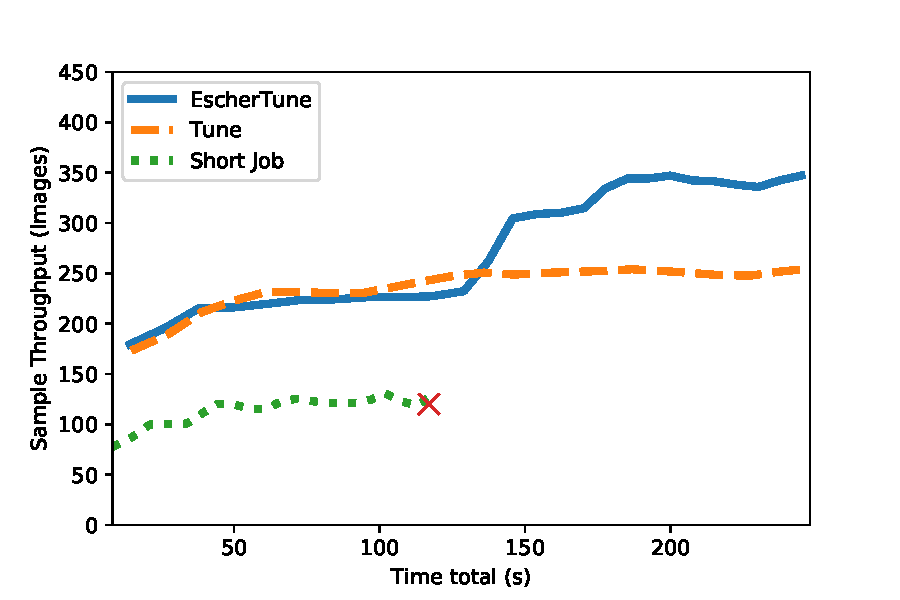
\includegraphics[width=0.85\columnwidth]{escher/plots/result_migrationthroughput.pdf}
% \caption{\small Throughput comparison of distributed training workloads with and without migration. ESCHER is able to augment an existing application, Tune, to increase sample throughput. 
% The red X indicates the termination of the short job, signaling EscherTune to utilize the co-location mechanism and decrease communication overhead compared to Tune.
% }
% % \caption{Throughput comparison of distributed training jobs with and without migration. 
% % Sample throughput for training can increase significantly by co-locating workers of
% % a distributed training job. In this mixed workload containing a distributed training job for a ResNet-101 architecture using 4 workers, ESCHER is able to easily augment the underlying framework to significantly improve performance. 
% % The red X indicates the termination of the Short Job, signaling EscherTune to utilize a co-location mechanism and decrease communication overhead compared to Tune.
% % }
% \label{fig:tune-results}
% \vspace{-0.3in}
% \end{figure}

% \subsubsection{Implementing Kube-Batch with ESCHER}
% To demonstrate ESCHER's ease-of-use, we add Gang Scheduling to Kubernetes using the Ephemeral Resources API and compare the implementation with a plug-in scheduler which adds this functionality to kubernetes. As described in Section \ref{sec:motivation}, adding gang scheduling to Kuberenetes in it's current form has been possible only through separate plug-in schedulers. One such plug-in is kube batch
\begin{figure*}[t]
\begin{subfigure}[b]{0.47\linewidth}
  \centering
\begin{subfigure}[t]{.22\textwidth}
  \centering
  \begin{minted}[fontsize=\tiny,breaksymbolleft=\tiny\ensuremath{},breakautoindent=true]{python}
class PredictorAgent():
  def __init__(id):
    # Create co-location resource.
    set_resource(
      name=id,
      capacity=1)
    ...
  \end{minted}
\end{subfigure}
~
% Task co-location
~
% \begin{subfigure}[b]{.21\textwidth}
%   \centering
%   \begin{minted}[fontsize=\tiny,breaksymbolleft=\tiny\ensuremath{},breakautoindent=true]{python}
% class BoardAggregator():
%   def __init__(predictor):
%     # Assign predictor handle
%     self.predictor = predictor
%     ...
%   \end{minted}
% \end{subfigure}
\begin{subfigure}[t]{0.72\textwidth}
  \centering
  \begin{minted}[fontsize=\tiny,breaksymbolleft=\tiny\ensuremath{},breakautoindent=true]{python}
def main():
  # Create load-balancing resources
  for node in cluster: set_resource("load_bal", 1, node)
  for i in range(0, num_agents):
    p = PredictorAgent(resources = {"GPU": 1, "load_bal": 1}).launch(id=i)
    # The predictor creates a resource with label i
    # This resource is used by the BoardAgg to co-locate.
    b = BoardAggregator(resources = {i: 1}).launch(p)
  \end{minted}
\end{subfigure}
  \caption{}
  \label{fig:alphazerocode}
\end{subfigure}
\begin{subfigure}[b]{0.26\textwidth}
  \centering
  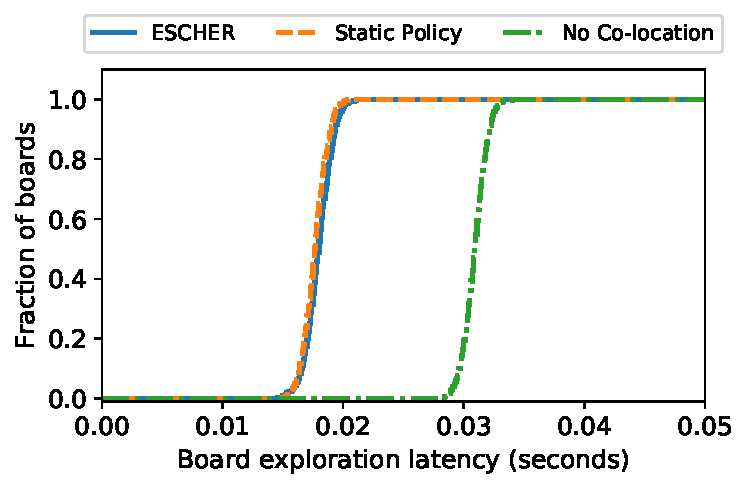
\includegraphics[width=\textwidth]{escher/plots/results_e2e_alphago_latencycdf_16node.pdf}
  \caption{}
  \label{fig:alphazerolatencycdf}
\end{subfigure}
\begin{subfigure}[b]{0.26\textwidth}
\centering
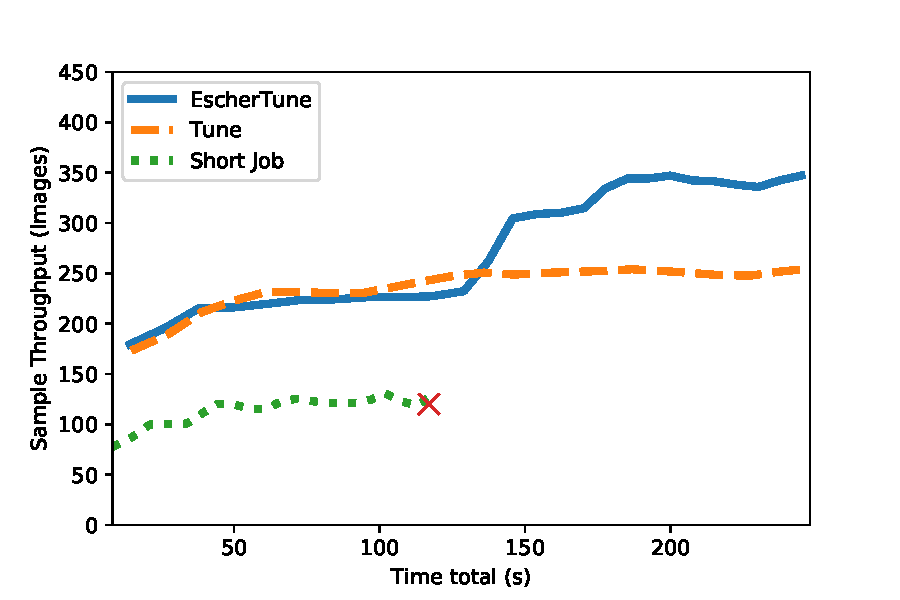
\includegraphics[width=\textwidth,trim=0cm 0cm 1.5cm 0cm, clip]{escher/plots/result_migrationthroughput.pdf}
\caption{}
\label{fig:tune-results}
\end{subfigure}
% \begin{subfigure}[b]{0.3\textwidth}
%   \centering
%   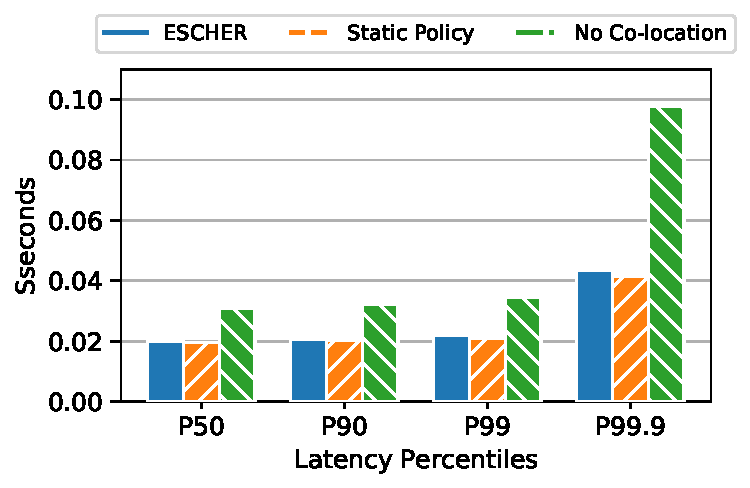
\includegraphics[width=\textwidth]{escher/plots/results_e2e_alphago_pxxcompare_16node.pdf}
%   \caption{}
%   \label{fig:alphazerolatencypxx}
% \end{subfigure}
\caption{\small AlphaZero and distributed training on \name{}. \textbf{(a)} Implementing AlphaZero policy with ESCHER, composing co-location with load-balancing.
% By co-locating the \textit{BoardAggregator}s and the \textit{PredictorAgent}s, the \name{} takes significantly lower time to generate and evaluate board states than an unaware scheduler. \name{} also performs comparably with a static policy that hard codes placement decisions, while offering the flexibility of a general scheduling policy.
\textbf{(b)} A CDF of AlphaZero board exploration latency, and
\textbf{(c)} Throughput comparison of a distributed training workload with a mix of short-running and long-running jobs. EscherTune is an augmentation of the hyperparameter search framework Tune~\cite{liaw2018tune}, using ESCHER to dynamically re-schedule jobs as others complete. %SCHER augments an existing application, Tune, to increase sample throughput. 
The red X indicates the completion of a short job. %, and EscherTune re-schedules the long-running job to claim the idle resources. % to utilize the co-location mechanism and decrease communication overhead compared to Tune.
}
\label{fig:alphazerolatencyfigure}
\vspace{-2mm}
\end{figure*}


\begin{figure}[t]
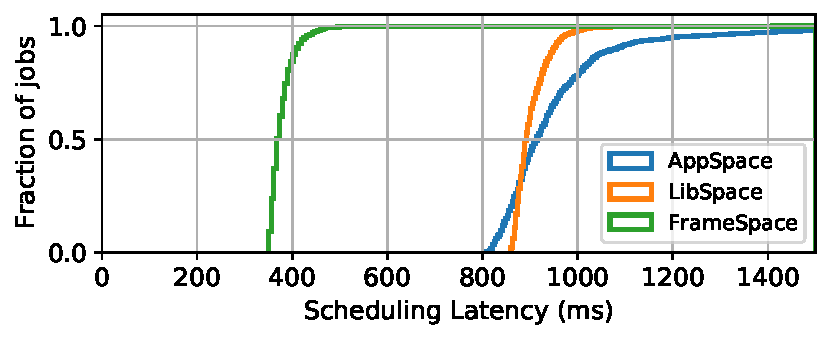
\includegraphics[width=0.92\columnwidth]{escher/plots/result_gangsched_design_compare.pdf}
\caption{\small Request latency for gang scheduling implemented in the application space, with (\textit{LibSpace}) and without (\textit{AppSpace}) coordination, versus the framework space (\textit{FrameSpace}). \textit{FrameSpace} is 1624 lines of code (LoC), \textit{LibSpace} with 261 LoC and \textit{AppSpace} with 78 LoC.}
\label{fig:gangscheddesign-results}
\end{figure}

\subsection{Microbenchmarks}
\subsubsection{Overhead of application-level policies}
\label{sec:eval:gangscheduling}
ESCHER scheduling policies can be implemented either in the application space for evolvability or in the framework for performance.
We evaluate the trade-offs involved in this choice by comparing three distinct designs of gang scheduling, all with ephemeral resources on Ray.

\textit{AppSpace} uses ghost tasks to atomically reserve resources (\Cref{policies:gangsched}).
% An application can call this policy without any coordination with another application in the same cluster.
While this policy is simple to integrate, the lack of coordination between applications can lead to deadlock, which must be resolved through timeouts. %it uses expensive ghost tasks to reserve resources and must resolve any livelocks through expensive timeouts.
\textit{LibSpace} avoids this by using a \emph{shared library}: a shared service in the cluster that serializes gang scheduling requests across applications.
% An application using \textit{LibSpace} sends all gang scheduling requests to this service, which returns the set of ephemeral resources that should be specified when submitting tasks.
\textit{LibSpace} thus avoids live lock entirely but requires deploying a separate shared service.
% \textit{LibSpace} improves upon this by using the same ghost task approach, but in a shared library which runs as a common service in the cluster to provide inter-job coordination. All jobs must communicate with this library to request gang scheduling of their tasks by specifying the resources required for scheduling all tasks. The library returns a ephemeral resource that must then be used by the application to place its tasks. \textit{LibSpace} is able to serialize gang scheduling across jobs, allowing it to avoid live-locks.
Finally, \textit{FrameSpace} modifies the Ray scheduler to expose a gang scheduling API.
Internally, a centralized service within Ray directly reserves and creates ephemeral resources.
Since it has direct access to the resource table, \textit{FrameSpace} avoids using ghost tasks, reducing overheads from worker allocation and task dispatch.

% implements gang scheduling as a part of the core Ray scheduler. This requires modifications in the core ray scheduler to expose an API for applications to request gang scheduling of their tasks. Internally, this implementation directly reserves resources in the scheduler's resource availability map and creates an ephemeral resource which is returned and requested by tasks to schedule their gang of tasks. 

\Cref{fig:gangscheddesign-results} compares the request latency of these designs on a 32-node cluster with 256 CPUs.
% We subsample 100k gang-scheduling requests from the Google ClusterData 2011 trace~\cite{clusterdata:Reiss2011}. % and measure the scheduling latency per request. %and measure the time taken from request submission to job start (scheduling latency).
% We subsample the Google ClusterData 2011 trace \cite{clusterdata:Reiss2011} to model request arrival patterns. 
% To evaluate the performance of these designs, we set up a cluster of 32 nodes with 8 CPUs each. We then submit 100k gang-scheduling requests over 15 minutes and measure the scheduling latency per request. %and measure the time taken from request submission to job start (scheduling latency).
% We subsample the Google ClusterData 2011 trace \cite{clusterdata:Reiss2011} to model request arrival patterns. Figure \ref{fig:gangscheddesign-results} compares the scheduling latency across the three designs.
While the mean latency of \textit{AppSpace} and \textit{LibSpace} is similar, \textit{AppSpace} has higher variance and a longer tail because it uses timeouts to break deadlocks.
\textit{LibSpace} incurs overhead from serializing requests at a separate service, resulting in a higher minimum latency. On average, \textit{FrameSpace} is nearly $2\times$ faster than \textit{AppSpace} and \textit{LibSpace} because it directly reserves resources instead of using ghost tasks. However, we note that for long-running tasks such as model training and batch processing workloads, the absolute scheduling latency is still a tiny fraction (<1s) compared to the runtime of the workloads (multiple hours). Moreover, implementing \textit{FrameSpace} is a significant effort, requiring a deep understanding of the Ray scheduler and modifying 1624 lines of Ray code.
To compare, \textit{LibSpace} and \textit{AppSpace} are implemented in 261 and 78 lines of \emph{application-level} code, respectively.



\subsubsection{Overheads of Ephemeral Resources}
% In this section, we evaluate the costs of introducing ephemeral resources in the framework scheduler.


%\textbf{Dynamic resource creation.}
%Scheduling with ephemeral resources relies on the ability to create and modify resources at run-time.
We evaluate the time to create resources and propagate their availability throughout the cluster.
Since the \lstinline{set_resource} call is asynchronous, we verify that the resources have been created and are available for use by launching no-op tasks that request these newly created resources. %The completion of these tasks marks the successful creation and propagation of ephemeral resources.
% \begin{figure}
%     \centering
%     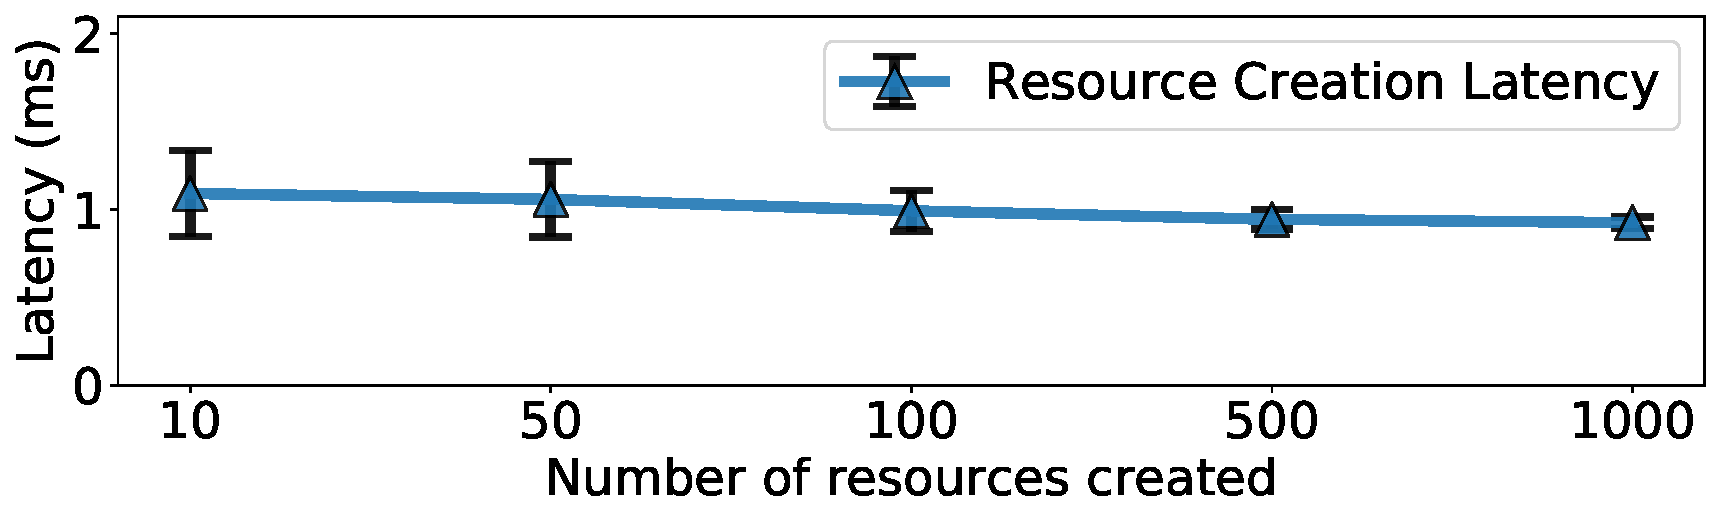
\includegraphics[width=\linewidth]{escher/plots/result_microbench_creationlatency_vs_numres.pdf}
%     \caption{\small Mean per-resource creation latency in Ray. Creating ephemeral resources in \name{} is a low cost operation that scales linearly with the number of resources created.}
%     \label{fig:res-creation-microbench}
% \end{figure}
Figure \ref{fig:res-creation-microbench} compares the mean latency of creating an equal number of resources on each node in a 50-node \ray{} cluster.
We show that even when creating 1000 ephemeral resources, we can maintain 1ms latency per request.
% against the number of resources created using the \lstinline{set_resource} API.
%Number of resources reflects the total resources created in the cluster, while the mean time to resource creation is measured as the time taken from the \lstinline{set_resource} submission to the availability of the resource.
As more resources are created, the cost of resource creation is amortized and the per-resource creation cost decreases to 0.72ms. 
In general, the overhead of creating or deleting an ephemeral resource should be roughly equivalent to that of a key-value store request.
% In absolute terms, the cost of creating ephemeral resources is insignificant, making \name{} a viable design.



\begin{figure*}[t]
\centering
\begin{subfigure}[b]{0.31\linewidth}
  \centering
  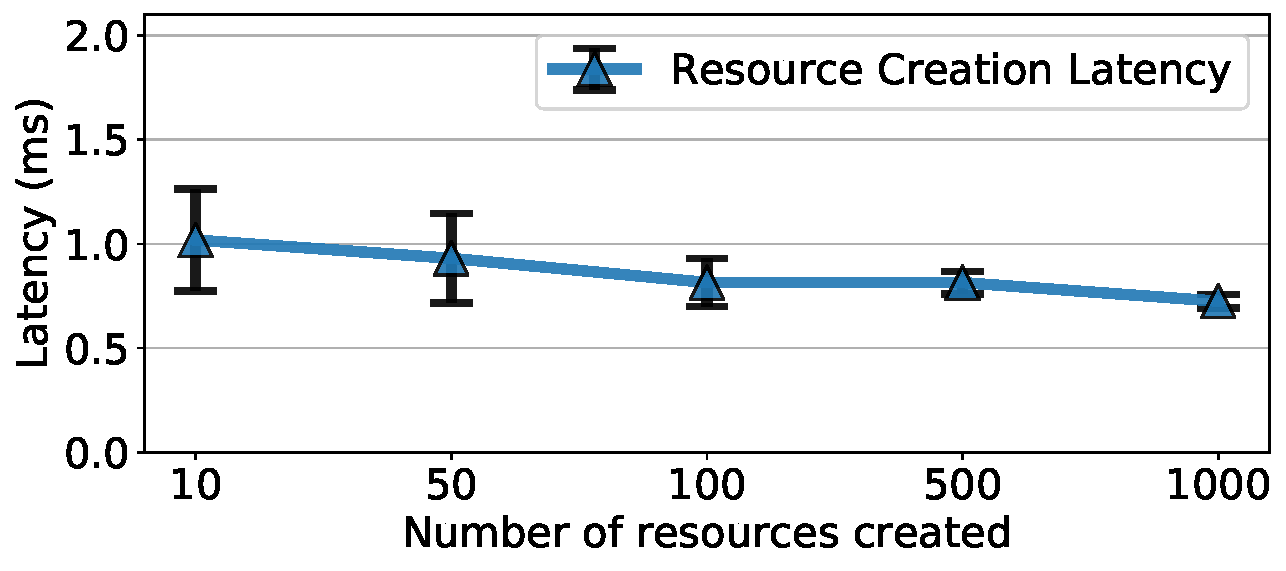
\includegraphics[width=\textwidth]{escher/plots/microbench_horz/result_microbench_creationlatency_vs_numres_horz.pdf}
  \caption{}
  \label{fig:res-creation-microbench}
\end{subfigure}
\begin{subfigure}[b]{0.31\textwidth}
  \centering
  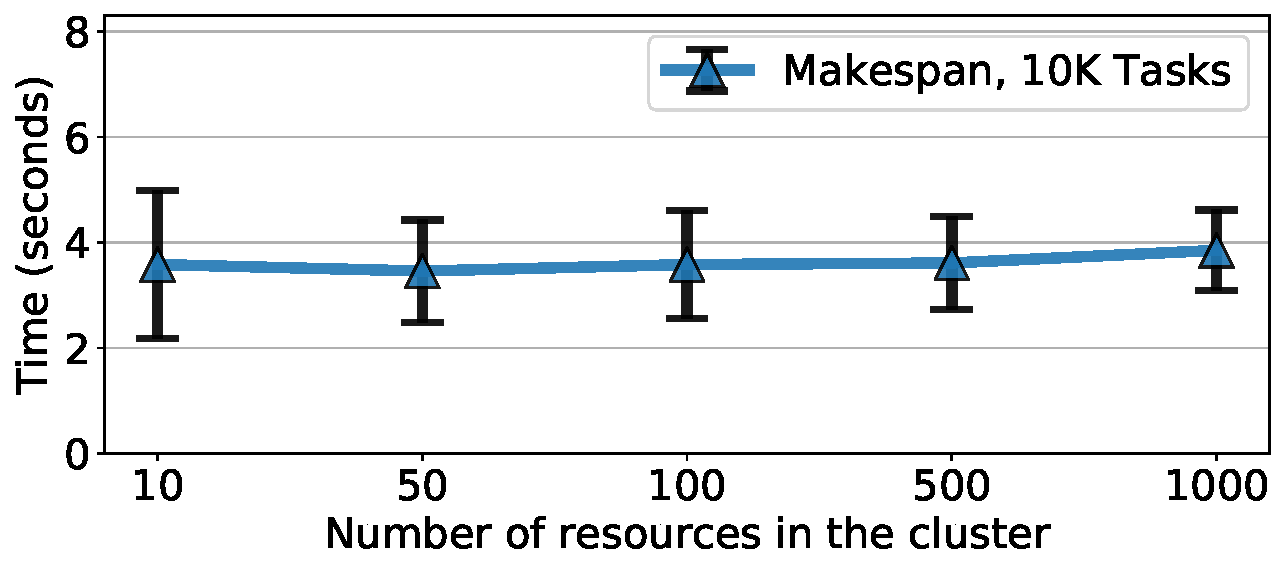
\includegraphics[width=\textwidth]{escher/plots/microbench_horz/result_microbench_schedlatency_vs_clusterresources_horz.pdf}
  \caption{}
  \label{fig:schedlatency-resources-microbench}
\end{subfigure}
\begin{subfigure}[b]{0.31\textwidth}
  \centering
  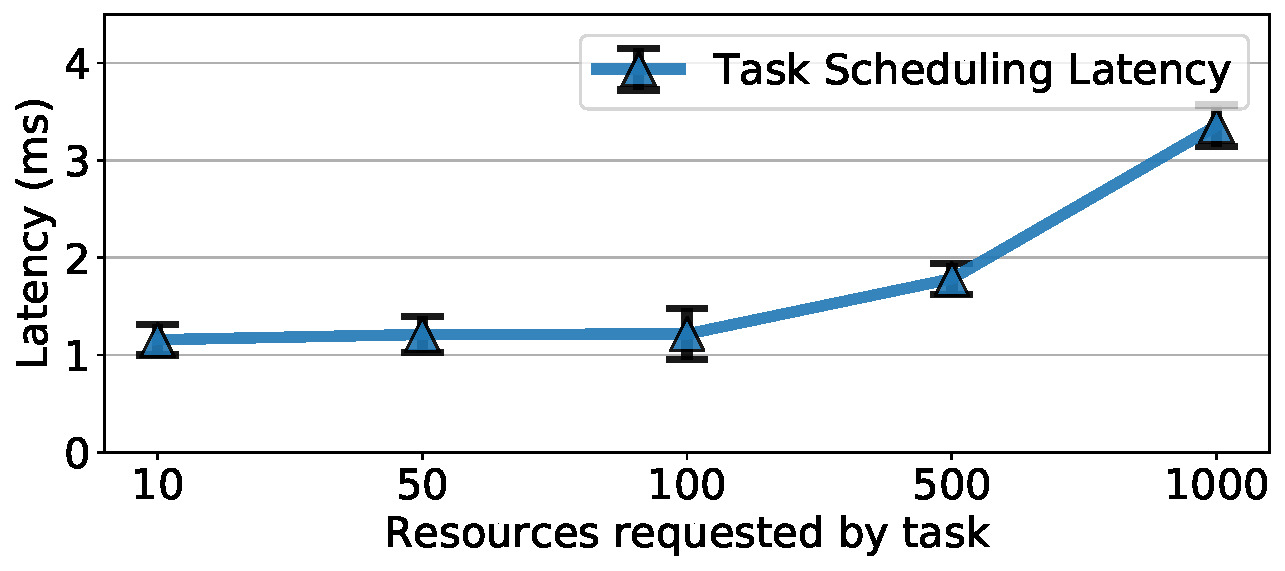
\includegraphics[width=\textwidth]{escher/plots/microbench_horz/result_microbench_schedlatency_vs_resrequested_horz.pdf}
  \caption{}
  \label{fig:schedlatency-taskrequest-microbench}
\end{subfigure}
\vspace{-4mm}
\caption{\small \name{} microbenchmarks. \textbf{(a)} Mean per-resource creation latency in Ray. Creating ephemeral resources in \name{} is a low-cost operation that scales linearly with the number of resources created. \textbf{(b)} Scheduling latency overheads from presence of ephemeral resources. Makespan of a 10000 task workload remains unaffected by the count of ephemeral resources in the cluster. \textbf{(c)} Effect of task resource requirements on scheduling latency in an environment with 10000 resources.}
\label{fig:microbenchfig}
\end{figure*}


\noindent\textbf{Ephemeral resources and scheduling latency.}
%The core task of the framework scheduler is to match task resource requirements with cluster resource availability.
The creation of ephemeral resources may add burden to the scheduler, as it must consider a greater number of attributes during resource matching.
% The usage of ephemeral resources imposes an additional burden on the scheduler and its resource matching complexity, as the number of resource attributes managed by the scheduler and the dimensionality of compared resource attribute vectors grows. 
Therefore, we analyze the effect of resource creation on task scheduling latency. We create an equal number of resources across 50 \ray{} nodes in a cluster using the \lstinline{set_resource} API. We then evaluate two cases based on the resource requirements of the tasks involved.

% \textbf{Tasks without resource requirements.}
First, in Figure~\ref{fig:schedlatency-resources-microbench}, we launch 10,000 tasks, none of which require any ephemeral resources to be scheduled. %, and measure the makespan of this workload against the number of resources present in the cluster.
As the tasks do not have any specific resource requirements, the scheduler execution time and workload makespan are not affected by the number of ephemeral resources present. %, and the makespan of the workload remains unaffected even by the presence of other ephemeral resources in the cluster.

% we highlight the effects of presence of ephemeral resources on scheduling latency for tasks that do not make use of ephemeral resources. In this microbenchmark, we launch a workload of 10k tasks, none of which require any ephemeral resources to be scheduled and compare the makespan of this workload against the number of resources present in the cluster. As the tasks do not have any specific resource requirements, the scheduler execution time remains constant, and the makespan of the workload remains unaffected even by the presence of other ephemeral resources in the cluster.
        % \begin{figure}
        %     \centering
        %     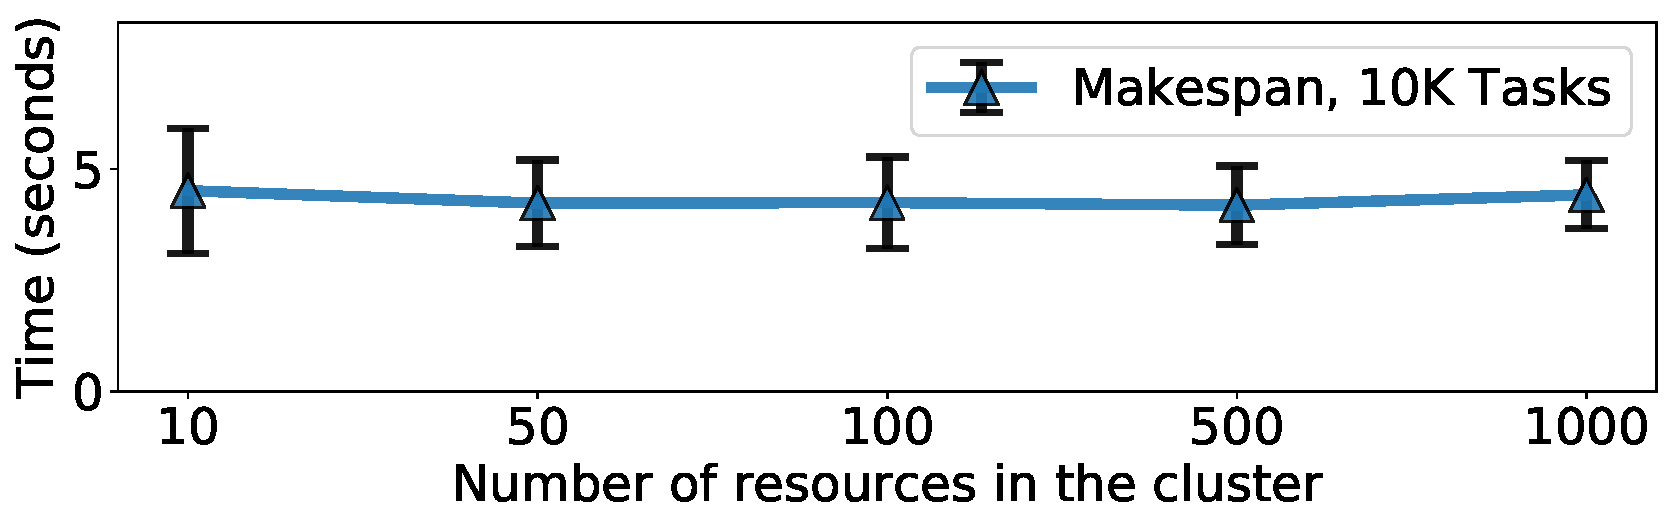
\includegraphics[width=\linewidth]{escher/plots/result_microbench_schedlatency_vs_clusterresources.pdf}
        %     \caption{\small Scheduling latency overheads from presence of ephemeral resources.  The makespan of a  10000 task workload remains unaffected by the count of ephemeral resources present in the cluster. }
        %     \label{fig:schedlatency-resources-microbench}
        %     \vspace{-4mm}
        % \end{figure}
        
% \textbf{Tasks with resource requirements.}
Second, when tasks do request ephemeral resources, the core scheduler must match the task's requirements to a set of candidate nodes.
To evaluate the overheads introduced by this matching, we setup a 50 node \ray{} cluster and create 1000 unique ephemeral resources evenly spread across nodes.
Figure 8c highlights the scalability of the scheduler as the number of ephemeral resources requested by a task grows. The the task scheduling latency grows only from 1.1ms to 1.2ms when requesting 1 vs. 100 ephemeral resources, respectively. We note that all policies described in this work require only a few ephemeral resources to express.
% We then perform multiple trials that launch a no-op task that requests a range from 10 to 1000 distinct resources.
%Figure \ref{fig:schedlatency-taskrequest-microbench} shows the scheduling latency of a no-op task against the number of resource requested by the task. The scheduling latency remains constant up to requests as large as 100 resources. Note that even the most complex scheduling policies do not require more than a few ephemeral resources.
    
        % \begin{figure}
        %     \centering
        %     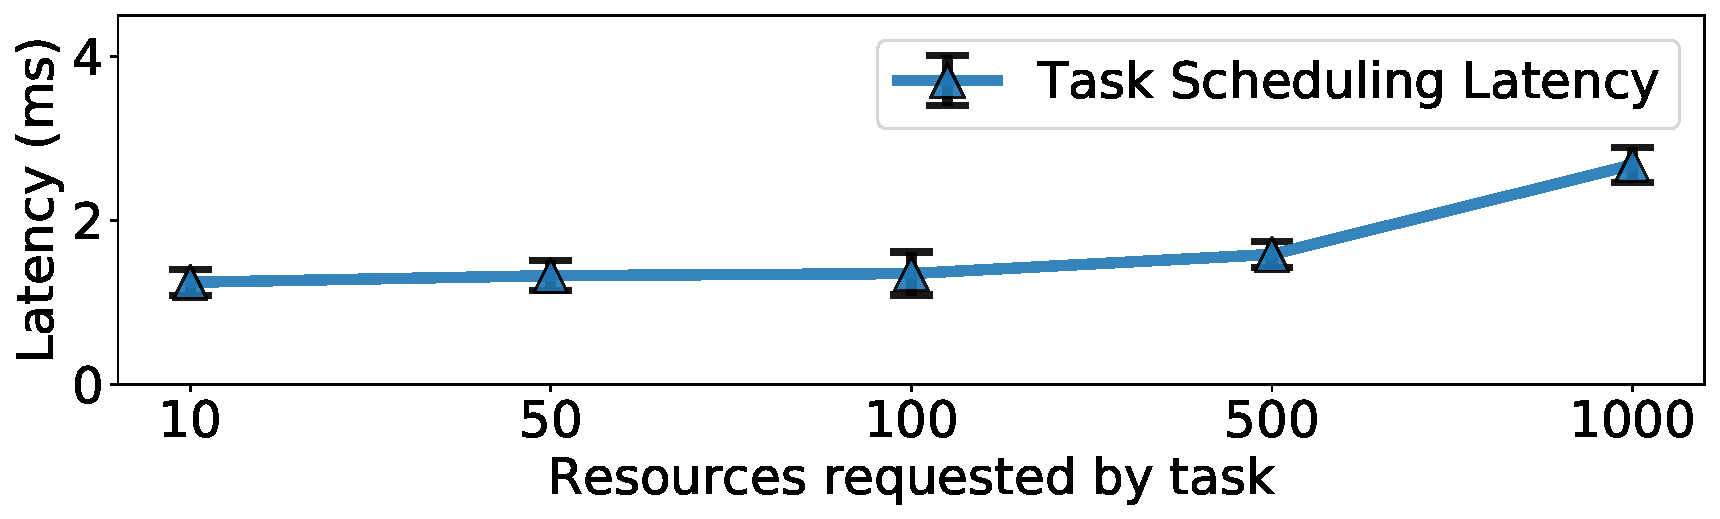
\includegraphics[width=\linewidth]{escher/plots/result_microbench_schedlatency_vs_resrequested.pdf}
        %     \caption{\small Effect of task resource requirements on scheduling latency in an environment with 10000 resources spread over 10 nodes. As a task resource requests more resources, the scheduling latency increases, but even the most complex scheduling policies do not require more than tens of resources. }
        %     \label{fig:schedlatency-taskrequest-microbench}
        % \end{figure}


% \textbf{Value of Locality-Aware scheduling.} In this microbenchmark, we study the motivation for co-location of tasks with the data they operate on. Specifically, we aim to evaluate the network cost of placing tasks and data on separate physical machines. We create arrays of varying sizes across 2 nodes in a \ray{} cluster and run two sets of tasks which fetch the data and perform a no-op. The first set of tasks uses ephemeral resources to co-locate with the data each task works on, while the other set of tasks is randomly placed.

% Figure \ref{fig:locality-latency} compares the task latency when tasks are co-located against random placement. \textcolor{red}{These numbers will be more dramatic soon - this run is local on one machine. Also, Is this a useful microbenchmark?}.

%     \begin{figure}
%         \centering
%         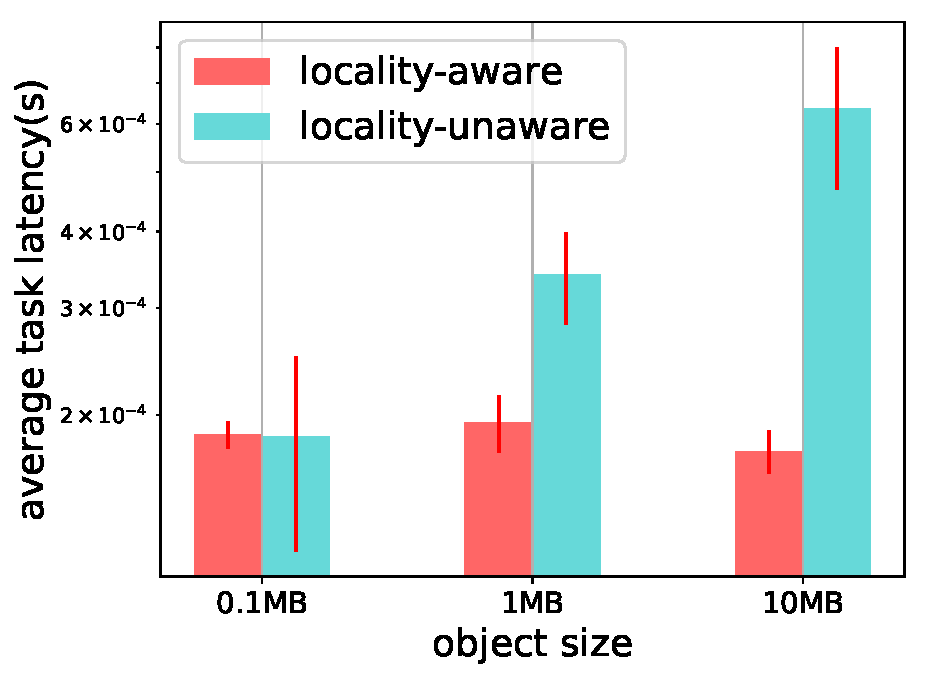
\includegraphics[width=\linewidth]{locality-latency.pdf}
%         \caption{Task-latency - Data-locality vs object size.}
%         \label{fig:locality-latency}
%     \end{figure}

% \subsection{Discussion}
% \textbf{Performance-evolvability tradeoff.} As we implemented our evaluation workloads, we found that \name{} significantly reduced the effort to express the workloads' scheduling constraints. In the AlphaZero workload, it required only 5 lines of code to be changed to express a composition of load-balancing and co-location. Implementing the same policy in Ray would have required re-writing the scheduler to enforce this policy on all tasks, since there is no policy selection mechanism in Ray. Same was true for implementing Gang Scheduling.

% However, as we see in the Gang Scheduling microbenchmark, the ghost task mechanism introduces latency due to the back-off performed by each ghost task on failure. While this latency is insignificant for long-running tasks, such as in distributed training, we acknowledge that this is a natural tradeoff ESCHER makes. It sacrifices performance for certain policies in favor of significantly reducing the implementation burden at the application-level. This gain in evolvability can be valuable for many applications, for whom functionality in the short-term (while the policy is integrated into the scheduler) may be more important than performance. 

% \textbf{Debugging ESCHER policies.} Since ephemeral resources are declarative in nature, debugging them requires replay of resource creation/deletion logs, which can be challenging.

\section{Discussion}
\label{discussion}

\noindent\textbf{Why use ESCHER?}
%For common scheduling policies, ESCHER's primary benefit compared to a monolithic cluster manager is not performance.
%Rather, its benefit is making it easy for an application to specify and implement unsupported policies without requiring any changes to the cluster scheduler. This is essential for developing new applications with sophisticated scheduling constraints that are not yet supported by the underlying scheduler.
For common scheduling policies, ESCHER’s primary benefit compared to a monolithic cluster manager is not performance. Rather, it's the ease to specify and implement new policies without requiring any changes to the cluster scheduler. This unlocks developing new applications with sophisticated scheduling constraints that are not yet supported by the underlying scheduler.
One example is the \emph{composition} of affinity and gang scheduling policies used in the distributed training example in \Cref{sec:eval:tune}, which is not supported by Ray's native scheduling primitives. Another example is DAG-based scheduling, which is offered natively by Ray but not Kubernetes.
DAG-based scheduling can be implemented by leveraging the task signaling primitive~(\Cref{sec:sched:primitive}). Effectively, ESCHER expands the set of policies a monolithic cluster manager can support.

%  For instance, the composition of affinity and gang scheduling policies in the EscherTune application was trivially achieved by concatenating gang scheduling and affinity ephemeral resource requirements. Implementing the same policy without ESCHER is possible, but would have required a deep understanding of the ray scheduler source code and would be a significantly larger effort to develop a new scheduling API. Similarly, DAG scheduling can expressed in ESCHER as a simple composition of the Task Signaling primitive defined in Section \ref{sec:sched:primitive}. Applying DAG scheduling otherwise requires integrating a completely different system, such as Apache Airflow\cite{airflow}.

Two-level schedulers~\cite{omega, mesos} achieve the same goal by exporting scheduling control directly to applications, but in doing so they also require applications to implement the entire scheduler themselves~(Section \ref{sec:arch:evolve}). ESCHER on the other hand requires minimal changes to application code: it required adding only two lines of code to MapReduce, five lines to AlphaZero and fifty lines to EscherTune, each of which had widely varying policy requirements. For policy composition especially, this ease of development is due in part to the use of ESLs.

% While the performance of ESCHER is often comparable to a hardcoded policy in the cluster scheduler, the primary value-add of ESCHER is that is allows the application to specify a policy without requiring any changes to the underlying framework scheduler. We note that two-level schedulers \cite{omega, mesos} also achieve the same goal by exporting scheduling control directly to applications, but in doing so they also require applications to implement a scheduler which must reason about tasks and resources in a distributed environment (Section \ref{sec:arch:evolve}). ESCHER on the other hand requires minimal changes to application code - it required adding only two lines of code to MapReduce, five lines to AlphaZero and fifty lines to EscherTune, each of which had widely varying policy requirements. 

% Additionally, some policies are very naturally expressed in ESCHER. For instance, the composition of affinity and gang scheduling policies in the EscherTune application was trivially achieved by concatenating gang scheduling and affinity ephemeral resource requirements. Implementing the same policy without ESCHER is possible, but would have required a deep understanding of the ray scheduler source code and would be a significantly larger effort to develop a new scheduling API. Similarly, DAG scheduling can expressed in ESCHER as a simple composition of the Task Signaling primitive defined in Section \ref{sec:sched:primitive}. Applying DAG scheduling otherwise requires integrating a completely different system, such as Apache Airflow\cite{airflow}.

% ESCHER on the other hand requires applications to only specify the policy as ephemeral resource requirements which requires minimal changes to existing code - it required adding only two lines of code to MapReduce, five lines to AlphaZero and fifty lines to EscherTune, each of which had widely varying policy requirements. 
%\noindent\textbf{Limitations and future work.} 
\noindent\textbf{Limitations.} 
A key goal of ephemeral resources is to provide a simple and narrow API that is easy to implement by most cluster managers. As a result, ESCHER eschews abstractions that would require complex implementations such as transaction support~\cite{omega} (which would allow to trivially implement gang scheduling) or utilization-based scheduling, such as load balancing~(\Cref{sec:softconstraints}).     
%This decision  Thus, ESCHER does not allow transactions on resource availability, such as for gang scheduling or resource utilization-based policies~(\Cref{sec:softconstraints}). 
While the application can still implement these policies using ghost tasks, these implementations have inherently a higher overhead. 
%This affects performance, as developers need to implement such functionality at the application level which is inherently slower and sometimes more cumbersome. 
%when compared to implementing the policy in the scheduler or providing transaction semantics to applications like Omega\cite{omega} does.
% Only after submitting a task can an application know if sufficient resources are available to execute the task.
%However, as we show in \Cref{sec:eval:gangscheduling}, the application can still use ghost tasks to implement such scheduling policies with relatively low overhead.
Of course, if applications require higher scheduling performance, we can eventually implement these policies in the cluster manager. Even in this case, ESCHER remains valuable as it can bridge the gap by enabling the applications to implement these policies before the cluster manager does.

%Meanwhile, the framework developer is still free to eventually integrate such policies into the core scheduler, e.g., when user demand for high performance increases, alongside the ephemeral resources abstraction.

Another limitation of ESCHER is that it doesn't expose the resource availability to the application, which means that the only way for an application to learn that there are not enough resources available is by submitting a task which hangs. As a result, the application might have to explicitly kill the tasks that hang, adding to the complexity. We do not expose resource availability is because it would not fully solve the problem: there is still a race condition when two tasks on different machines simultaneously request more than the available resources (e.g., a single GPU is available and two tasks simultaneously request one GPU each). This problem is exacerbated by the fact that ephemeral resources can be dynamically created, modified, or destroyed. One solution to this problem is providing transaction semantics, which, as mentioned above, ESCHER eschews due to its complex implementation. An avenue for future work would be to alleviate the challenges of handling such a dynamic environment, e.g., by using lazy execution or extending the API to allow constraints on ephemeral resources.

%Another fundamental property of ESCHER is that ephemeral resources are created, destroyed, and requested dynamically. Only after submitting a task can an application know if sufficient resources are available to execute the task, and even then the required resources may be created or destroyed asynchronously.
%Analogous to the differences between interpreted and compiled languages, the dynamic nature of ESCHER grants high development velocity by supporting a wide range of policies.
%However, since the result of the API calls depends on run-time information, it can also be more difficult to prove correctness and debug.
%Future work could explore ways to guarantee correctness in this completely dynamic setting, e.g., through lazy execution or by placing constraints on the ephemeral resources API.

%  This dynamic nature grants ESCHER its flexibility in supporting a wide range of policies. However, since the result of the API calls is dependent on the state of the cluster, it can be non-trivial to prove correctness of policies implemented in ESCHER. In contrast, schedulers using a declarative language for policy specification (SQL in DCM \cite{dcm-osdi20}, STRL in Tetrisched\cite{tetrisched}) can employ static checking to verify correctness of policies. Future work can explore how a static policy plan can be generated from a dynamic specification in ESCHER for verifying correctness. \romil{We need better future work here}

% A fundamental difference between ESCHER and other schedulers is that applications in ESCHER cannot perform transactions on resource availability, such as for placing reservations.
% Only after submitting a task can an application know if sufficient resources are available to execute the task. An ESCHER application must use mechanisms such as ghost tasks to perform incremental locking on resources, such as for gang scheduling. It also complicates (but does not preclude) the implementation of resource utilization based policies, such as the objective functions in \cref{sec:softconstraints}.

% Not providing transactions on resources is a deliberate design choice made in ESCHER. First, scheduling logic in an application gets significantly more complex if it must operate under transaction semantics. For instance, applications running on Mesos\cite{mesos} need to implement a local resource manager for book keeping of the offered resources and the tasks they are assigned to. Second, we discover that ghost tasks in ESCHER achieve the same goal through incremental locking without requiring any concurrency control support from the framework scheduler, such as in Omega\cite{omega}. As shown in \cref{sec:eval:gangscheduling}, ghost tasks introduce an overhead but significantly reduce the implementation complexity of both the application and the scheduler. This is also an opportunity for future work, where the framework can offer a dynamic choice between transactions for performance-sensitive applications, while allowing ghost tasks for developer agility.
%\swang{Not sure if I understand what "hybrid of transactions" means?}


% Can also start like - ESCHER's flexibility stems from its dynamic nature..  or, Unlike other static 
% Another fundamental property of ESCHER is that policies are defined and executed dynamically. Policy specification is done by invoking the \lstinline{set_resource} API at runtime and the policy is executed by requesting ephemeral resources at task submission. This dynamic nature grants ESCHER its flexibility in supporting a wide range of policies. However, since the result of the API calls is dependent on the state of the cluster, it can be non-trivial to prove correctness of policies implemented in ESCHER. In contrast, schedulers using a declarative language for policy specification (SQL in DCM \cite{dcm-osdi20}, STRL in Tetrisched\cite{tetrisched}) can employ static checking to verify correctness of policies. Future work can explore how a static policy plan can be generated from a dynamic specification in ESCHER for verifying correctness. \romil{We need better future work here}

% \swang{I like the above points about ghost tasks (as long as we're not duplicating them elsewhere, but it'd be good to mention at least one other limitation. Otherwise it will come off as not very enlightening for a discussion section.}


\section{Related Work}
\label{sec:related-work}



%Cluster scheduling has received considerable attention over the past few decades. Unfortunately, despite this attention, most schedulers are not general enough to simultaneously support or compose the variety of policies required by increasingly complex distributed applications.
%Here, we discuss some of the most representative cluster schedulers proposed so far \rliaw{better intro herre}.

%Most schedulers are not general enough to simultaneously support or compose the variety of policies required by increasingly complex distributed applications.

\textbf{Monolithic schedulers.}
Monolithic cluster schedulers aim to implement both the scheduling policy and mechanism for a distributed application.
Some provide a single generic scheduling discipline, such as fair sharing~\cite{isardquincy,ghodsi2011dominant}, gang scheduling~\cite{mpi}, or delay scheduling~\cite{delay-scheduling}. These schedulers provide little control to the application beyond the ability to set some configuration knobs, such as the time to wait before scheduling a task on a node that doesn't store its inputs~\cite{delay-scheduling}.
%Because these schedulers target a specific policy, they are inflexible and support only a limited set of applications.

Other monolithic schedulers aim for generality and provide APIs to allow applications to express scheduling constraints.
Examples are YARN~\cite{yarn}, Condor's ClassAds~\cite{condor}, and Kubernetes~\cite{kubernetes}.
Their monolithic design makes it hard to add support for new policies and their compositions.
For instance, adding support for gang scheduling to Kubernetes requires deep structural and API changes, and was eventually implemented as a standalone system~\cite{kubernetes-gang-scheduling}.
Often the API they provide is complex as well, since it must be expressive enough to capture complex constraints such as composition. 
For instance, the specification of ClassAds~\cite{classads} is 35 pages~\cite{classads-refman}.
\name{} achieves both \textit{simplicity} and \textit{evolvability} by decoupling policy specification and the resource-matching mechanism.
% This abstraction is backed by a basic scheduler that implements only one functionality: ensure that the capacity constraints of all resources are satisfied.
% This results in a simple design that is easy to scale and enables expression of dynamic and composable policies that cannot be supported in monolithic schedulers.

Like ESCHER, DCM~\cite{dcm-osdi20} also aims to maximize extensibility of framework schedulers by using a declarative model for applications to specify their desired policy behavior as SQL queries. In doing so, DCM deploys a custom scheduler and optimizer running with Kubernetes.
%These queries operate on cluster state stored in a database and are encoded as optimization problems to be solved by off-the-shelf solvers.
While this is well suited for policies which optimize for global objectives, expressing application-level constraints requires users to create and maintain a table in cluster state database, which can be challenging in a distributed environment. ESCHER's emphasis lies on supporting application-level scheduling goals, allowing it to easily handle task-task dependencies (Primitive P2 in \cref{sec:sched:primitive}). Moreover, \name{} reuses existing virtual resource implementations, thus requiring no additional services or schedulers to be deployed in the cluster framework.

Rayon~\cite{rayon} is a space-time reservation admission system, allowing applications to reserve a \textit{skyline} of resource capacity, $c(t)$, as a function of time. ESCHER can implement a discrete version of this by having a ghost task evaluate $c(t)$ and update ephemeral resources to match $c(t)$ at any instant.

\noindent\textbf{Two-level schedulers.}
% At the other extreme, there are schedulers which give all resource management and scheduling control to applications.
Rather than trying to implement application level policies, some cluster management frameworks are designed explicitly to give all resource management and scheduling control to the application.
Many of these frameworks employ a two-level hierarchy~\cite{yarn,mesos}, where the first level manages only resource isolation between applications, while the second level exposes physical resources to applications. These applications are then responsible for building their own scheduler. Omega~\cite{omega} follows a similar separation by providing transaction semantics on a shared cluster state for distributed schedulers.
While this approach grants maximum flexibility to applications, it adds significant complexity to application code since the application must now handle both scheduling policy and the mechanisms to ensure resource coordination between tasks.
Some popular frameworks, such as Spark~\cite{spark} and Flink~\cite{carbone2015flink} obviate the need for distributed coordination by designating a special node (e.g., master) to spawn all tasks. However, they too have monolithic designs that are not evolvable.
In contrast, \name{} focuses on providing a generic scheduling framework where the application only focuses on the scheduling policy.
Indeed, \name{} can be used in tandem with two-level schedulers by launching an \name{} scheduler to manage resources allocated by the top-level scheduler.



% At the other extreme, there are schedulers that give substantial control to applications. Many of these schedulers employ a two-level hierarchy~\cite{yarn,mesos,omega}. At the first level, these schedulers allocate the resources across applications (frameworks, or users) using a generic policy, such as fair sharing or strict priority. At the second level, they expose physical resources to applications, and then leave each application to implement its own scheduling policy. This provides applications maximum flexibility but it comes with significant complexity. While applications that require simple policies (e.g., MapReduce or MPI) can cope with this complexity as they implement their own scheduling policies and mechanisms, it is daunting for more demanding applications to implement the mechanisms for their scheduling policies. For example, RL applications need to implement scheduling policies to support workloads as different as data processing, training, serving and simulations simultaneously in a single application. This is no easier than implementing a fully featured cluster scheduler.

\noindent\textbf{Label-based and declarative scheduling.} 
\cite{kubernetes,yarn,omega,classads,borg} provide mechanisms to annotate nodes with resource types and use these labels (e.g., "GPU:Nvidia:V100") for placement constraints.
%by which the application can attach labels such as resource type  to a node.
% These labels are then used to filter matching nodes during task placement.
%Thus, the application can specify a limited set of policies, e.g., anti-affinity, via labels.
In some cases, these labels do not have an associated capacity (e.g., string key-value pairs), rendering infeasible implementation of policies with \emph{quantitative} conditions. 
In other cases, quantitative labels are static.
% This makes it infeasible to use simple labels to implement policies that have some \emph{quantitative} condition, e.g., a policy that limits each node to 4 concurrent tasks.
% Thus, they cannot be employed to implement policies that require placement structure, such as anti-affinity and gang scheduling without incurring multiple rounds of resource requests or hardcoding the features.
TetriSched~\cite{tetrisched} operates on labelled resources by allowing declarative resource constraint specification and composition. Wrasse~\cite{wrasse-socc12} uses the bins and balls abstraction along with user-defined utilization functions to come up with a specification language. However, neither of these provide support for \textit{dynamic} scheduling policies, e.g., making inter-task constraints hard to implement in a single shot. %task-to-task affinity hard to implement. 
The expressivity of declarative schedulers is restricted to information known \textit{a priori} (i.e., static label information). Circular inter-task dependencies~(\cite{naiad-sosp13}) are fundamentally impossible to implement without a dynamic mechanism to unroll the dependency (\Cref{sec:motivation:label}).
% The dynamics of resource labels cannot be captured or leveraged. 
We note, however, that declarative schedulers (\cite{tetrisched,dcm-osdi20}) are synergistic with \name{}.
Ephemeral resources can be used as an intermediate representation (IR) for their frontend API (e.g., SQL~\cite{dcm-osdi20} and STRL~\cite{tetrisched}).
% whose resource constraints can be compiled to \name{}, using it as the intermediate representation (IR).
% \name{} can be used as the intermediate representation (IR) to which declarative resource constraints are compiled.

Some existing schedulers provide the ability to configure non-physical resources, e.g., the \emph{extended resources} API in Kubernetes~\cite{kubernetesextres}.
The original purpose of this mechanism is for the cluster operator to add accounting for custom resources  (e.g., accelerators).
Meanwhile, generic application-level scheduling policies like affinity and load balancing are still implemented in the Kubernetes core. In contrast, \name{} obviates the need to implement these policies in the core scheduler, deferring it to the application level via the mechanism of ephemeral resources.
% The insight provided in \name{} is that these policies need not be implemented in the core scheduler at all.
% Instead, we show that applications can directly implement their scheduling policies through ephemeral resources. 
In fact, the \name{} implementation on Kubernetes repurposes extended resources to implement \emph{all} scheduling policies and simplifies the Kubernetes scheduler to only resource matching.
Finally, the ability to dynamically update ephemeral resources at runtime enables expressing previously inexpressible, e.g., inter-task ``happens-before'' relationships and iterative task graphs.
% (Section~\ref{sec:arch:evolve}).


% By doing so, ESCHER adopts a reductionist approach which advocates against baking scheduling policies in the Kubernetes core scheduler and instead espouses the use of Kubernetes's \emph{extended resources} API to keep the core scheduler minimal.

% \name{} is consistent with the end-to-end argument~\cite{e2e-argument} in that it provides a minimalist yet flexible API, while pushing the job of implementing custom schedulers to the application layer, as the application is in the best position to decide the "optimal" scheduling policy. \name{} is also similar to the Exokernel~\cite{exokernel}---an extensible operating system for single-node machines. Like the Exokernel, \name{} implements accounting for resource allocation, enforces resource capacity constraints, and pushes the implementation of the scheduling policies to the application. However, unlike the Exokernel, the focus in \name{} is on an extensible scheduling architecture for heterogeneous distributed systems.

\section{Conclusion}

%As applications become more distributed and complex, their scheduling requirements become increasingly demanding and entangled.
Designing cluster scheduling frameworks that can evolve with changing requirements of applications presents a three way trade-off between evolvability, application simplicity and performance. 
%Distributed execution frameworks must equip these applications with flexible and adaptable means to express their scheduling objectives
With \textit{ephemeral resources}, \name{} marks a new point in this design space which makes cluster frameworks evolvable by allowing applications to implement a wide range of scheduling policies without taking on the complexities of scheduler design and implementation. This gain in evolvability is valuable for many applications, for whom functionality in the short-term (while the policy is integrated into the scheduler) may be more important than performance. %including those with complex compositions of hierarchical and dynamic policies. 
% This is done via  dynamically create ephemeral resources and utilizing the core resource-matching functionality of cluster schedulers,
Further, ESCHER Scheduling Libraries (ESLs) reduce application level complexity by encapsulating policy implementations in a portable layer. Finally, we implement \name{} on Kubernetes and Ray to illustrate the generality of \name{} and achieve performance comparable to hard-coded schedulers on a variety of machine learning and data processing workloads. 

%With an efficient lock-free implementation of the \lstinline{set_resource} primitive, the use of ephemeral resources has minimal impact on the performance of applications or the core scheduler. Rather, by pushing out scheduling policies to the application layer, the core framework scheduler can be kept minimal, promoting maintainability and performance at scale~\cite{ray}. Overall, \name{} presents a clean scheduling abstraction---ephemeral resources---which grants applications the flexibility to express arbitrary scheduling objectives while minimizing the implementation burden on both the application and the core scheduler.

%Most distributed execution frameworks expect applications to completely take over the scheduling control by creating a tight coupling between physical resources and tasks. This makes the application code complex and make fault-tolerance intractable. Worse, adding a new policy and evolving the scheduler gets increasingly onerous with the range of policies implemented in the scheduler. \name{} addresses this challenge common to existing frameworks and schedulers and presents a clean abstraction which provides flexibility to express arbitrary scheduling policies while concealing the complexity associated with implementing a scheduler.
% \section{Acknowledgements}
\label{sec:acknowledgements}

We thank the SoCC reviewers and our shepherd, Lin Wang, for their invaluable feedback.
This research is partly supported by NSF (CCF-1730628) and gifts from Amazon, Ant Group, Ericsson, Facebook, Futurewei, Google, Intel, Microsoft, Nvidia, Scotiabank, Splunk and VMware.


%\bibliography{bibliography}
%\bibliographystyle{ACM-Reference-Format}

%\end{document}